% !TeX spellcheck = en_US
% PAKETE UND DOKUMENTKONFIGURATION
\documentclass[11pt, a4paper]{article}

% Encoding für Umlaute
\usepackage[utf8]{inputenc}
\usepackage[T1]{fontenc}

% Silbentrennung
\usepackage[english]{babel}

% erweiterte Matheumgebungen und Formelnummer mit Sectionnummer
\usepackage{amsmath}
\numberwithin{equation}{section}

% Braket Notation
\usepackage{braket}
\usepackage{isotope}
\usepackage[version=4]{mhchem}
\usepackage{tensor}
\usepackage{slashed}

% zusätzliche mathematische Schriftarten
\usepackage{amsfonts}

% verschiedene mathematische Symbole
\usepackage{amssymb}

% sidewaysfrac
\usepackage{xfrac}

% Einheiten setzen z.B. \SI{10}{\kilo\gram\meter\per\second\squared}
% Fehler: \SI{10 +- 0,2e-4}{\metre}
\usepackage{siunitx}
\sisetup{
  output-decimal-marker={.},
  separate-uncertainty
}

% Einheitendefinitionen
\DeclareSIUnit{\skt}{Skt.}
\DeclareSIUnit{\gauss}{G}
\DeclareSIUnit{\division}{div.}
\DeclareSIUnit{\Kanal}{Kanal}

% Operatordefinitionen
\DeclareMathOperator{\erf}{erf}

% Makros
\newcommand\dinf[1]{ \,\mathrm{d}#1 }
\newcommand\deriv[2] { \frac{\mathrm{d} #1}{\mathrm{d} #2} }

% Randbreiten
\usepackage[left=3.5cm,right=3.5cm,top=3cm,bottom=3cm,twoside]{geometry}

% Bilder einfügen
\usepackage{graphicx}
\usepackage[percent]{overpic}

% Textfarbe
\usepackage{color}

% Verweise innerhalb des Dokuments
\usepackage{hyperref}
\hypersetup{
	colorlinks = true,
	allcolors = {black}
}

% bessere Tabellenlayouts
\usepackage{booktabs}
\usepackage{multirow}
\usepackage{multicol}
\usepackage{tabularx}

% Seitenlayout (Kopfzeile)
\usepackage{fancyhdr}

% Float Barriers
\usepackage{placeins}

% Pakete für gedrehte Subfigures
\usepackage{caption}
\usepackage{subcaption}
\usepackage{rotating}
\usepackage{capt-of}

% Paket für textumflossene Abbildungen und Tabellen
\usepackage{wrapfig}

\usepackage{float}

% Caption-Setup
\captionsetup{font={small}}
\renewcommand{\thefigure}{\thesection.\arabic{figure}}
\renewcommand{\thesubfigure}{\alph{subfigure}}
\renewcommand{\thetable}{\thesection.\arabic{table}}
\renewcommand{\thesubtable}{\alph{subtable}}

% Manuelle Silbentrennung
\hyphenation{Sekundär-elek-tronen-verviel-facher}

% Tiefe des Inhaltsverzeichnisses (Level: 1 sections, 2 subsections,
% 3 subsubsections)
\setcounter{tocdepth}{3}

% FANCYHDR SETUP
\pagestyle{fancy}
\fancyhead[EL,OR]{\thepage}
\fancyhead[ER]{\leftmark}
\fancyhead[OL]{\rightmark}
\setlength{\headheight}{13.6pt}

\renewcommand{\sectionmark}[1]{
\markboth{\thesection{} #1}{\thesection{} #1}
}
\renewcommand{\subsectionmark}[1]{
\markright{\thesubsection{} #1}
}

\newcommand{\korr}[1]{{\color{red}(#1)}}

% DOKUMENTINFORMATIONEN
\title{E213 \\ Analysis of Decays of Heavy Vector Boson Z$_0$}

\author{Christopher Deutsch\footnote{christopher.deutsch@uni-bonn.de} \and Christian Bespin\footnote{christian.bespin@uni-bonn.de}}

\date{\today}

\begin{document}

\begin{titlepage}

\maketitle

% DURCHFÜHRUNGSDATUM UND TUTOR
\begin{center}
\begin{tabular}{l r}
Performed: & April 20 \& 21, 2016 \\
Group: & P8 \\
Tutor: & David Hohn
\end{tabular}
\end{center}

% ZUSAMMENFASSUNG
\begin{abstract}
	\noindent 
\end{abstract}

\end{titlepage}

% INHALTSVERZEICHNIS
\tableofcontents
% Neue Seite nach TOC
\newpage

% INHALT VERSUCHSPROTOKOLL
\section{Introduction}



\section{Theoretical Background}

In the following chapter a brief overview of the knowledge needed to perform the lab experiment will be presented.

\subsection{Standard Model of Elementary Particle Physics}

The Standard Model describes the elementary particles and their interactions, excluding gravitation.
In the Standard Model particles can be grouped by their properties into quarks, leptons and interaction particles.
While quarks and leptons are fermions, the interaction particles are (gauge) bosons.
Quarks have fractional charge of $+2/3$ or $-1/3$ and leptons are either charged (with charge $\pm1$ for electron, muon and tau) or uncharged (neutrinos).
Interaction particles can also be charged (W~boson) or uncharged (photon, gluon, Z~boson).
\begin{figure}[h]
	\centering
	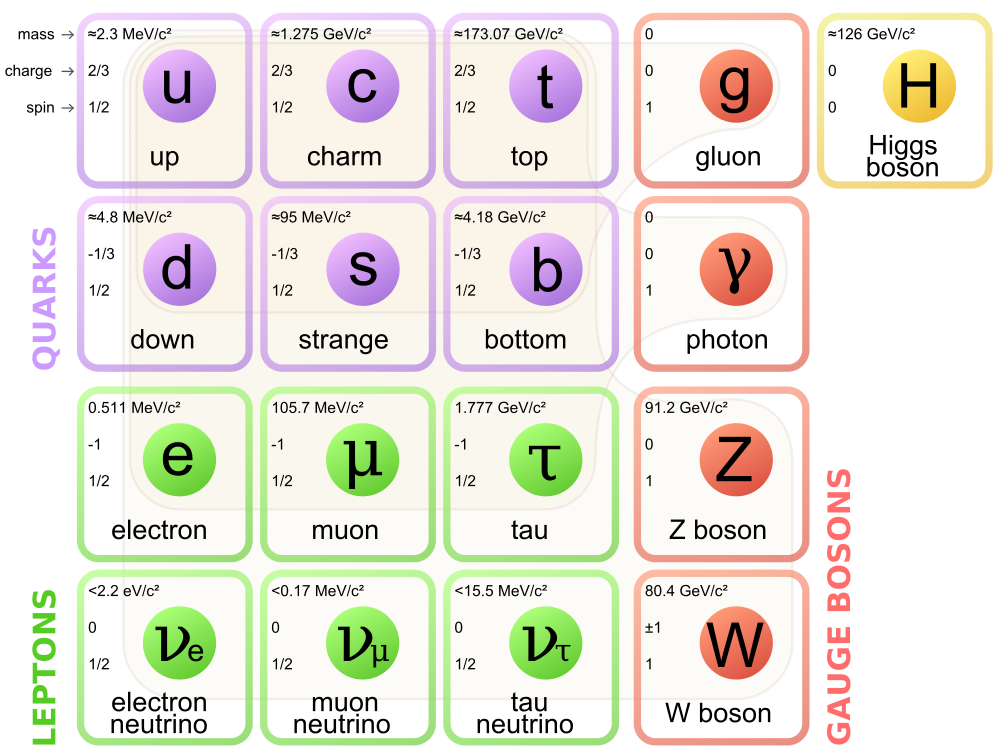
\includegraphics[width=.8\textwidth]{./figures/theory/standardmodel}
	\caption{Standard Model of elementary particle physics\protect\footnotemark.}
	\label{fig:standard_model}
\end{figure}
\footnotetext{{Image source: \url{https://commons.wikimedia.org/wiki/File:Standard_Model_of_Elementary_Particles.svg}, accessed 05/08/2016.}}

\subsection{Heavy Vector Boson Z$^0$}

The particle of interest for this experiment is the Z~boson and its decays are studied.
The Z~boson has a mass of \SI{91.2}{GeV} and a decay width of \SI{2.5}{GeV}.
It was discovered in 1983 in collider experiments at CERN.

\subsubsection{Decays of Z$^0$}

Z~bosons can decay in many different ways.
The final state of their decays can contain quarks, charged leptons and neutrinos, although it must be noted, that the top quark can not be produced since it is way heavier than the Z~boson.
Due to conservation laws the Z~boson may produce only pairs of particles and antiparticles (e.g. electron and positron or neutrino and corresponding antineutrino).
In case of production of a quark-antiquark pair the final state particles will form jets.
Because of confinement in QCD the strong interaction becomes stronger for larger distances between two strongly interacting particles.
If quark and antiquark fly apart a QCD field with high energy is created between them, where additional quark-antiquark pairs can be produced.
This process repeats itself as long as the particles have more energy than needed for formation of colourless hadrons.
As a result a hadronic decay of Z~bosons leads to a high number of final state particles, called jets.
Possible Feynman diagrams for the mentioned processes are shown in figure \ref{fig:feynman}.

\begin{figure}[htb]
	\centering
	\begin{subfigure}{.32\textwidth}
		\centering
		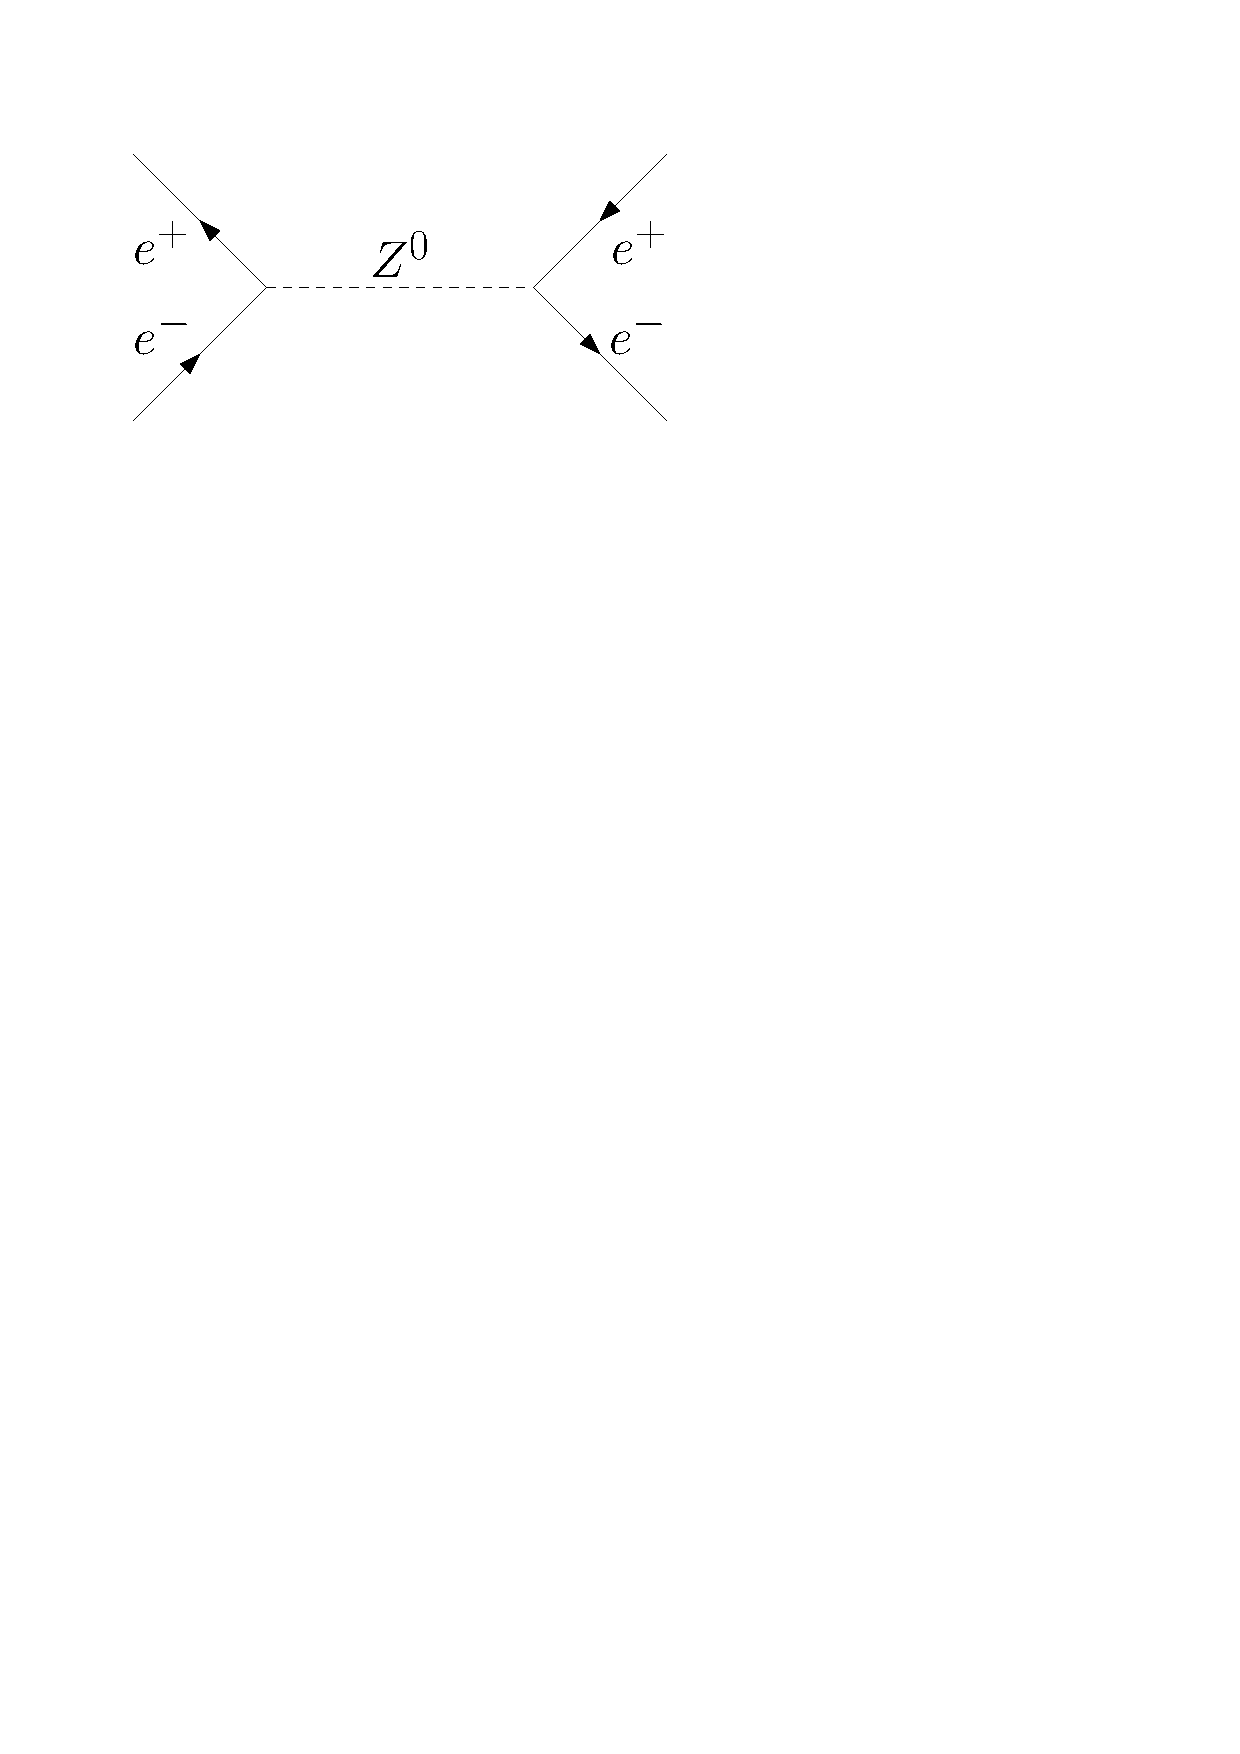
\includegraphics[width=.9\textwidth]{./figures/theory/feynman/ee_s}
		\subcaption{$e^+e^-\rightarrow e^+e^-$ (s-channel)}
	\end{subfigure}
	\begin{subfigure}{.32\textwidth}
		\centering
		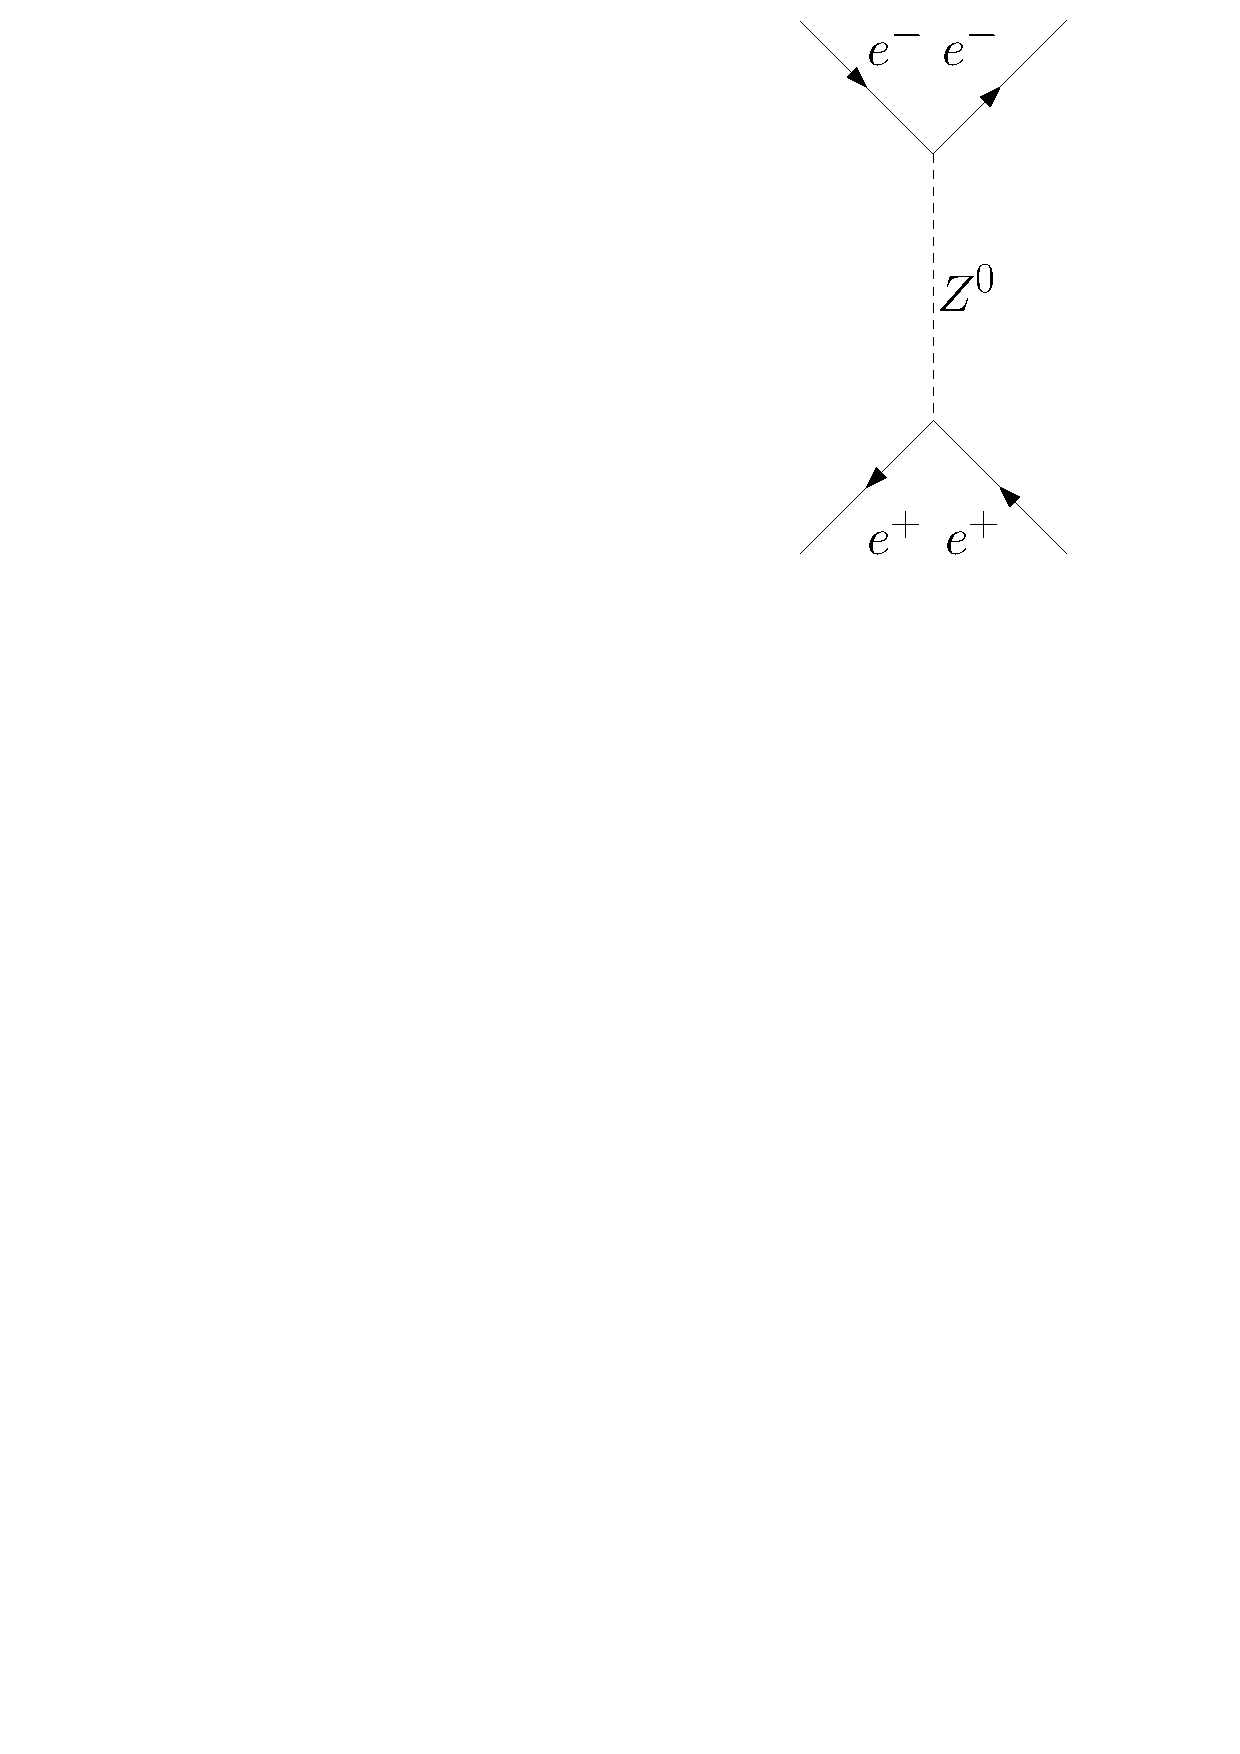
\includegraphics[width=.9\textwidth]{./figures/theory/feynman/ee_t}
		\subcaption{$e^+e^-\rightarrow e^+e^-$ (t-channel)}
	\end{subfigure}
	\begin{subfigure}{.32\textwidth}
		\centering
		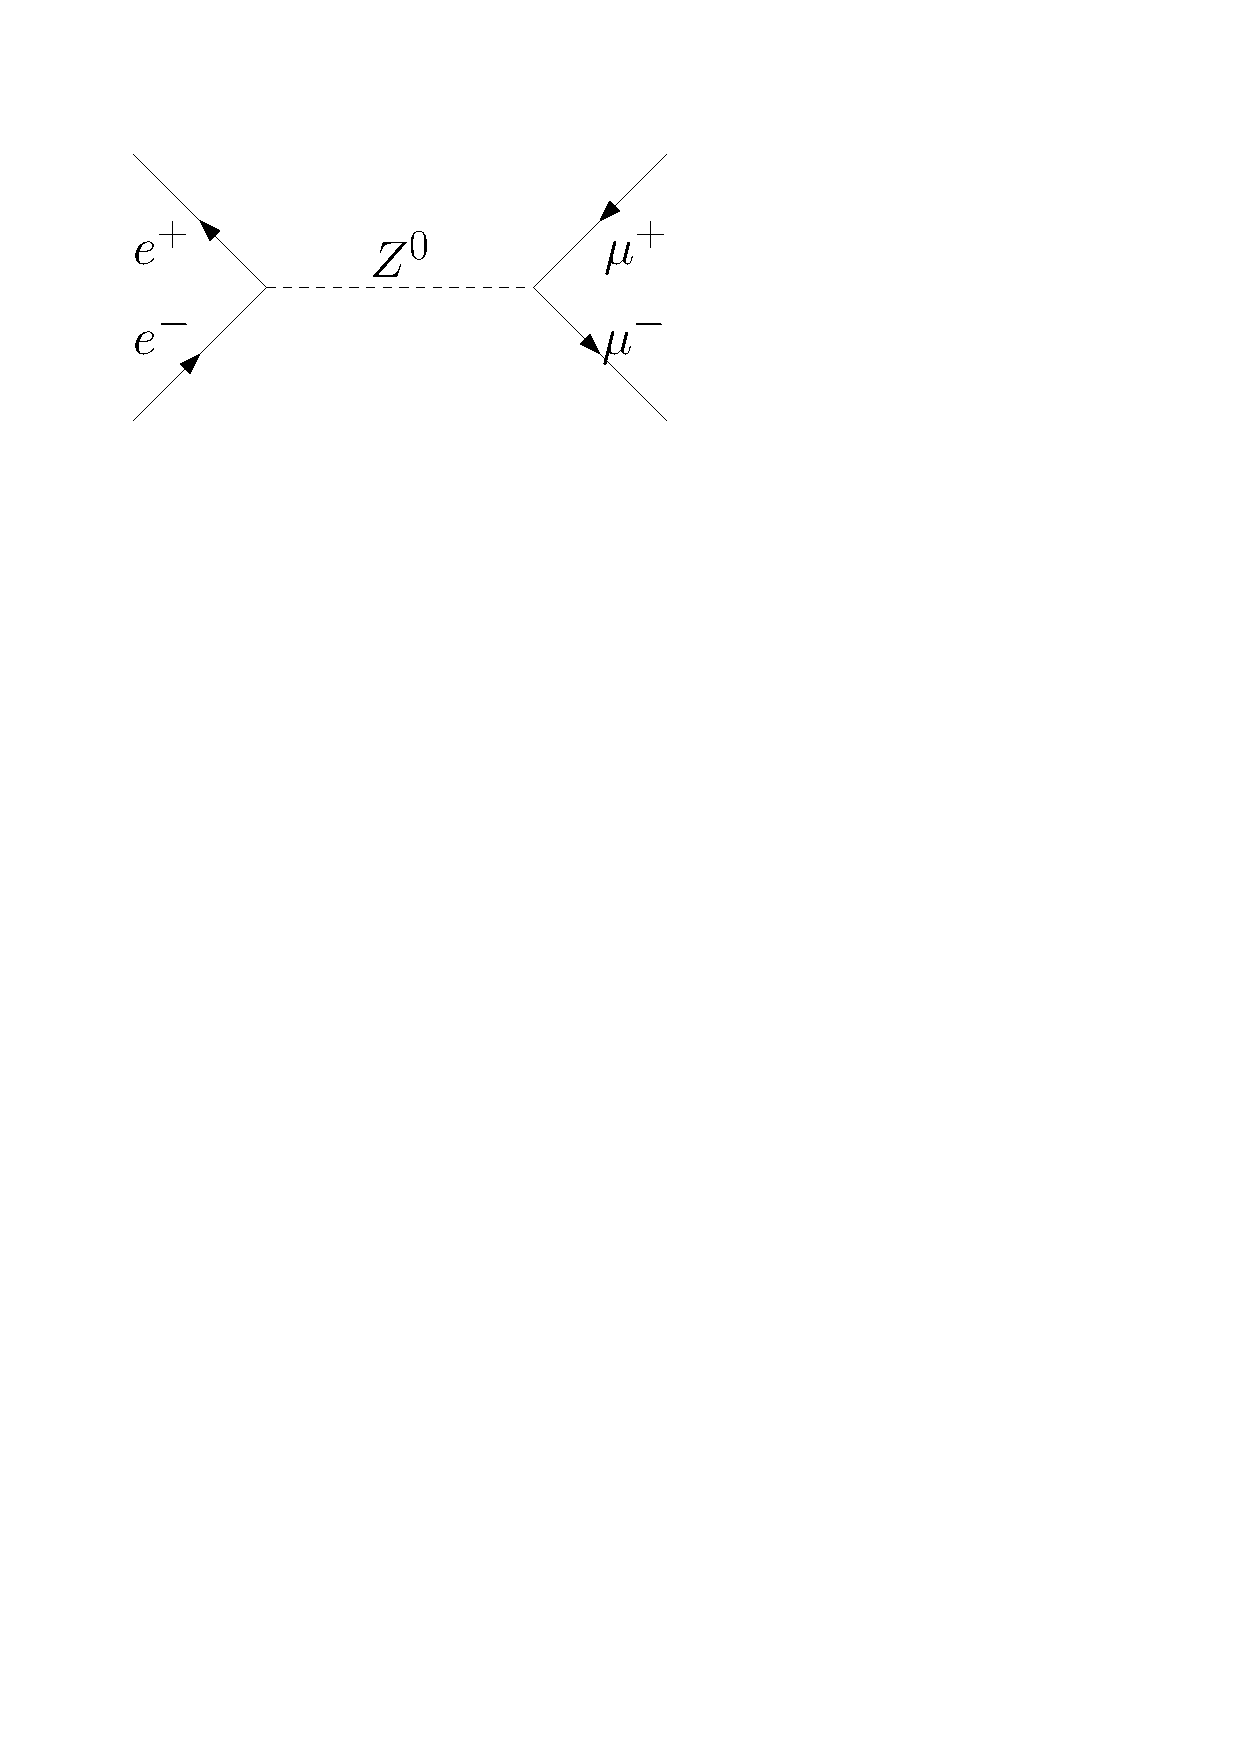
\includegraphics[width=.9\textwidth]{./figures/theory/feynman/mm}
		\subcaption{$e^+e^-\rightarrow \mu^+\mu^-$}
	\end{subfigure}
	\\
	\vspace{2em}
	\begin{subfigure}{.32\textwidth}
		\centering
		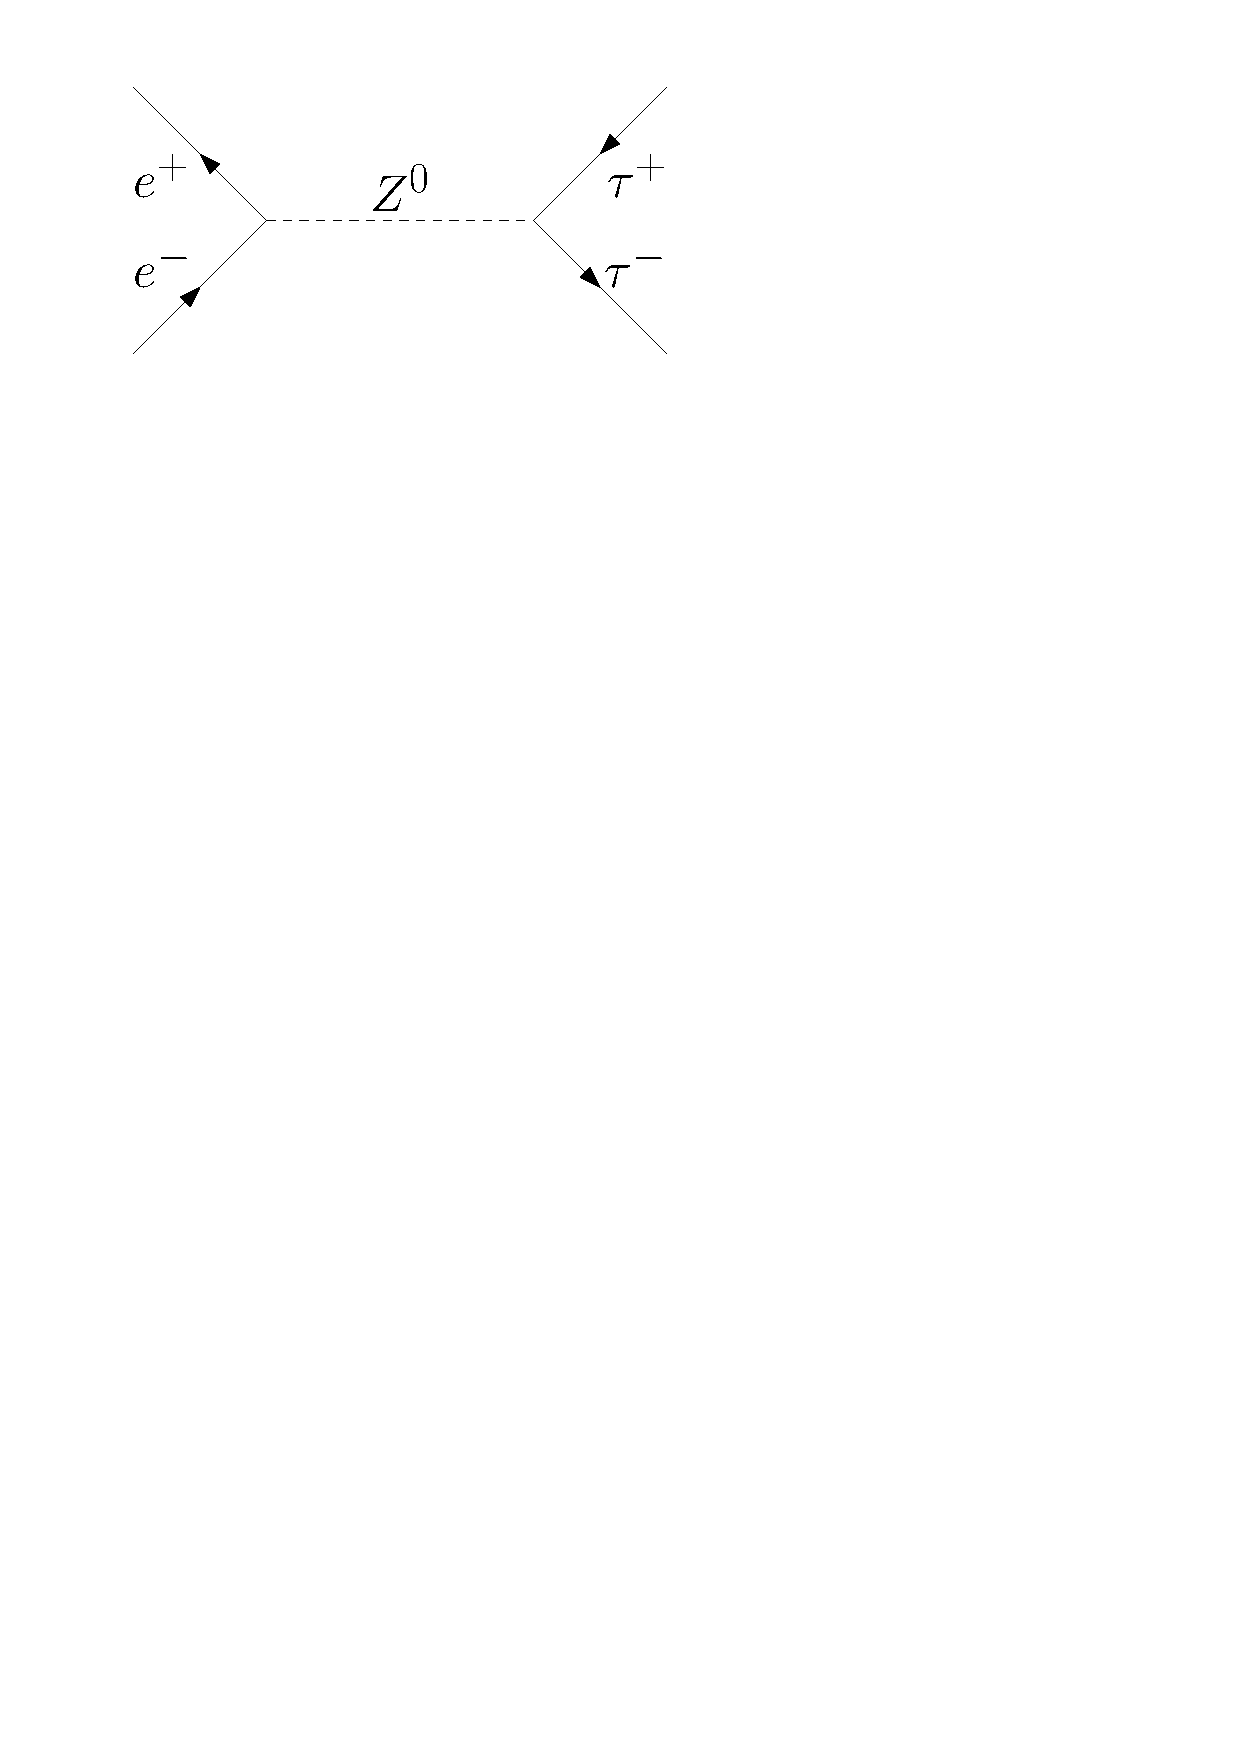
\includegraphics[width=.9\textwidth]{./figures/theory/feynman/tt}
		\subcaption{$e^+e^-\rightarrow \tau^+\tau^-$}
	\end{subfigure}
	\begin{subfigure}{.32\textwidth}
		\centering
		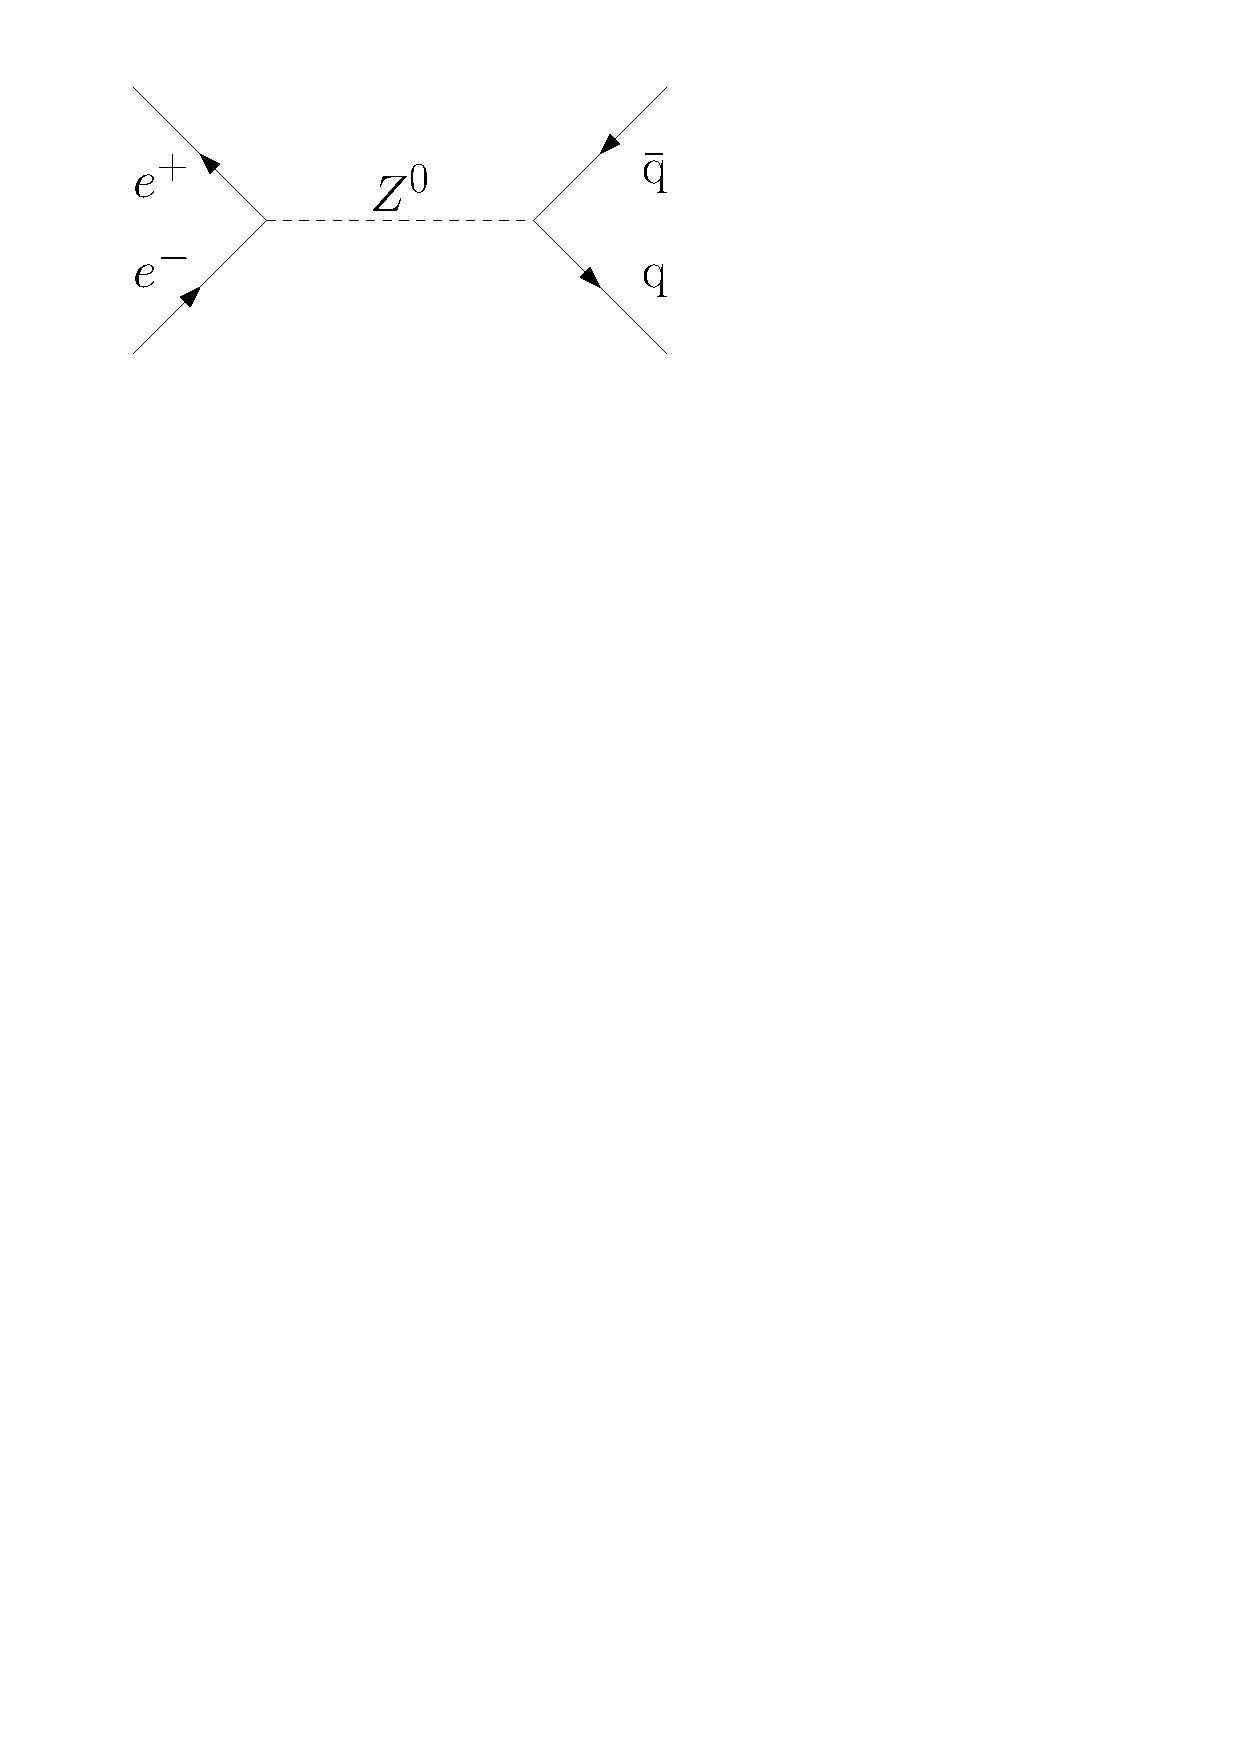
\includegraphics[width=.9\textwidth]{./figures/theory/feynman/qq}
		\subcaption{$e^+e^-\rightarrow \mathrm{q}\mathrm{\bar{q}}$}
	\end{subfigure}
	\begin{subfigure}{.32\textwidth}
		\centering
		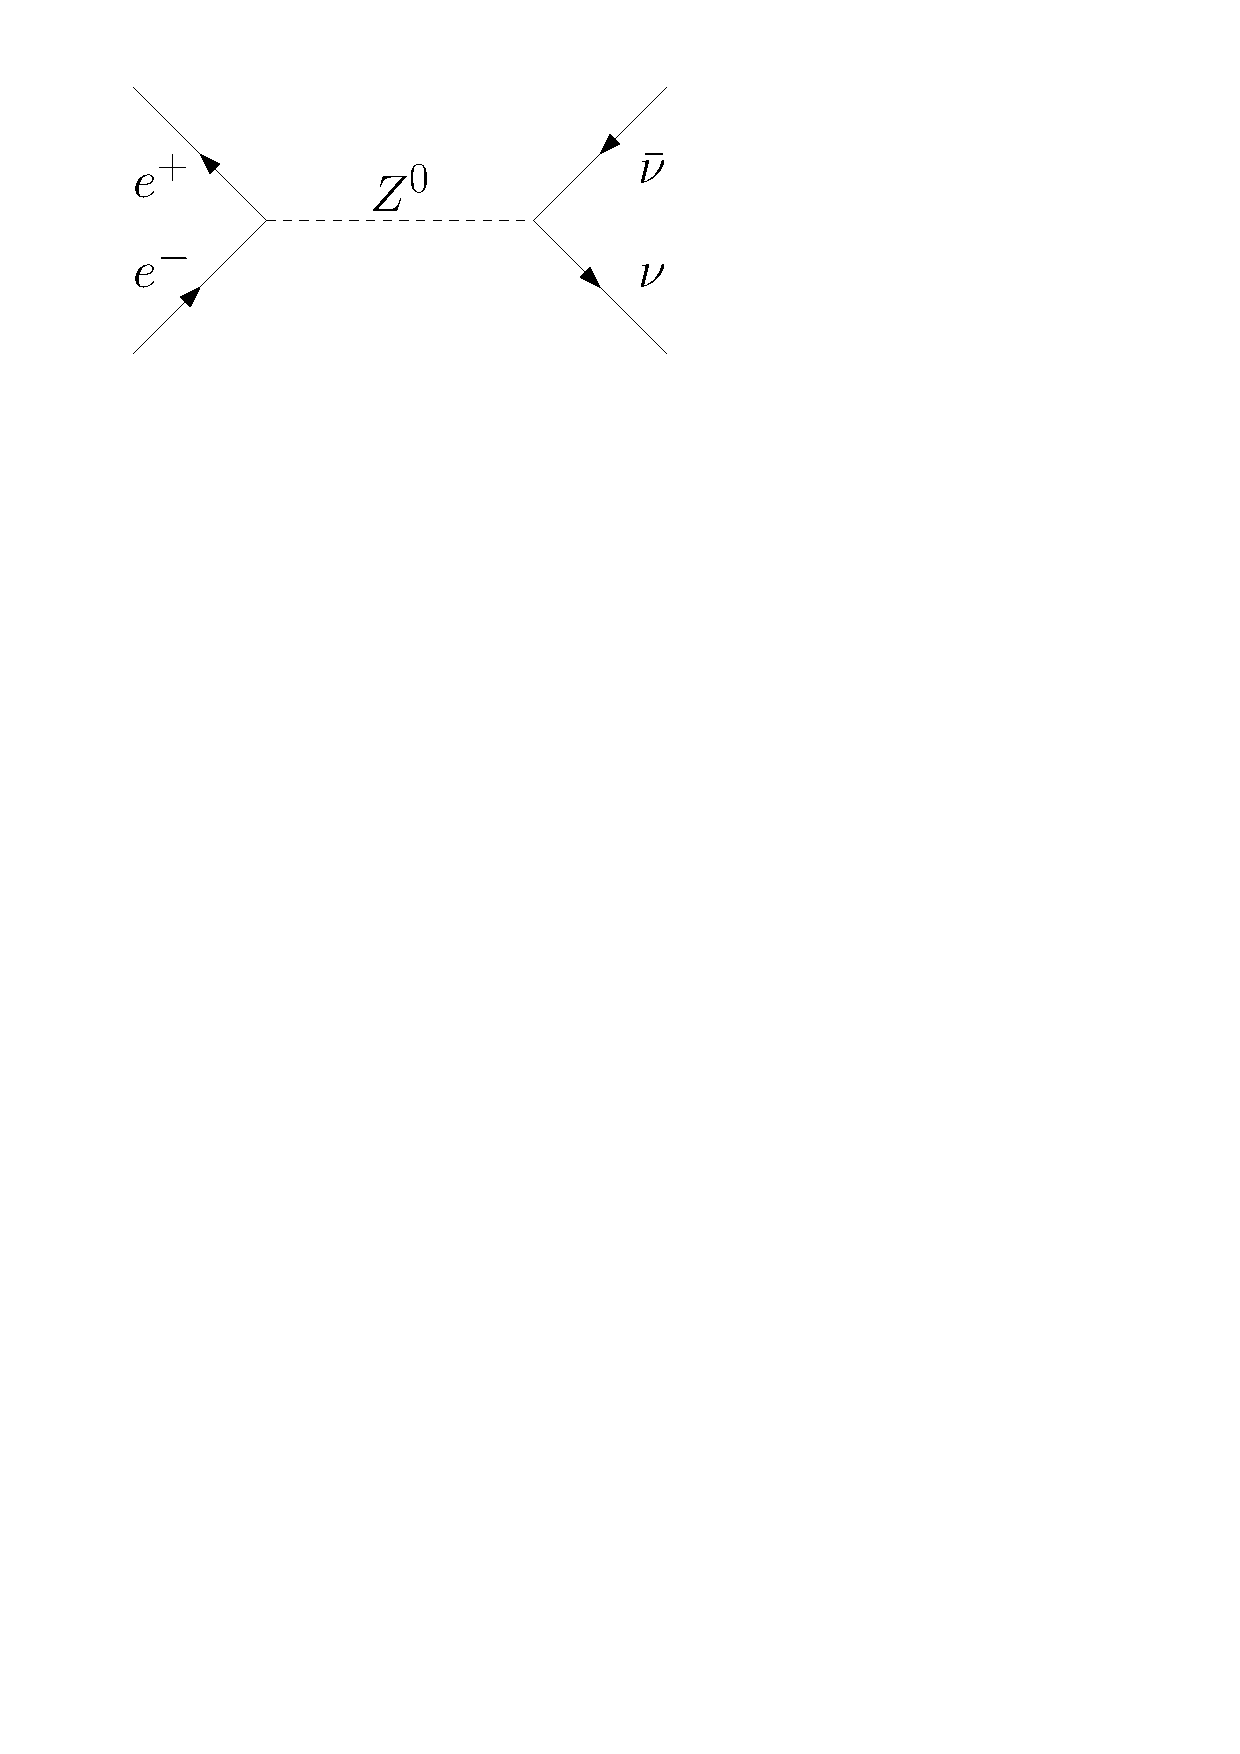
\includegraphics[width=.9\textwidth]{./figures/theory/feynman/nn}
		\subcaption{$e^+e^-\rightarrow \nu\bar{\nu}$}
	\end{subfigure}
	\caption{Feynman diagrams for the different decay channels of the $Z$-boson in lowest order. The initial state is according to the LEP storage ring always assumed to be an electron positron pair. In general, these processes are except for the creation of a neutrino pair also possible with a photon propagator.}
	\label{fig:feynman}
\end{figure}

\subsubsection{Forward-Backward Asymmetry A$_\mathrm{FB}$}

In a $e^+e^- \rightarrow f\bar{f}$ reaction the differential cross section of the produced fermions is different for the forward and backward hemispheres.
Those are defined by the angle $\theta$ between incoming positron and outgoing positively charged particle.
In this lab experiment, the asymmetry A$_\mathrm{FB}$ is measured in $e^+e^- \rightarrow \mu^+\mu^-$ events. 
The asymmetry $A_\mathrm{FB}$is defined by
\begin{align*}
	A_\mathrm{FB}=\frac{\int_{0}^{1}{\deriv{\sigma}{\cos\Theta}}\dinf{\cos\Theta}-\int_{-1}^{0}{\deriv{\sigma}{\cos\Theta}}\dinf{\cos\Theta}}{\int_{0}^{1}{\deriv{\sigma}{\cos\Theta}}\dinf{\cos\Theta}+\int_{-1}^{0}{\deriv{\sigma}{\cos\Theta}}\dinf{\cos\Theta}}
\end{align*}
with the cross-section $\sigma$ and the angle $\Theta$ between incoming positron and outgoing positively charged muon \cite{instructions}.
For a center of mass energy $\sqrt{s}=M_\mathrm{Z^0}$ and by restricting oneself to leptons this can be approximated by \cite{instructions}
\begin{align*}
	A_\mathrm{FB}^{\ell\text{,peak}}\approx 3\left(\frac{v_\ell}{a_\ell}\right)^2\quad\text{.}
\end{align*}
For an explanation of the parameters $v_\ell$ and $a_\ell$, see section \ref{sec:problems}.

\subsection{The OPAL Experiment}

The OPAL~detector shown in \ref{fig:opal} was used from 1989 to 2000 at the LEP storage ring at the CERN facility in Switzerland.
It was designed to detect all kinds of particles produced in collisions of electrons and positrons.
To cover most of the solid angle it had a barrel-like structure and consisted of a cylinder and two endcaps.
For tracking and vertex reconstruction purposes the inner part is formed by a semiconductor strip detector and multiple proportional chambers.
To measure the momentum of charged particles, the whole inner detector is surrounded by a solenoid which creates a magnetic field.
The solenoid is followed by the calorimeters, first the electromagnetic and after that the hadronic one.
As a last layer muon chambers are installed which consist of a tracking detector themselves.
\begin{figure}[h]
	\centering
	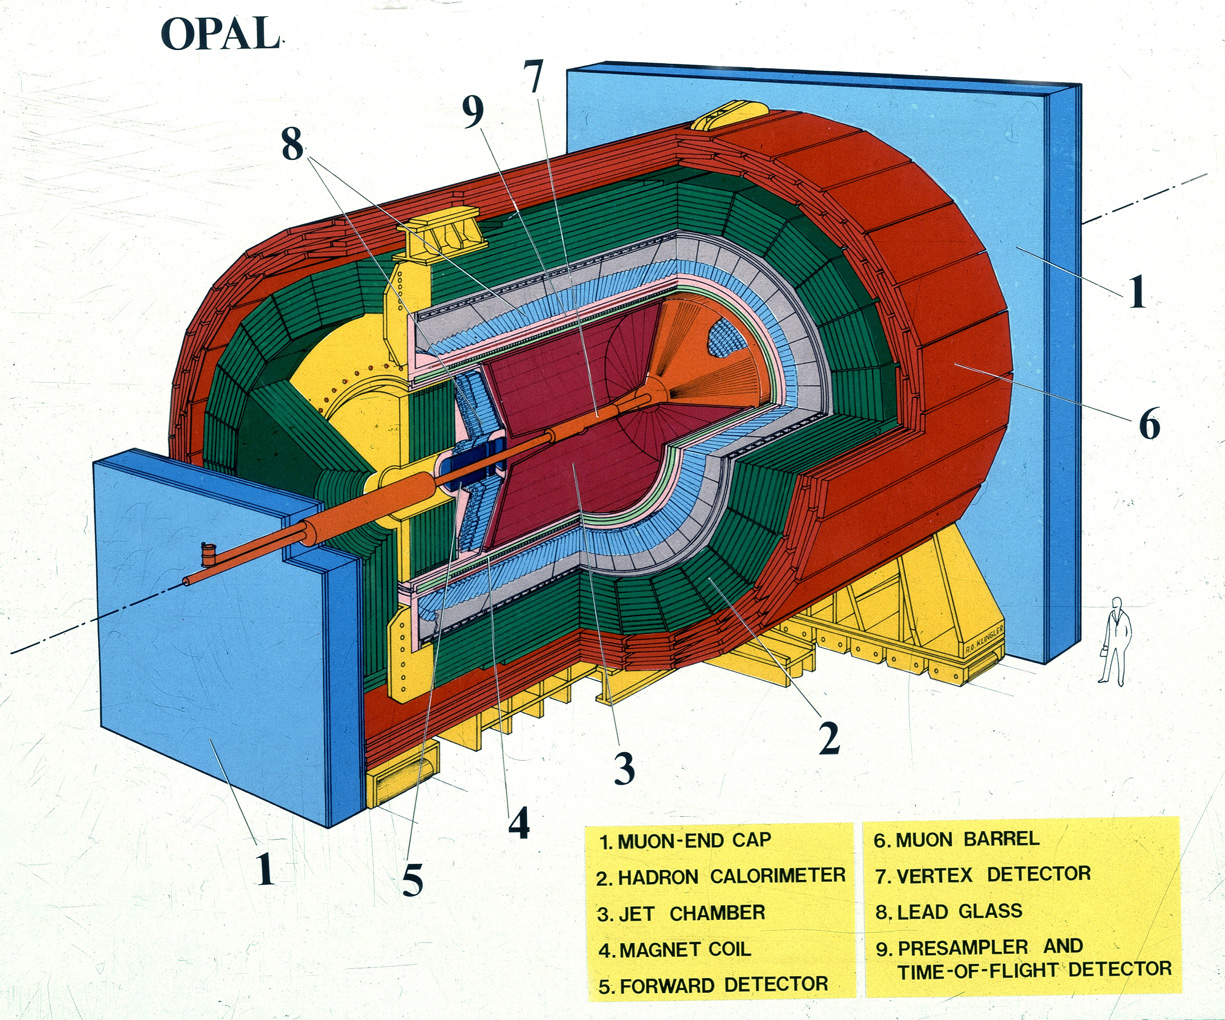
\includegraphics[width=.8\textwidth]{./figures/theory/opal}
	\caption{Cut-away diagram of the OPAL detector with its main components\protect\footnotemark.}
	\label{fig:opal}
\end{figure}
\footnotetext{Image source: CERN-DI-8404652 \url{https://cds.cern.ch/record/39362?ln=en}}

\subsection{Problems}
In the following the questions that should have been solved before performing the experiment are presented.
\label{sec:problems}
\subsubsection{Calculation of Partial Decay Widths}
The theoretical values for the partial decay widths of $Z^0$ decays into charged leptons and hadrons is calculated at first.
This can be done using equation (13) from \cite{instructions}
\begin{align*}
	&\Gamma_f = \frac{N_\mathrm{c}^f \sqrt{2}}{12 \pi} G_\mathrm{F} M_\mathrm{Z}^3 \left( {g_\mathrm{V}^f}^2 + {g_\mathrm{A}^f}^2 \right)
\end{align*}
with the color factor $N_c^f$ which is 1 for leptons and 3 for quarks and the coupling constants
\korr{Tabelle mit weak charges, ladungen und kopplungsfaktoren für die verschiedenen teilchen}
\cite{instructions}
\begin{align*}
	&g_\mathrm{V}^f = I_3^f - 2 Q_f \sin\theta_\mathrm{W}\\
	&g_\mathrm{A}^f = I_3^f \\
	\intertext{for vector and axial-vector coupling that lead to the vector and axial-vector coupling between Z-boson and fermion-antifermion pairs}
	&v_f = \frac{g_\mathrm{V}^f}{2\sin\theta_\mathrm{W}\cos\theta_\mathrm{W}}\\
	&a_f = \frac{g_\mathrm{A}^f}{2\sin\theta_\mathrm{W}\cos\theta_\mathrm{W}}
\end{align*}
The values for the weak charge $Q_f$, the third component of the weak isospin $I_3^f$ and the Weinberg angle $\theta_\mathrm{W}$ are given in table \korr{REF}\\
Partial widths
\begin{align*}
	&\Gamma_\ell = \SI{83.4}{MeV} \\
	&\Gamma_\nu = \SI{165.9}{MeV} \\
	&\Gamma_\mathrm{u} = \SI{285.3}{MeV} \\
	&\Gamma_\mathrm{d} = \SI{367.8}{MeV}
\end{align*}
\korr{u und d jeweils für alle up- bzw down-type Quarks}
\begin{align*}
\Gamma_\mathrm{hadrons} &= 2\Gamma_\mathrm{u} + 3\Gamma_\mathrm{d} \\
&= \SI{1.67}{GeV}
\end{align*}
\begin{align*}
	\Gamma_\mathrm{ch.~leptons} = 3\Gamma_\ell = \SI{250}{MeV}
\end{align*}
\begin{align*}
	\Gamma_\mathrm{neutrinos} = 3\Gamma_\nu =\SI{498}{MeV}
\end{align*}

total decay width
\begin{align*}
	\Gamma_\mathrm{Z} &= \Gamma_\mathrm{hadrons} + 3 \Gamma_\ell + 3\Gamma_\nu \\
	&= \SI{2.42}{GeV}
\end{align*}

\subsubsection{Partial Cross Sections}
\cite{instructions}
\begin{align*}
	\sigma_f^\mathrm{peak} = \frac{12 \pi}{M_\mathrm{Z}^2} \frac{\Gamma_\mathrm{e}}{\Gamma_\mathrm{Z}} \frac{\Gamma_f}{\Gamma_\mathrm{Z}}
\end{align*}

\begin{align*}
	&\sigma_\ell^\mathrm{peak} = \SI{2.09}{nb}\\
	&\sigma_\nu^\mathrm{peak} = \SI{4.16}{nb}\\
	&\sigma_\mathrm{u}^\mathrm{peak} = \SI{7.16}{nb} \\
	&\sigma_\mathrm{d}^\mathrm{peak} = \SI{9.23}{nb} 
\end{align*}

\subsubsection{Decay into additional pair???}
\korr{Formel?}
\begin{align*}
	&\mathrm{ch.~lepton:} ~ 3.4\% \\
	&\mathrm{up~type:} ~ 11.8 \% \\
	&\mathrm{down~type:} ~ 15.2 \% \\
	&\mathrm{neutrino:} ~ 6.9 \%
\end{align*}

\subsubsection{Angular distribution}
\korr{noch summe (wie sind die einzelnen channels normiert?) und verteilung für muonen}
\begin{figure}
	\centering
	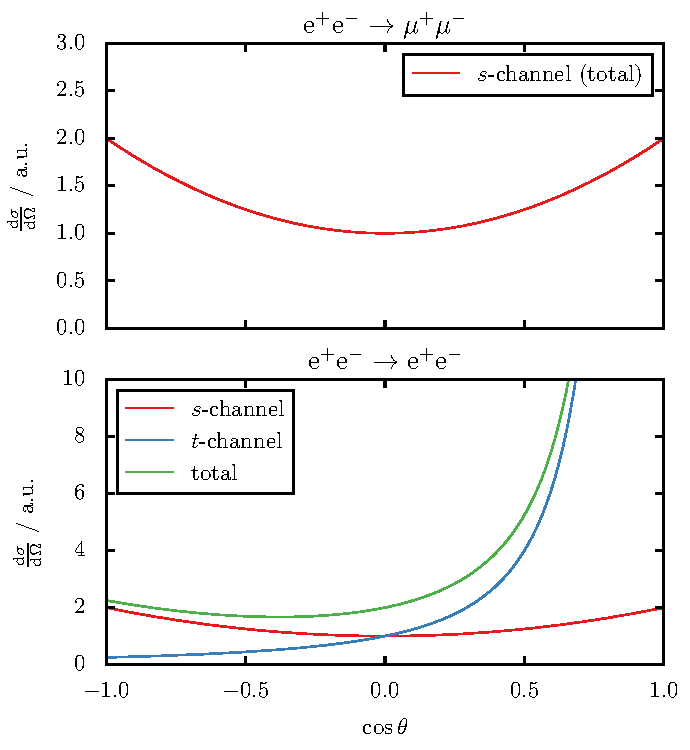
\includegraphics{./figures/s_t_channel.pdf}
	\caption{Bla \korr{proportionalitäten erwähnen. Und erwähnen dass s und t channel mit der gleichen proportionalitätskonstante in die summe eingehen was in der realität nicht unbedingt der fall sein muss. erklären wie man jetzt den s-channel filtert.}}
\end{figure}

\subsubsection{Forward-backward Asymmetry}

\begin{table}[h]
	\centering
	\begin{tabular}{cl|ccc}
	& 			& \multicolumn{3}{c}{center of mass energy $\sqrt{s}$} 		\\
	&			& \SI{89.225}{GeV} 	& \SI{91.225}{GeV} 	& \SI{93.225}{GeV} 	\\\hline
	\multirow{3}{*}{\rotatebox{90}{$\sin^2\theta_\mathrm{W}$}}
	& \num{0.21} 	& \num{-0.094} 		& \num{0.076}		& \num{0.232}		\\
	& \num{0.23} 	& \num{-0.164}		& \num{0.023}		& \num{0.196}		\\
	& \num{0.25}	& \num{-0.195}		& \num{0.004}		& \num{0.191} 		\\	
	\end{tabular}
	\caption{Values for $A_\mathrm{FB}$ calculated with the exact formula (20) given in \cite{instructions} for different center of mass energies and Weinberg angles.}
\end{table}





\section{Part I: Analysis of Event Displays}

On the first day the software \texttt{GROPE} was used to study event displays and detector responses of the OPAL detector.

\subsection{Classification of Events by Detector Response}

To learn how to distinguish the different decay channels of the Z boson Monte-Carlo simulated test samples with events with only one decay mode have been investigated.
In the following part the measured properties of the observed events and exemplary pictures of the detector response are presented.
The variables given for every event are presented in table \ref{tab:desc_variables_tag1}
\begin{table}[H]
	\centering
	\begin{tabularx}{0.9\textwidth}{lX}
		\toprule
		\textbf{Variable} & \textbf{Description} \\
		\midrule		
		Ctrk(N) 	& Number of charged particle tracks in the tracking detector \\
		Ctrk(SumP) 	& Total momentum of all charged particle tracks in the tracking detector \\
		Ecal(SumE)	& Total energy deposited in the electromagnetic calorimeter \\
		Hcal(SumE)	& Total energy deposited in the hadronic calorimeter \\
		\bottomrule
	\end{tabularx}
	\caption{Description of the variables in the $\mathrm{Z}^0$ decay datasets. Momenta and energies are always given in units of GeV.}
	\label{tab:desc_variables_tag1}
\end{table}
Deviations from ideal signals can always occur and have been noted in the tables.
Those can originate either as additional signals from background radiation, e.g. cosmic muons or as deviations from the expected theoretical detector response, e.g. bremsstrahlung photons being emitted from electrons in the initial and final state can cause kinks in the tracks.

\clearpage
\subsubsection{Z$^0\rightarrow e^+e^-$}

A decay into electrons can easily be identified by the energy deposited in the electromagnetic calorimeters.
The final state particles are flying approximately in opposite direction and are ideally completely stopped in the electromagnetic calorimeter.
A track for every particle can be observed in the tracking chamber.
Additional hits in the electromagnetic calorimeters probably occur due to bremsstrahlung photons which leave no track in the inner detector.
\begin{sidewaystable}
	\centering
	\begin{tabular}{ccccccl}
	\toprule
	Run & Event & Ctrk(SumP) & Ctrk(N) & Ecal (SumE) & Hcal (SumE) & Comments \\
	\midrule
	2566 & 163733 & 50.9       & 2       & 82.6       & 0.0        &  not exactly back to back electrons, initial or final state radiation\\
	2566 & 165523 & 91.9       & 2       & 90.0       & 0.0        &  \\
	2566 & 165548 & 82.5       & 3       & 92.3       & 0.0        &  \\
	2566 & 165576 & 80.9       & 2       & 86.8       & 0.0        &  \\
	2566 & 166436 & 38.1       & 2       & 89.5       & 0.0        &  \korr{Bremsstrahlung?}\\
	2566 & 167987 & 83.8       & 2       & 87.5       & 0.0        &  \\
	2566 & 168389 & 87.4       & 2       & 93.2       & 0.0        &  \\
	2566 & 170045 & 69.3       & 2       & 90.7       & 0.0        &  \\
	2566 & 170379 & 86.1       & 2       & 89.4       & 0.5        &  \\
	2566 & 197594 & 90.3       & 2       & 90.6       & 0.0        &  \\
	2566 & 197889 & 92.1       & 2       & 88.5       & 0.5        &  \\
	2570 & 28178  & 81.7       & 3       & 91.6       & 0.0        &  third track starting at interaction point observable\\
	2570 & 28499  & 89.6       & 2       & 92.5       & 0.0        &  \\
	2570 & 28743  & 61.1       & 2       & 89.2       & 0.0        &  \korr{Bremsstrahlung?}\\
	2570 & 28777  & 88.4       & 3       & 89.1       & 0.0        &  third track present that follows a helix, probably $\delta$ electron\\
	2570 & 88224  & 90.9       & 2       & 90.5       & 0.3        &  \\
	2570 & 90060  & 64.6       & 2       & 88.8       & 0.0        &  \korr{Bremsstrahlung?}\\
	2570 & 91274  & 95.6       & 2       & 96.2       & 0.0        &  \\
	2571 & 418921 & 93.0       & 2       & 90.8       & 0.0        &  \\
	2571 & 420590 & 94.1       & 2       & 89.2       & 0.0        &  \\
	\bottomrule
\end{tabular}
	\caption{Collected data from the electron dataset. All values for energies and momenta in \si{GeV}.}
\end{sidewaystable}
\begin{figure}[h]
	\centering
	\begin{subfigure}{\textwidth}
		\centering
		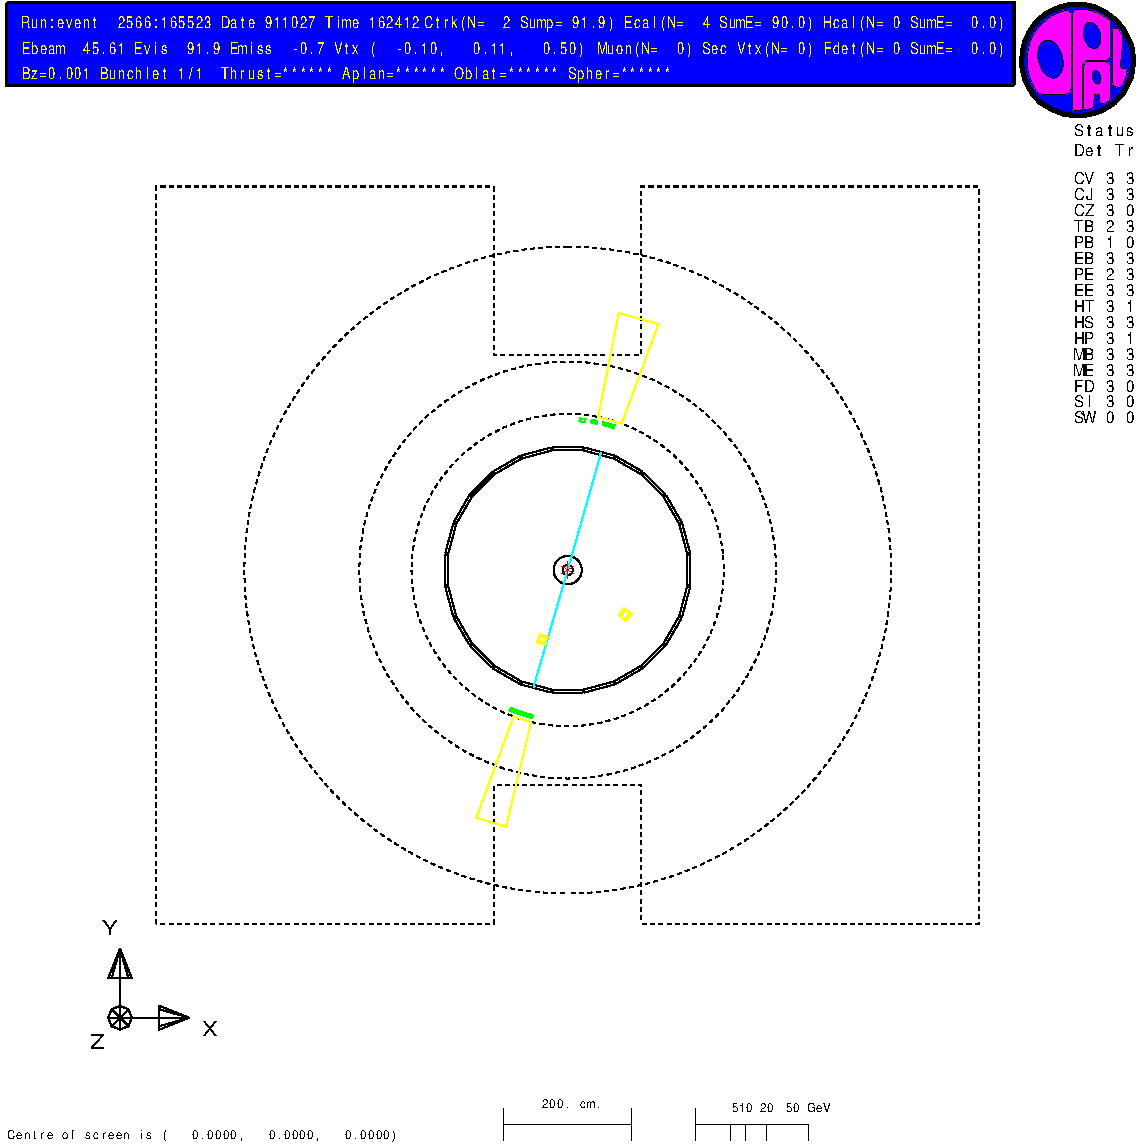
\includegraphics[width=.75\textwidth]{./data/tag1/ee_pics/cropped/ee_02}
		\subcaption{Front view}
	\end{subfigure}
	\begin{subfigure}{\textwidth}
		\centering
		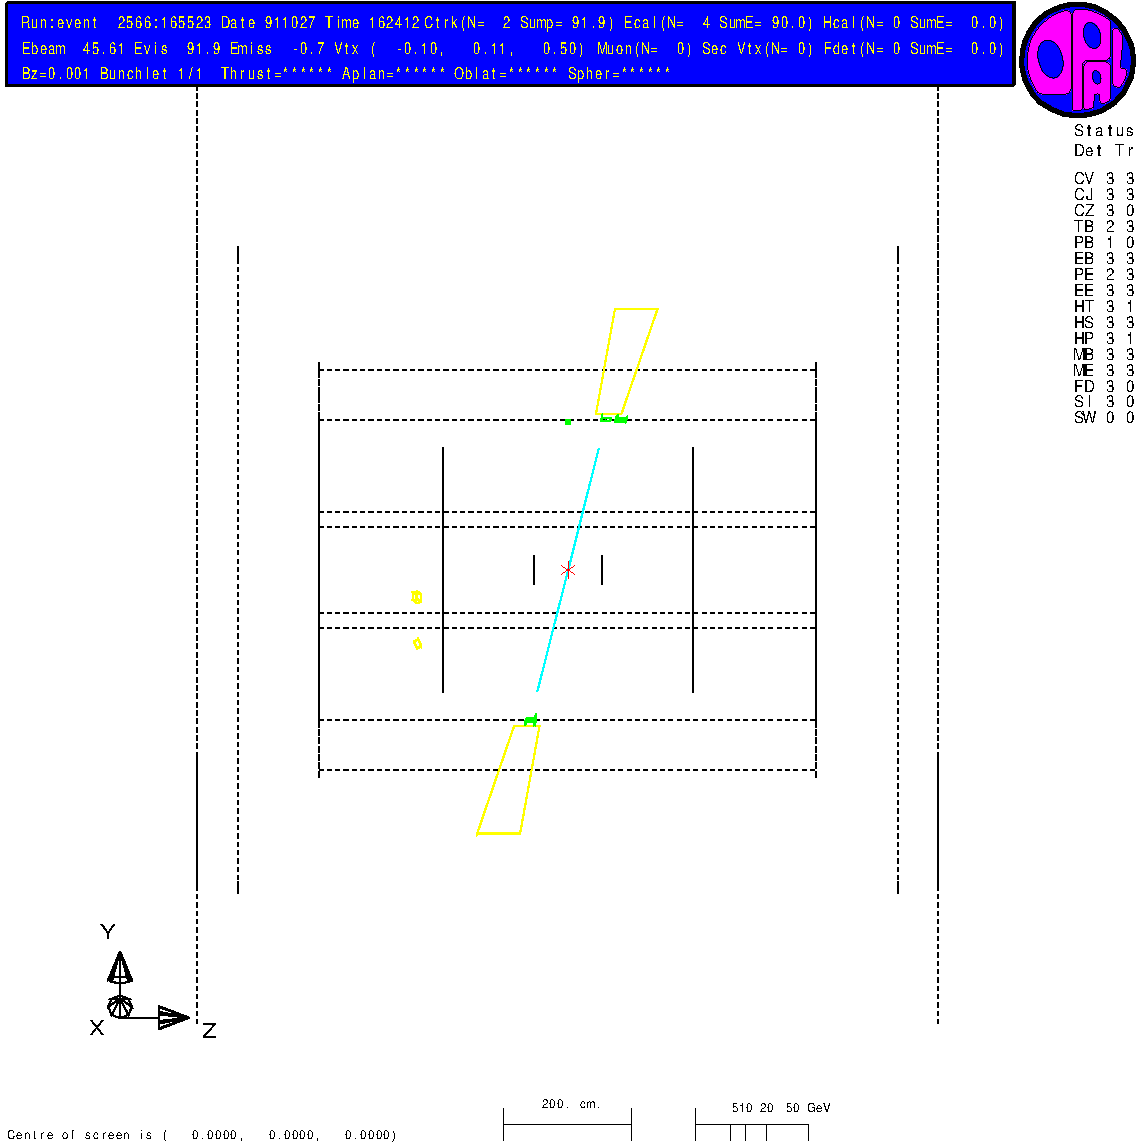
\includegraphics[width=.75\textwidth]{./data/tag1/ee_pics/cropped/ee_02_side}
		\subcaption{Side view}
	\end{subfigure}
	\caption{Exemplary picture of a $Z^0\rightarrow e^+e^-$ event. Electron and positron are emitted back to back, leave a track in the inner detector (light blue) and are stopped in the electromagnetic calorimeter (yellow).}
\end{figure}
\clearpage
\subsubsection{Z$^0\rightarrow \mu^+\mu^-$}

Muons are detected in the muon chambers which form the outermost part of the detector.
Since all other particles (except the non-detectable neutrinos) are stopped before reaching the muon chamber a detected particle there can be identified as a muon. 
In general, muons are also created in a back to back configuration and leave a track in the tracking detector.
\begin{sidewaystable}
	\centering
	\begin{tabular}{ccccccl}
	\toprule
	Run & Event & Ctrk(SumP) & Ctrk(N) & Ecal (SumE) & Hcal (SumE) & Comments \\
	\midrule
	2568 & 80617  & 90.1  & 2 & 1.6 & 7.0  &  \\ \midrule
	2568 & 84297  & 93.0  & 2 & 1.6 & 8.7  &  \\
	2568 & 85398  & 96.8  & 2 & 2.0 & 0.0  &  \\
	2568 & 87693  & 89.1  & 2 & 2.3 & 8.5  &  \\
	2568 & 89929  & 90.5  & 2 & 1.5 & 7.2  &  \\
	2568 & 91048  & 91.8  & 2 & 1.8 & 4.3  &  \\
	2568 & 92681  & 86.3  & 2 & 3.7 & 3.3  &  three hits, one could be cosmic, not coming from IP\\
	2568 & 93199  & 99.2  & 2 & 1.3 & 2.9  &  \\
	2568 & 95202  & 88.2  & 2 & 1.6 & 3.0  &  \\
	2568 & 99962  & 90.9  & 2 & 1.3 & 6.7  &  \\
	2568 & 100566 & 95.6  & 2 & 2.5 & 6.1  &  \\
	2568 & 100721 & 75.3  & 2 & 3.1 & 6.8  &  bent track due to initial state radiation \\
	2568 & 102167 & 85.2  & 2 & 5.8 & 4.4  &  \\
	2568 & 105720 & 98.6  & 2 & 3.6 & 5.7  &  \\
	2568 & 106346 & 86.8  & 2 & 1.9 & 7.9  &  \\
	2568 & 107030 & 98.0  & 2 & 1.9 & 2.0  &  \\
	2568 & 107772 & 108.3 & 2 & 2.0 & 8.5  &  one of the muons created two hits, three muon hits in total\\
	2568 & 108553 & 92.4  & 2 & 3.6 & 6.7  &  \\
	2568 & 110610 & 92.0  & 2 & 1.9 & 22.6 & \korr{Warum soviel Hcal? Kann man das erklären?} \\
	2570 & 29023  & 92.6  & 2 & 3.6 & 5.7  &  \\
	\bottomrule
\end{tabular}
	\caption{Collected data from the muon dataset. All values for energies and momenta in \si{GeV}.}
\end{sidewaystable}
\begin{figure}[h]
	\centering
	\begin{subfigure}{\textwidth}
		\centering
		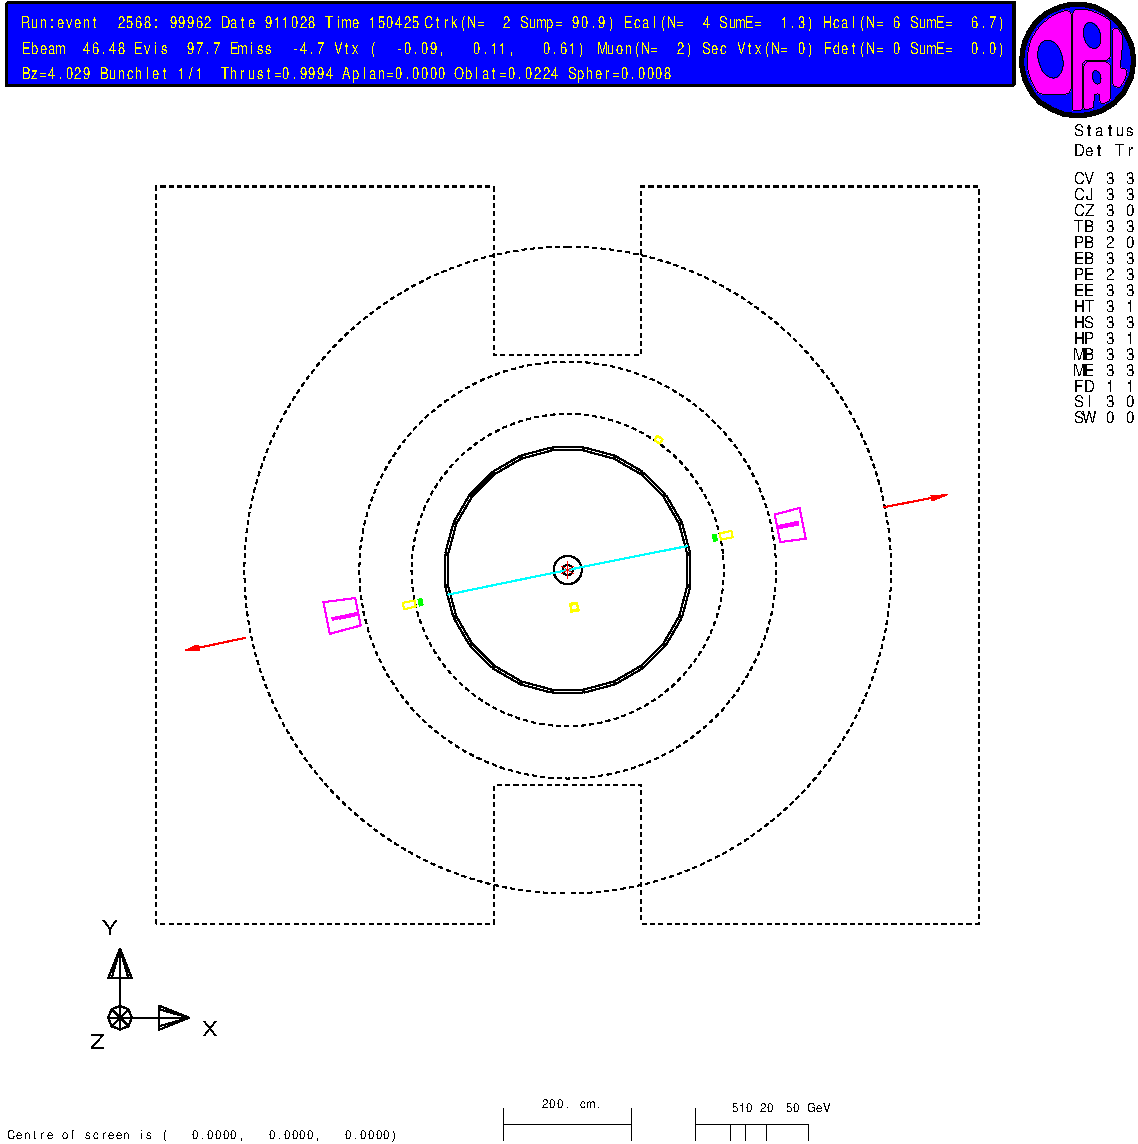
\includegraphics[width=.75\textwidth]{./data/tag1/mm_pics/cropped/mm_02}
		\subcaption{Front view}
	\end{subfigure}
	\begin{subfigure}{\textwidth}
		\centering
		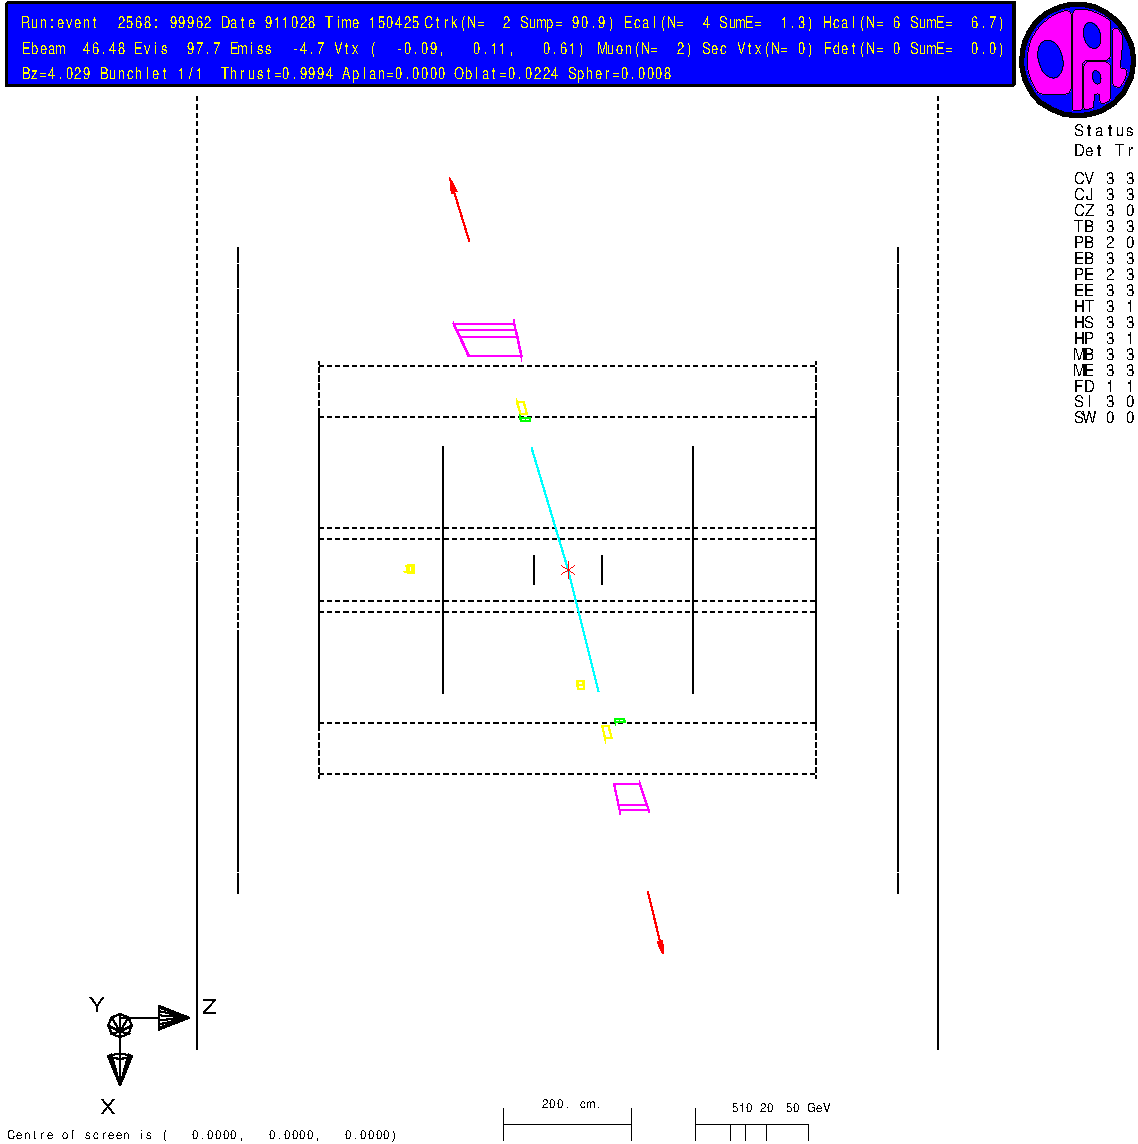
\includegraphics[width=.75\textwidth]{./data/tag1/mm_pics/cropped/mm_02_side}
		\subcaption{Side view}
	\end{subfigure}
	\caption{Exemplary picture of a $Z^0\rightarrow \mu^+\mu^-$ event. The muons are emitted back to back, leave a track in the inner detector (light blue) and small entries in the electromagnetic calorimeter (yellow) and the hadronic calorimeter (purple). They are identified as muons in the muon detector (red arrow).}
\end{figure}
\clearpage
\subsubsection{Z$^0\rightarrow \tau^+\tau^-$}

Because of the short lifetime of the $\tau$ lepton it can not be detected directly but by its decay products.
Because it can decay in both leptons and hadrons there are two possible types of detector responses.
In a leptonic $\tau$ decay an electron or muon and two neutrinos are created and seen as charged tracks in the inner detector.
They cause signals either in the electromagnetic calorimeter or in the muon chambers while the neutrinos are not detected.
Since neutrinos carry momentum this leads to a smaller value for the measured final state compared to the initial state momentum.

In a hadronic $\tau$ decay a neutrino and hadrons are produced.
All hadrons create a shower in the hadronic calorimeter but depending on their charge a track can not always be observed.
\begin{sidewaystable}
	\centering
	\resizebox{\textwidth}{!}{
		\begin{tabular}{ccccccll}
	\toprule
	Run & Event & Ctrk(SumP) & Ctrk(N) & Ecal (SumE) & Hcal (SumE) & Decay & Comments \\
	\midrule
	2566 & 170371 & 74.0 & 5 & 51.1 & 10.2 & 3 $\pi^\pm$, 1 $\pi^\pm$ & 3 and 1 prong \\
	2566 & 170508 & 46.5 & 2 & 17.3 & 8.2  & 1 $\pi^\pm$, 1 $\mu^\pm$ & 1 and 1 prong \\
	2566 & 179750 & 30.8 & 2 & 1.6  & 6.3  & 2 $\mu^\pm$ & 1 and 1 prong  \\
	2566 & 184010 & 29.5 & 2 & 10.2 & 4.1  & 1 $\mu^\pm$, 1 $e^\pm$ & 1 and 1 prong  \\
	2566 & 184435 & 33.1 & 2 & 1.5  & 10.6 & 2 $\mu^\pm$ & 1 and 1 prong  \\
	2566 & 189056 & 24.4 & 2 & 12.4 & 11.7 & 1 $e\pm$, 1 $\pi^\pm$ & 1 and 1 prong \\
	2566 & 208314 & 36.0 & 4 & 16.1 & 5.7  & 1 $\mu^\pm$, 3 $\pi^\pm$ & 1 and 3 prong  \\
	2566 & 212745 & 41.3 & 2 & 11.1 & 20.0 & 1 $e^\pm$, 1 $\mu^\pm$ & 1 and 1 prong \\
	2570 & 29664  & 49.7 & 2 & 5.2  & 20.3 & 2 $\mu^\pm$ & 1 and 1 prong, additional muon, probably cosmic background \\
	2570 & 30348  & 33.4 & 2 & 23.6 & 6.9  & 1 $e^\pm$, 1 $\mu^\pm$ & 1 and 1 prong  \\
	2570 & 34612  & 14.1 & 2 & 3.3  & 6.3  & 1 $\mu^\pm$, 1 $\pi^\pm$ & 1 and 1 prong  \\
	2570 & 39992  & 19.7 & 2 & 15.9 & 3.8  & 1 $e\pm$, 1 $\pi^\pm$ & 1 and 1 prong \\
	2570 & 42200  & 26.8 & 2 & 16.5 & 3.4  & 1 $\mu^\pm$, 1 $e^\pm$ & 1 and 1 prong \\
	2570 & 45609  & 23.4 & 5 & 27.0 & 17.1 & 1 $\mu^\pm$, 1 $\pi^\pm$ & 1 and 1 prong, one additional conversion photon \\
	2570 & 47033  & 23.8 & 2 & 29.4 & 3.6  & 2 $e^\pm$ & 1 and 1 prong \\
	2572 & 98915  & 39.0 & 2 & 18.9 & 4.4  & 1 $\mu^\pm$, 1 $e^\pm$ & 1 and 1 prong \\
	2572 & 102412 & 24.1 & 2 & 46.5 & 7.3  & 1 $e\pm$, 1 $\pi^\pm$ & 1 and 1 prong \\
	2572 & 102586 & 38.5 & 5 & 28.5 & 0.0  & 1 $e^\pm$, 3 $\pi^\pm$ & 1 and 3 prong, possible additional cosmic radiation \\
	2572 & 108411 & 35.3 & 2 & 51.8 & 2.3  & 2 $\pi^\pm$ & 1 and 1 prong, additional $\pi^0$ decaying to photon \\
	2572 & 109621 & 17.8 & 2 & 2.5  & 5.0  & 2 $\mu^\pm$ & 1 and 1 prong, in total four muon hits due to cosmic background \\
	\bottomrule
\end{tabular}
	}
	\caption{Collected data from the tau dataset. All values for energies and momenta in \si{GeV}. To identify the decay, only the charged particles are given. There are always neutrinos present which can not be detected and often times it is possible to have $\pi^0$ mesons that interact electromagnetically.}
\end{sidewaystable}
\begin{figure}[h]
	\centering
	\begin{subfigure}{\textwidth}
		\centering
		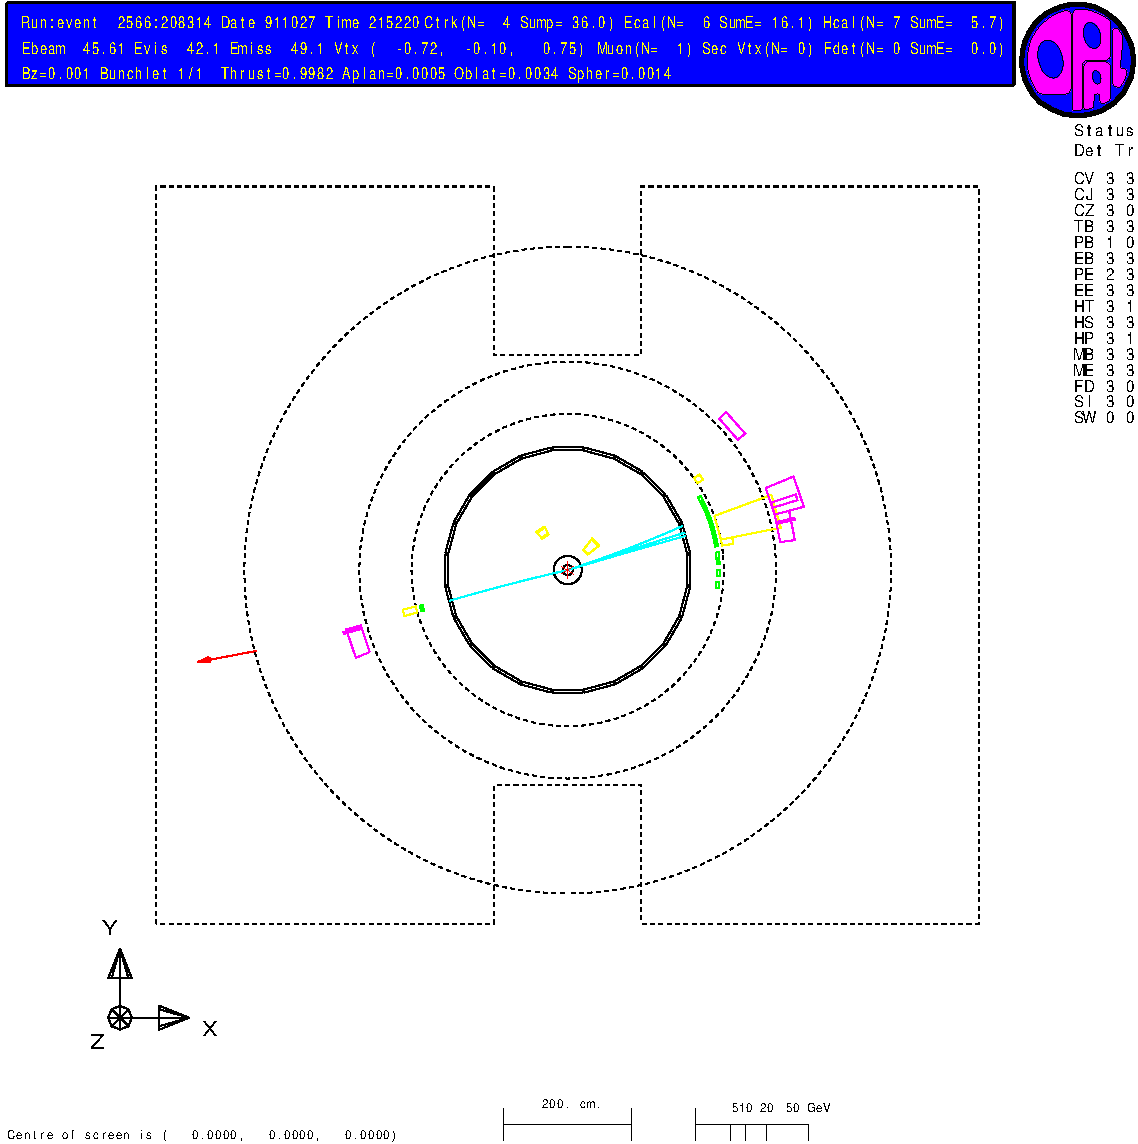
\includegraphics[width=.75\textwidth]{./data/tag1/tt_pics/cropped/tt_05}
		\subcaption{Front view}
	\end{subfigure}
	\begin{subfigure}{\textwidth}
		\centering
		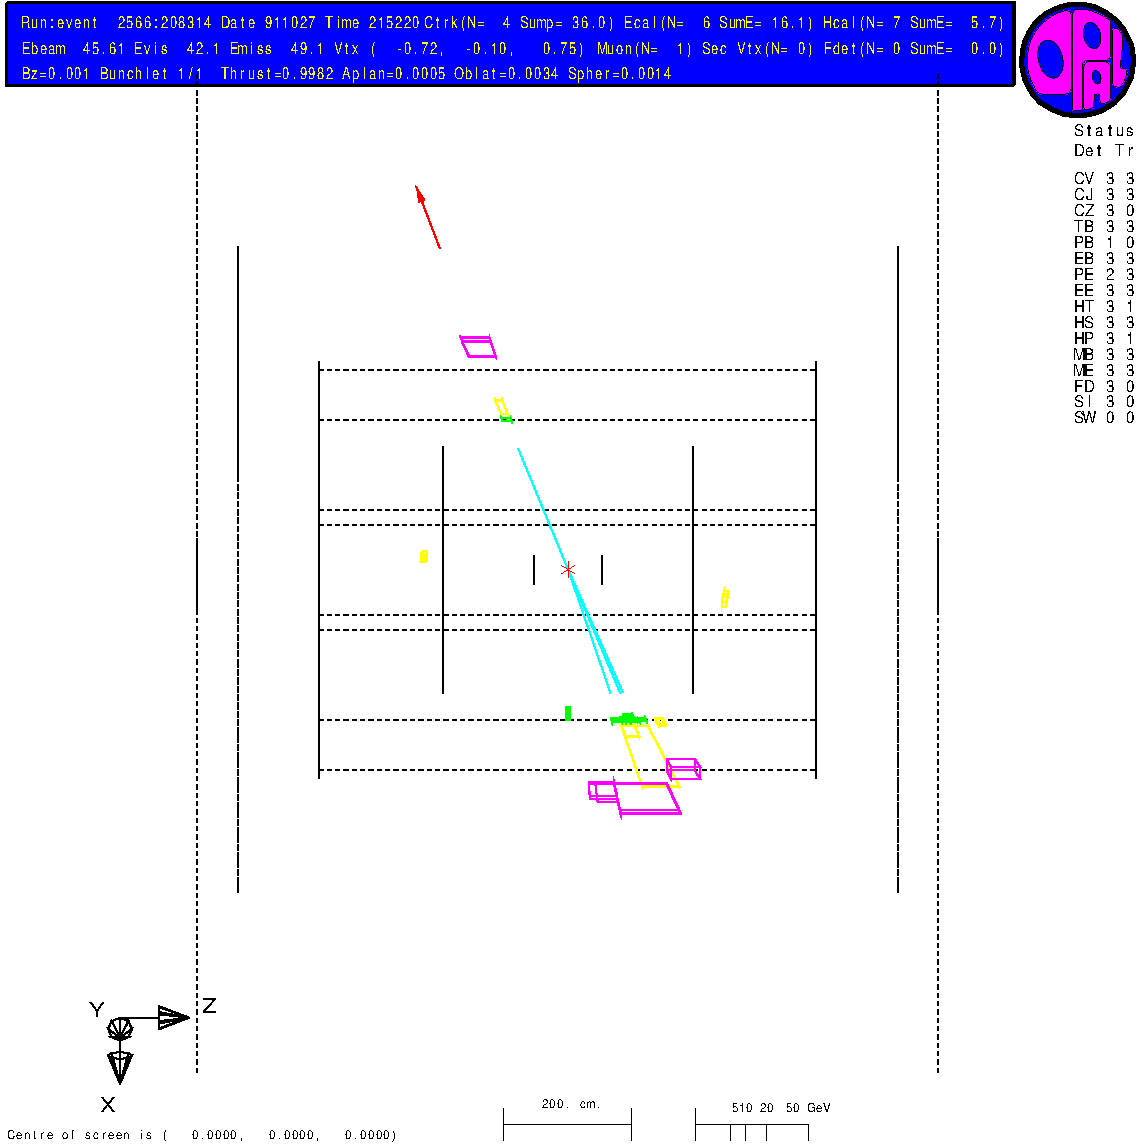
\includegraphics[width=.75\textwidth]{./data/tag1/tt_pics/cropped/tt_05_side}
		\subcaption{Side view}
	\end{subfigure}
	\caption{Exemplary picture of a $Z^0\rightarrow \tau^+\tau^-$ event. A 1-prong and a 3-prong is observable. The 1-prong event can be identified as a muon while the 3-prong consists of pions which are detected in the electromagnetic calorimeter (in case of $\pi^0$) and the hadronic calorimeter ($\pi^\pm$).}
\end{figure}
\clearpage
\subsubsection{Z$^0\rightarrow q\bar{q}$}

Decays of Z$^0$ into quark-antiquark pairs always produce jets where quarks hadronize to mesons or baryons.
Those can be identified as a large number of charged tracks in the tracking system.
In addition some of the hadrons decay into leptons which can be seen as signal in the electromagnetic calorimeter or the muon chambers.
The hadrons are stopped and seen as showers in the hadronic calorimeter.
\begin{sidewaystable}
	\centering
	\begin{tabular}{S[table-format=4.0]S[table-format=6.0]S[table-format=2.1]S[table-format=2.0]S[table-format=2.1]S[table-format=2.1]l}
	\toprule
	{Run} & {Event} & {\texttt{Ctrk(Sump)}} & {\texttt{Ctrk(N)}} & {\texttt{Ecal(SumE)}} & {\texttt{Hcal(SumE)}} & {Comments} \\
	\midrule
	2566 & 164184 & 37.7 & 15 & 37.0   & 14.1 & two jets with one muon each \\
	2566 & 195995 & 39.2 & 17 & 66.8 & 9.9  &  \\
	2566 & 196117 & 64.6 & 46 & 53.0   & 13.0   & low momentum particles on helical track \\
	2566 & 196548 & 33.3 & 8  & 67.5 & 13.3 & two jets with one muon each \\
	2568 & 78191  & 45.3 & 36 & 53.2 & 7.7  & \\
	2568 & 78425  & 59.9 & 41 & 53.2 & 13.8 & \\
	2568 & 78553  & 21.9 & 9  & 65.2 & 8.8  & \\
	2568 & 78787  & 55.9 & 16 & 50.4 & 24.3 & one jet containing a muon \\
	2568 & 79038  & 38.1 & 30 & 68.3 & 13.8 & three jets \\
	2568 & 79043  & 34.4 & 22 & 75.5 & 6.2  & \\
	2568 & 79181  & 51.2 & 36 & 62.3 & 5.5  & \\
	2568 & 79337  & 63.1 & 23 & 56.0   & 17.2 & \\
	2568 & 79487  & 59.0   & 23 & 60.6 & 8.5  & one jet containing a muon \\
	2568 & 79517  & 62.2 & 26 & 67.2 & 20.4 &  \\
	2568 & 79642  & 43.3 & 30 & 71.7 & 4.3  & three jets  \\
	2570 & 88252  & 47.8 & 40 & 61.4 & 5.7  & two jets with one muon each \\
	2570 & 88262  & 67.9 & 19 & 52.1 & 10.6 &  \\
	2570 & 88303  & 52.1 & 14 & 61.0   & 4.4  & \\
	2570 & 88328  & 82.6 & 29 & 53.8 & 16.4 & \\
	\bottomrule
\end{tabular}
	\caption{Collected data from the hadronic dataset. All values for energies and momenta in \si{GeV}. If unambiguously determinable, the number of jets is given.}
\end{sidewaystable}
\begin{figure}[h]
	\centering
	\begin{subfigure}{\textwidth}
		\centering
		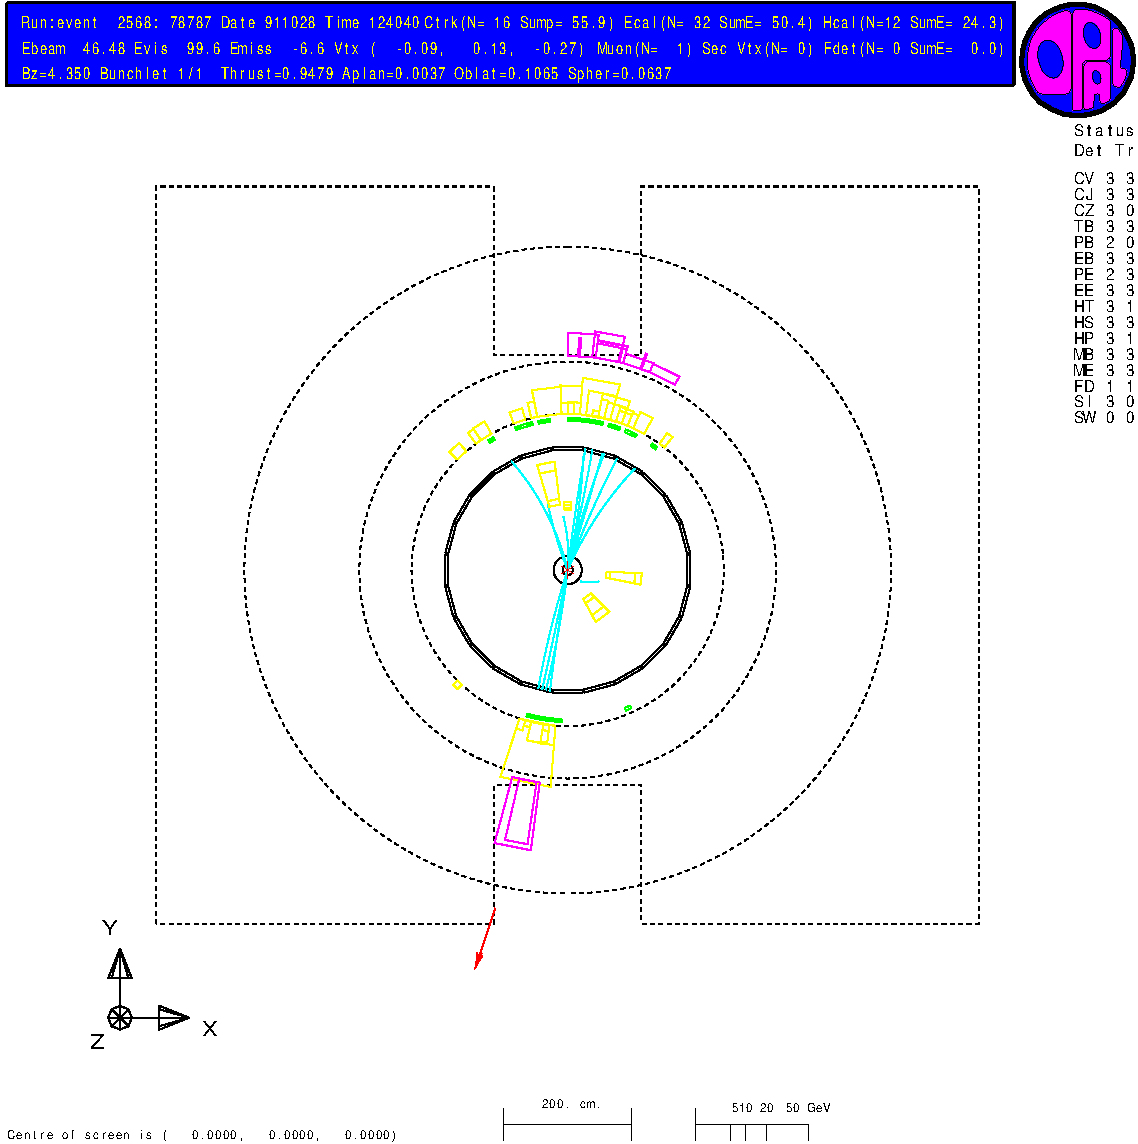
\includegraphics[width=.75\textwidth]{./data/tag1/qq_pics/cropped/qq_04}
		\subcaption{Front view}
	\end{subfigure}
	\begin{subfigure}{\textwidth}
		\centering
		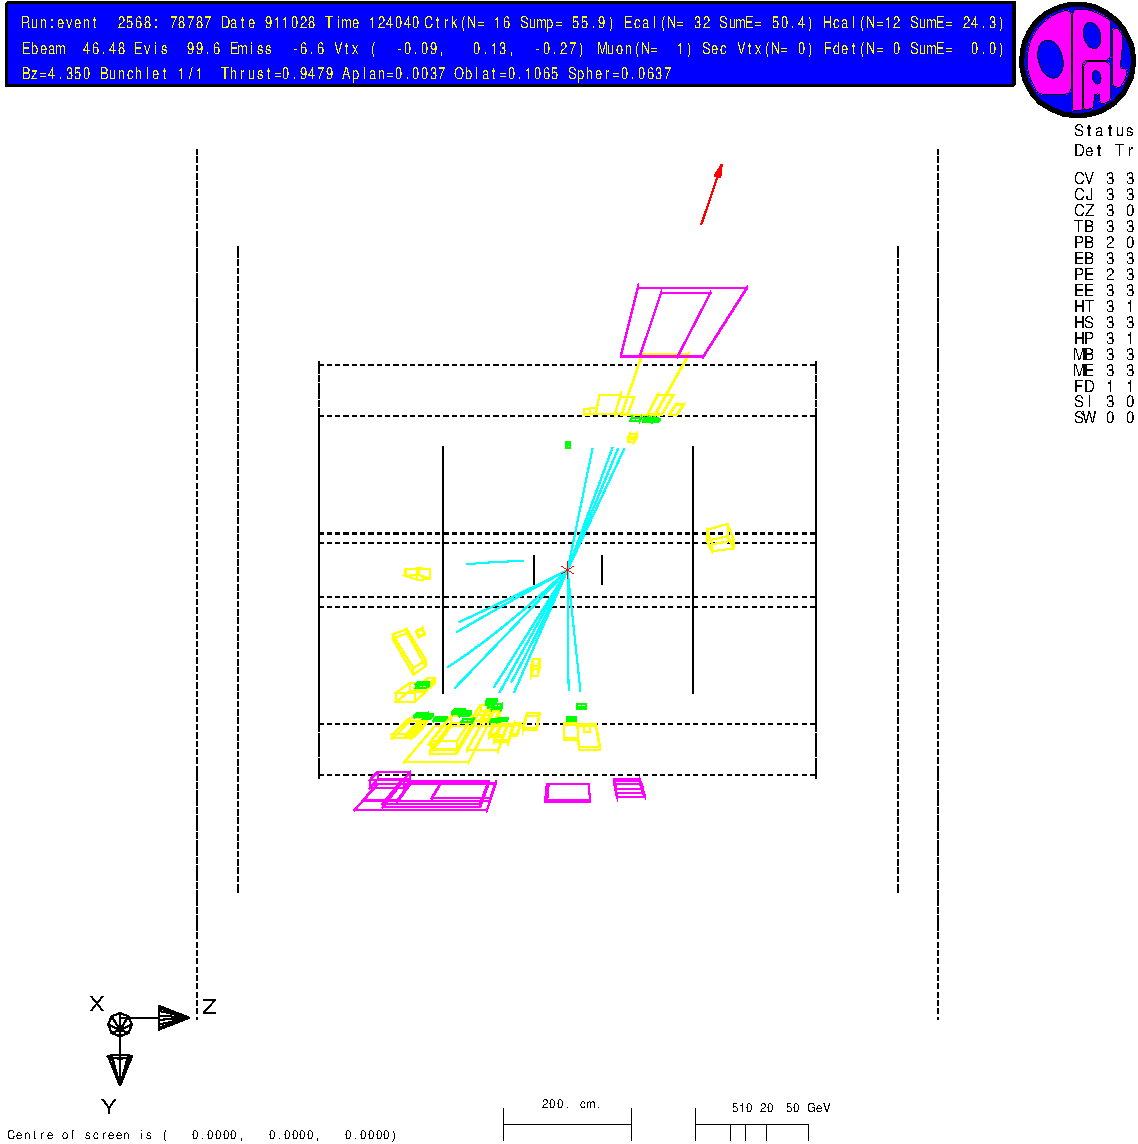
\includegraphics[width=.75\textwidth]{./data/tag1/qq_pics/cropped/qq_04_side}
		\subcaption{Side view}
	\end{subfigure}
	\caption{Exemplary picture of a $Z^0\rightarrow q\bar{q}$ event. One of the jets can be identified as a muonic event while the other tracks consist of electromagnetically interacting particles and hadrons.}
\end{figure}
\clearpage

\subsection{Event Identification in Test Sample}

Based on the observations from the previous exercise it was possible to evaluate cuts to apply on the data in order to distinguish between different decay channels of the Z boson.
Those are given by the parameters measured or reconstructed in the detector, Ctrk(N), Ctrk(SumP), Ecal(SumE) and Hcal(SumE).
In order to get optimal cut criteria, the data from all Monte-Carlo simulated samples has been histogrammed which is shown in figure \ref{fig:histograms}.
\begin{figure}[htb]
	\begin{subfigure}{.5\textwidth}
		\centering
		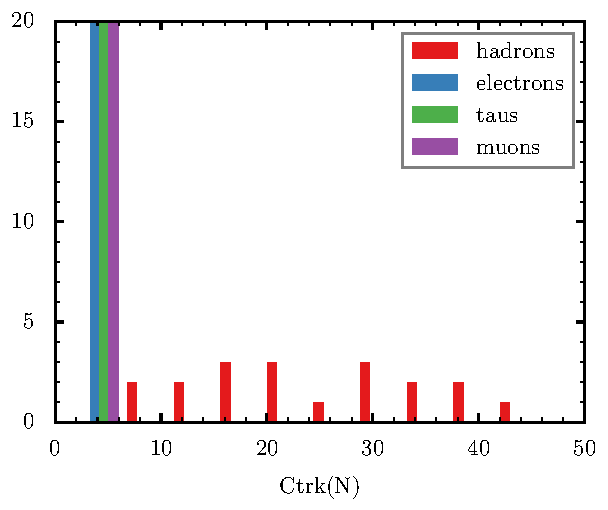
\includegraphics[width=\textwidth]{./figures/event_display/Ctrk(N)}

	\end{subfigure}
	\begin{subfigure}{.5\textwidth}
		\centering
		\includegraphics[width=\textwidth]{./figures/event_display/Ctrk(SumP)}

	\end{subfigure}
	\begin{subfigure}{.5\textwidth}
		\centering
		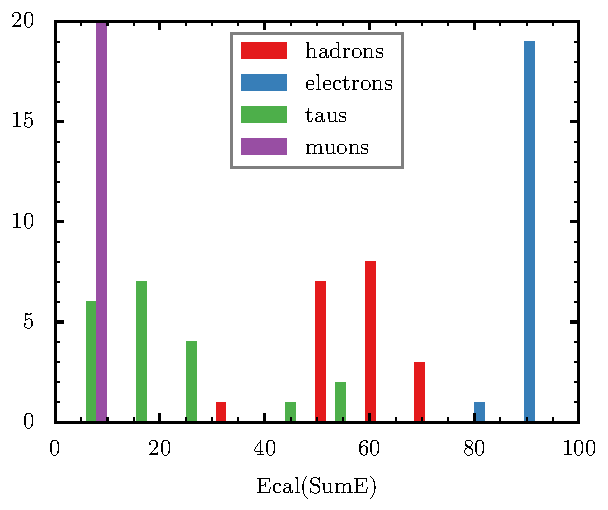
\includegraphics[width=\textwidth]{./figures/event_display/Ecal(SumE)}

	\end{subfigure}
	\begin{subfigure}{.5\textwidth}
		\centering
		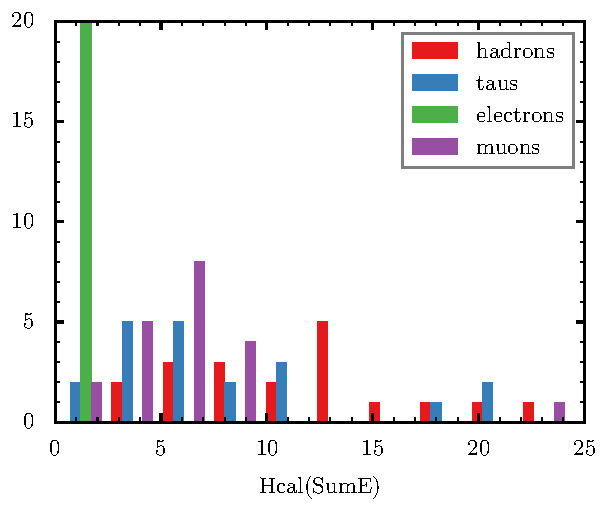
\includegraphics[width=\textwidth]{./figures/event_display/Hcal(SumE)}

	\end{subfigure}
	\caption{Distributions of the measured parameters for the different types of decay channels. To find cuts to differentiate between the decay channels the overlap of two distributions should be minimized without loosing two many events of the distribution of the particle type that shall be identified. All energies are given in \si{GeV}.}
	\label{fig:histograms}
\end{figure}
The used cuts are given in table \ref{tab:cut_criteria_day1} and can be reviewed by looking on the events in a test sample (dataset number 1 was used). 
Since all leptons produce mostly two or in case of the $\tau$ decay only a few charged particles this was a good possibility to distinguish decays where jets are formed from the leptonic ones.
Electrons are light, electromagnetically interacting particles and hence deposit all their energy in the electromagnetic calorimeter and no energy in the hadronic calorimeter which explains why we chose Ecal(SumE) to be larger than \SI{60}{GeV} and Hcal(SumE) to be smaller than \SI{2}{GeV}.
Muons lose only a small energy in the calorimeters, that is why those entries should be small compared to the measured momentum of the charged tracks.
To separate taus from muons and hadrons the momentum of all charged tracks could be used.
Since electrons and taus have nearly the same distribution for this variable a further separation is needed which can be done with the deposited energy in the electromagnetic calorimeter.
In general, since taus can decay to many different particles, they are difficult to identify by cuts.
All of the decay channels found with the cut criteria could be verified by analysis of event displays.
\begin{table}[htb]
	\centering
	\begin{tabular}{lcccc}
	\toprule
	 & $e$ & $\mu$ & $\tau$ & hadrons \\
	 \midrule
	\texttt{ncharged} & $< 5$  & $< 4$  & $< 8$ & $\geq 8$ \\
	\texttt{pcharged} & $> 30$ & $> 55$ & $>1\,\land\,<75$ & --\\
	\texttt{e\_ecal}  & $> 70$ & $< 15$  & $< 75$ & $> 20$ \\
	\texttt{e\_hcal}  & $< 15$  & $< 25$ & -- & -- \\
	\bottomrule
\end{tabular}
	\caption{Applied cuts on the data to identify the decay channel.}
	\label{tab:cut_criteria_day1}
\end{table}
\begin{sidewaystable}
	\centering
		\begin{tabular}{S[table-format=4.0]S[table-format=5.0]S[table-format=2.1]S[table-format=2.0]S[table-format=2.1]S[table-format=2.1]ll}
	\toprule
	{Run} & {Event} & {\texttt{Ctrk(Sump)}} & {\texttt{Ctrk(N)}} & {\texttt{Ecal(SumE)}} & {\texttt{Hcal(SumE)}} & ident.\ decay & Comments \\
	\midrule
4353 & 1080  & 39.5 & 19 & 44.3 & 15.6 & hadronic 		& two jets with one muon each \\
4353 & 2387  & 42.8 & 36 & 57.1 & 12.5 & hadronic 		& jets and one muon \\
4353 & 5386  & 95.7 & 2  & 93.4 & 0.0  & $e^+e^-$ 		& \\
4353 & 6057  & 90.8 & 2  & 1.4  & 4.1  & $\mu^+\mu^-$ 	& \\
4353 & 6696  & 36.5 & 4  & 35.8 & 10.8 & $\tau^+\tau^-$ & 1 and 3 prong \\
4353 & 7137  & 97.0 & 2  & 2.2  & 8.9  & $\mu^+\mu^-$   & possible cosmic background muon \\
4353 & 7219  & 42.9 & 68 & 48.5 & 6.2  & hadronic 		& \\
4353 & 8323  & 35.0 & 5  & 40.8 & 3.3  & $\tau^+\tau^-$ & muon and 3 prong, probably wrong reconstruction \\
4353 & 8641  & 75.8 & 21 & 45.8 & 21.0 & hadronic 		& two jets                                         \\
4353 & 9149  & 95.2 & 2  & 1.3  & 7.9  & $\mu^+\mu^-$   &                                                   \\
4353 & 9289  & 22.7 & 2  & 34.4 & 0.0  & $\tau^+\tau^-$ & 1 and 1 prong, considerable missing energy due to $\nu$\\
4353 & 9593  & 44.3 & 4  & 37.8 & 2.6  & $\tau^+\tau^-$ & 1 and 3 prong                                              \\
4353 & 9880  & 53.1 & 21 & 36.2 & 22.9 & hadronic 		&                                                   \\
4353 & 10900 & 89.5 & 2  & 92.0 & 0.0  & $e^+e^-$   	&                                                   \\
4353 & 11844 & 89.1 & 2  & 89.7 & 0.0  & $e^+e^-$    	&                                                   \\
4353 & 13556 & 4.1  & 2  & 4.4  & 0.0  & $\tau^+\tau^-$ & two-photon reaction (misidentification) \\
4353 & 14063 & 87.8 & 2  & 1.4  & 4.3  & $\mu^+\mu^-$   & \\
4353 & 14640 & 75.3 & 2  & 90.0 & 0.0  & $e^+e^-$    	& additional radiation losses \\
4353 & 14744 & 93.7 & 2  & 1.6  & 6.8  & $\mu^+\mu^-$   & \\
4353 & 15775 & 67.1 & 2  & 93.6 & 0.0  & $e^+e^-$    	& additional radiation losses \\
	\bottomrule
\end{tabular}
	\caption{Collected data from the events in the test sample dataset. The given decay channel is the classification based on the previously formulated cuts. All values for energies and momenta in \si{GeV}.}
\end{sidewaystable}

\clearpage
\section{Part II: Statistical Analysis of $\mathrm{Z}^0$ Decays}
The second part of this laboratory experiment is concerned with the analysis of data gathered by the OPAL-detector at LEP.
Since an analysis using event displays is infeasible, the data analysis software \texttt{PAW} is used instead.
The aim of this part is to determine the mass and (partial) decay width of the $\mathrm{Z}^0$ and in addition to this calculate the mixing~$\sin^2\theta_\mathrm{W}$ from the forward-backward asymmetry in the muon channel.

\subsection{Analysis of Monte-Carlo Data}
\label{sec:analysis_mc_data}
Before the data taken at the OPAL-detector can be evaluated, four datasets of Monte-Carlo data are analyzed to refine the preliminary cuts that were determined in the previous part.
These datasets contain a selection of simulated $\mathrm{Z}^0$ decays, which are separated into the different decay channels with electron, muon, tau or hadronic final states.
Since the number of simulated events is known, these datasets can be used to estimate the (mis-)identification probability of our final cuts.
The nomenclature that is used in describing the detector data is summarized in table~\ref{tab:desc_variables}.

\begin{table}[H]
	\centering
	\begin{tabularx}{0.9\textwidth}{lX}
		\toprule
		\textbf{Variable} & \textbf{Description} \\
		\midrule		
		\texttt{ncharged} & Number of charged particle tracks in the tracking detector \\
		\texttt{pcharged} & Total momentum of all charged particle tracks in the tracking detector \\
		\texttt{e\_ecal} & Total energy deposited in the electromagnetic calorimeter \\
		\texttt{e\_hcal} & Total energy deposited in the hadronic calorimeter \\
		\texttt{cos\_thet} & Angle between the incoming positron and outgoing positively charged particle (undefined if the number of positively charged particles in the final state is not equal to one) \\
		\texttt{e\_lep} & Beam energy at LEP \\
		\bottomrule
	\end{tabularx}
	\caption{Description of the variables in the $\mathrm{Z}^0$ decay datasets. Momenta and energies are always given in units of GeV.}
	\label{tab:desc_variables}
\end{table}

\subsubsection{Acceptance of the OPAL-Detector}
\label{sec:acceptance_detector}
To get accustomed to the data analysis software, the distributions of a number of variables in the MC-datasets were plotted as histograms.
One such variable is the sum of the charged particle momenta, which is depicted in figure \ref{fig:uncut_pcharged}.
\begin{figure}[h]
	\centering
	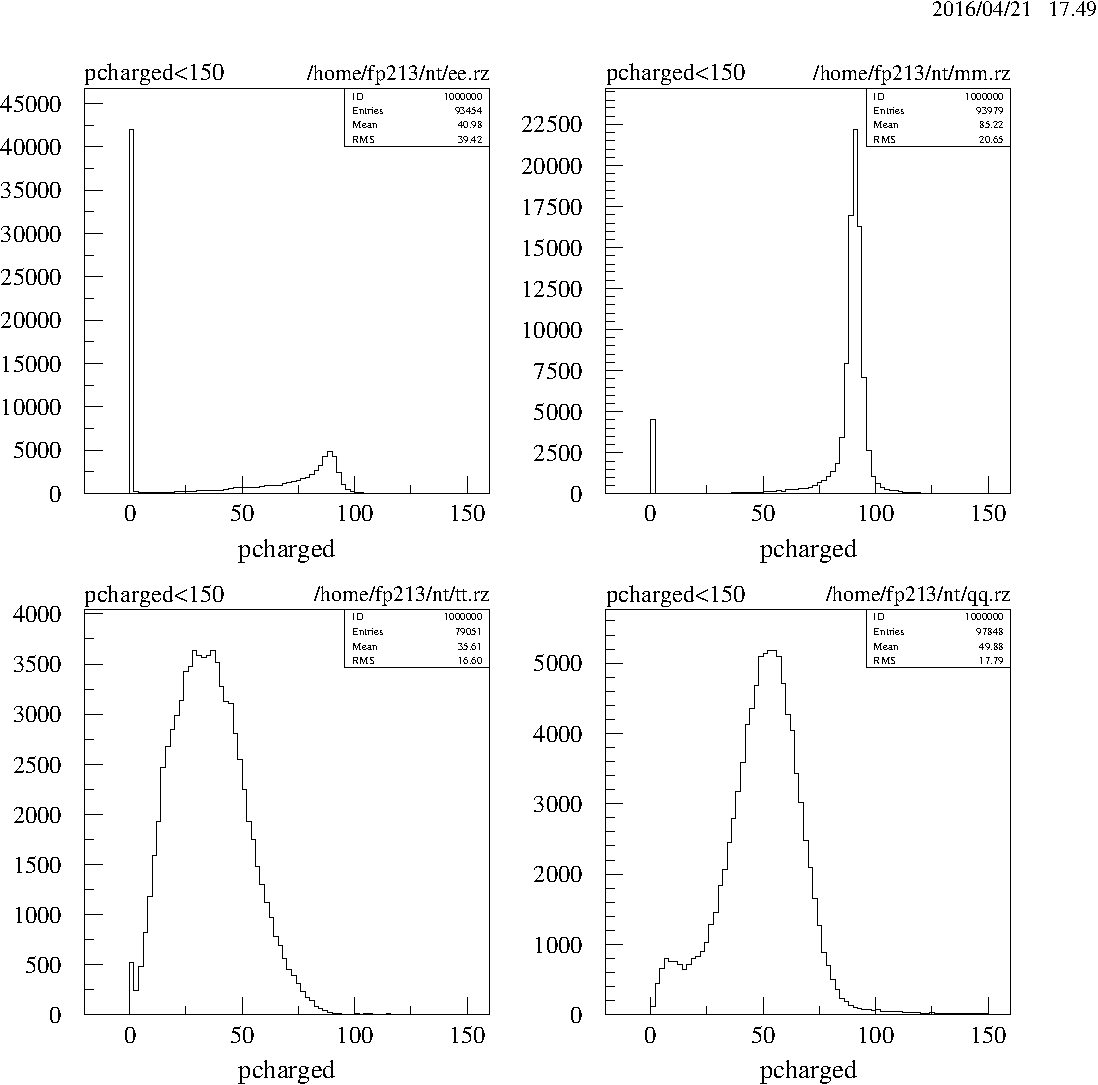
\includegraphics[width=1.0\textwidth]{./data/tag2/uncut/cropped/pcharged_uncut.pdf}
	\caption{Distribution of \texttt{pcharged} for the Monte-Carlo simulations of electron (upper left), muon (upper right), tau (lower left) and hadronic final states (lower right). The momenta are given in units of GeV.}
	\label{fig:uncut_pcharged}
\end{figure}
A notable feature of these distributions is the high number of events with vanishing \texttt{pcharged} for the electron and muon channel, which shall be analyzed further.
To investigate this occurrence additional cuts on other variables were performed, which lead to the observation that these events stem from particles that have been detected at very small angles with respect to the beam axis.
Since the detector cannot properly detect particles close to the beam axis, a cut on \texttt{cos\_thet} should decrease the number events with vanishing \texttt{pcharged}.
Therefore the cut
\begin{align*}
	\left| \cos\theta \right| < 0.9
\end{align*}
was chosen, which removed almost all events with vanishing \texttt{pcharged} in both channels.


\subsubsection{Refining the Cuts for Event Selection}
In order to optimize the cuts for event identification various variables of the simulated datasets have been plotted to allow for the determination of cut criteria to allow for the distinction of different decay channels of the Z-boson.
The histograms of the variables are depicted in appendix \ref{app:uncut_mc}.

Based on the observed distributions cuts on the parameters have been set, such that specific decay channels are filtered out of the datasets.
The cuts are chosen in a way, that a high number of events are retained while separating the different decay channels.
Nevertheless an optimal separation is not possible without discarding a high number of events, thus leading to diminished statistics.
Therefore in section~\ref{sec:efficiency_matrix} the number of misidentifications in the different decay channels is evaluated, leading to the formulation of a efficiency matrix.
Moreover in section~\ref{sec:s_t_channel_separation} additional cuts to the electron channel determined to separate $s$- and $t$-channel.
An overview of the selection cuts is given in table~\ref{tab:cut_criteria}, which were chosen according to the distribution of the various decay channels depicted in appendix~\ref{app:uncut_mc}.
\begin{table}[h]
	\centering
	\begin{tabular}{lcccc}
	\toprule
	 & $e$ & $\mu$ & $\tau$ & hadrons \\
	 \midrule
	\texttt{ncharged} & $< 5$  & $< 4$  & $< 8$ & $\geq 8$ \\
	\texttt{pcharged} & $> 30$ & $> 55$ & $>1\,\land\,<75$ & --\\
	\texttt{e\_ecal}  & $> 70$ & $< 15$  & $< 75$ & $> 20$ \\
	\texttt{e\_hcal}  & $< 15$  & $< 25$ & -- & -- \\
	\bottomrule
\end{tabular}
	\caption{Selection cuts for filtering of specific decay channels. A differentiation of $s$- and $t$-channel for the electron-channel is discussed in section~\ref{sec:s_t_channel_separation}.}
	\label{tab:cut_criteria}
\end{table}

\noindent In the following a short reasoning for the chosen cuts is given:
\begin{description}
	\item[Electron-channel] A cut in the number of charged particles is used to separate the electron from the hadron channel.
	Moreover a high energy deposition in the electromagnetic calorimeter is observed, so that a lower bound on the deposited energy leads to a good separation of the muon- and tau-channels.
	Finally additional cuts to the deposited energy in the hadronic calorimeter and the sum of charged particle momenta are applied, which further separate electrons from tau final-states.
	
	\item[Muon-channel] Again a cut in the number of charged particles separates the muon cleanly from the hadron-channel.
	An upper bound on the energy deposit in the electromagnetic calorimeter isolates it from the electron-channel and leads to some separation from the tau-channel.
	The cut on the sum of charged particle momenta leads to a clean separation from the tau-channel.	
	
	\item[Tau-channel] Again this channel is separated from the hadronic channel by the cut on \texttt{ncharged}.
	Moreover some separation of the electron and muon-channels is done by cutting on \texttt{e\_ecal} and \texttt{pcharged}.
	However the tau-channel is difficult to isolate from the remaining channels.
	Therefore a (relatively) high probability of misidentification of tau-events is expected.
	Quantitatively this is examined in section~\ref{sec:efficiency_matrix}. 
	
	\item[Hadron-channel] This channel is quite cleanly isolated by cutting on the number of charged particles due to the hadronization process.
	Nevertheless some misidentified tau-events can be expected.
\end{description}
In addition to these selection cuts the electron and muon-channels are cut in \texttt{cos\_thet} to remove non-reconstructible events close to the beam axis (according to section \ref{sec:acceptance_detector}).

\subsubsection{Separating $s$- and $t$-Channel in $\mathrm{e}^+ + \mathrm{e}^- \rightarrow \mathrm{e}^+ + \mathrm{e}^-$ Events}
\label{sec:s_t_channel_separation}
In section \korr{REF Vorbereitungsaufgaben} it was determined the differential cross section of the scattering process ($t$-channel) is strongly peaked in the forward direction.
This process only contributes marginally to the total differential cross section of $t$- and $s$-channel in the backward direction.
Therefore by constraining the scattering angle to larger values a selection of the annihilation process can be performed.
For the case of annihilation the contribution of the intermediate Z-boson to the cross section is dominant, at center of mass energies comparable to the Z-mass.

The angular distribution in the electron-channel is depicted in appendix~\ref{fig:cos_theta_uncut}, where one can clearly see the peak in the forward direction due to $t$-channel events.
To select the $s$-channel processes an upper bound on \texttt{cos\_thet} (scattering angle) is chosen, such that the angular distribution is mirror-symmetric with respect to $\cos\theta = 0$, reflecting the approximate\footnote{The forward-backward asymmetry is small compared to the asymmetry introduced by the $t$-channel process.} forward-backward symmetry of the $s$-channel process.

As the upper limit $\cos\theta < 0.5$ was chosen resulting in the angular distribution shown in figure~\ref{fig:t_cut_distribution}.
\begin{figure}[h]
	\centering
	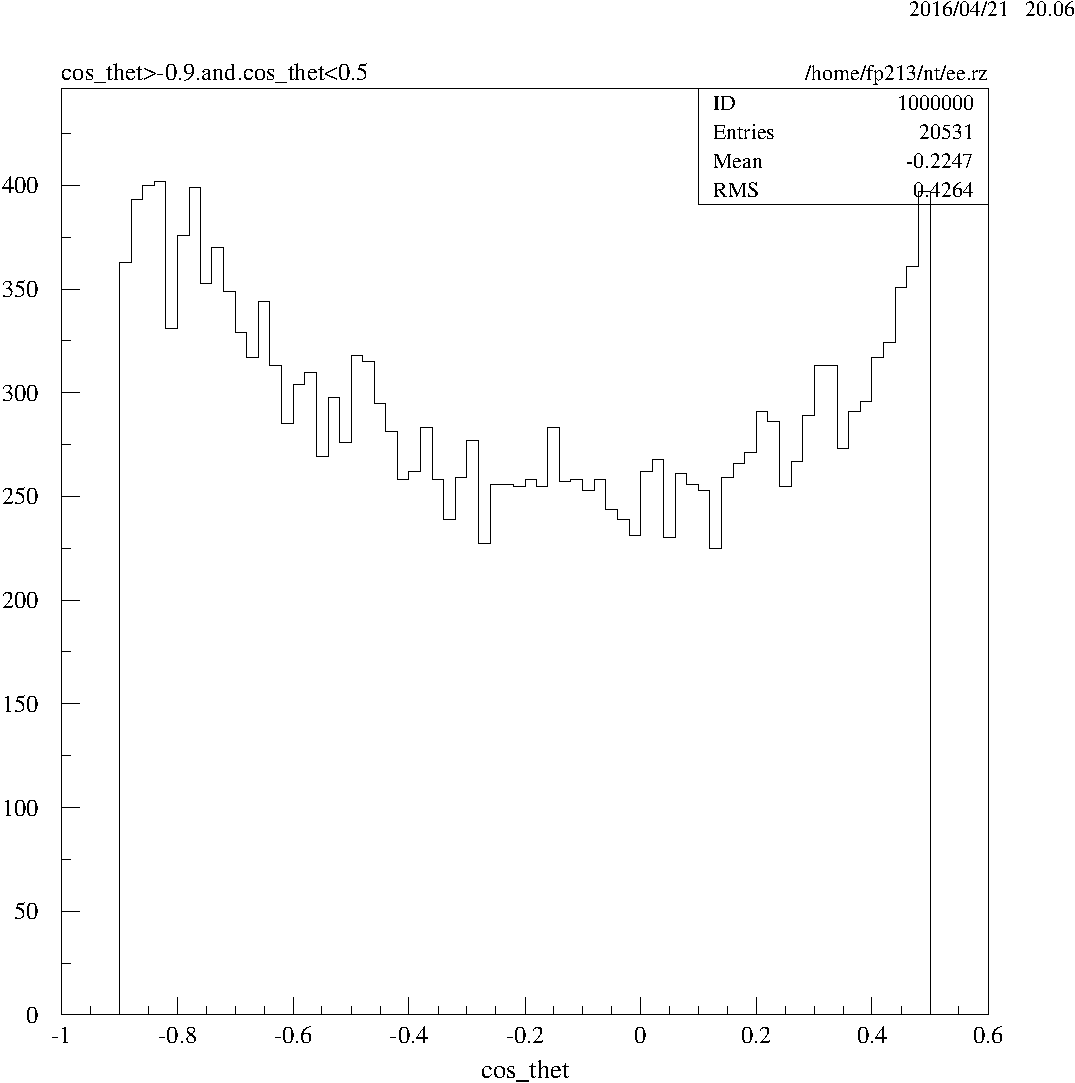
\includegraphics[width=0.8\textwidth]{./data/tag2/angular_mc/cropped/t_channel_cut.pdf}
	\caption{Angular distribution of the scattering angle in the electron-channel after separating $s$- and $t$-channel.}
	\label{fig:t_cut_distribution}
\end{figure}
In hindsight the chosen upper limit on the scattering angle was set too high, since the mirror-symmetry is clearly broken.
Therefore it is expected that there is a significant $t$-channel contribution in the final cuts, leading to a distortion of the measured resonance curve.

In addition to this the cut in the scattering angle leads to a significant loss of $s$-channel events in the forward direction.
Moreover the cut $\left| \cos\theta \right| < 0.9$ made in section~\ref{sec:acceptance_detector} also leads to some losses close to the beam pipe in the backward direction.
To correct for these losses one can consider that the differential cross-section of the $s$-channel process is given by
\begin{align*}
	\deriv{\sigma_\mathrm{s}}{\cos\theta} \propto \left( 1 + \cos\theta \right)
\end{align*}
thus the correction due to the cut on the scattering angle can be calculated by integration leading to
\begin{align*}
\kappa_\mathrm{angular} = \frac{\int_{-1}^{1}(1 + \cos^2\theta) \dinf{\cos\theta}}{\int_{-0.9}^{0.5}(1 + \cos^2\theta) \dinf{\cos\theta}} \approx 1.5829 \text{.}
\end{align*}
For the upcoming determination of the efficiency matrix it is important to know the total number of $s$-channel events in the MC-dataset, which contains $s$ as well as $t$-channel events.
Therefore one has to consider the total number of \num{100000} simulated events in the electron-channel ($s$- and $t$-channel) was reduced by a precut to \num{93454} events, discarding events that cannot be reconstructed.
Since the details of the precut are not known, it is assumed that it affects the $s$- and $t$-channel equally.
Thus the total number of annihilation events in the dataset can be calculated using
\begin{align*}
	N_\mathrm{e,\,s} = n_\mathrm{e,\,s} \cdot \frac{100000}{93454} \cdot \kappa_\mathrm{angular}
\end{align*}
with the number of $s$-channel events $n_\mathrm{e,\,s}$ after the cuts previously described.
Using the values in table~\ref{tab:num_events} the total number of $s$-channel events in the MC-dataset can be estimated to be
\begin{align*}
	N_\mathrm{e,\,s} = 34136
\end{align*}
which is used in section~\ref{sec:efficiency_matrix} to determine the efficiency matrix.

\begin{table}[h]
	\centering
	\begin{tabular}{rS[table-format=6.0]S[table-format=6.0]S[table-format=6.0]S[table-format=6.0]}
	\toprule
	&\multicolumn{4}{c}{dataset}  \\ \cmidrule(r){2-5}
	& {electrons} & {muons} & {tauons} & {hadrons}\\
	\midrule
	total & 100000 & 100000 & 100000 & 100000\\
	precut & 93454 & 93979 & 79051 & 97848\\
	$n_\mathrm{e}$ & 20229 & 0 & 692 & 6 \\
	$n_\mathrm{\mu}$ & 1 & 78537 & 4089 & 0 \\
	$n_\mathrm{\tau}$ & 117 & 549 & 76651 & 503 \\
	$n_\mathrm{q}$ & 0 & 0 & 934 & 97533 \\
 	\bottomrule
\end{tabular}
	\caption{Number of events in the various decay channels after applying the selection cuts described the previous sections on the MC-datasets. The plots for determining these values can be found in appendix~\ref{app:mc_final_cut}.}
	\label{tab:num_events}
\end{table}

\begin{description}
	\item[Remark] Applying the cut condition on a total of $N$ entries leads to $N$ binary decisions, whether the entry fulfills the cut or does not.
	Therefore the underlying statistical description is the binomial distribution, for which the standard deviation can be estimated by
	\begin{align*}
		\Delta n_i = \sqrt{N \cdot \left[ \frac{n_i}{N} - \left( \frac{n_i}{N} \right)^2 \right]} \quad \text{with}\quad i \in \{ \mathrm{e}, \mathrm{\mu}, \mathrm{\tau}, \mathrm{q} \} \,\text{,}
	\end{align*}
	where $n_i$ describes the number of events after cut $i$ and $N$ the total number of events.
	Therefore it is assumed that the standard deviations of event counts after cutting the data can be estimated by this statistic.
\end{description}


\subsubsection{Efficiency Matrix}
\label{sec:efficiency_matrix}
By setting cuts on the data one loses a fraction of the simulated events and in addition to this misidentification of events can occur.
Knowing that each datasets was simulated with \num{100000} events (or for the electron-channel the total number of events in the $s$-channel as determined in section~\ref{sec:s_t_channel_separation}) the efficiency of the event selection using cuts can be evaluated.
For this a matrix formalism is employed, which connects the number of events in the different decay channels (as determined by the cut selection) $\vec{n}$ with the number of events per channel in the underlying data $\vec{N}$.
This relation is described by the so called efficiency matrix~$E$
\begin{align*}
	E = \begin{pmatrix}
		E_{\mathrm{e e}} & E_{\mathrm{e \mu}} & E_{\mathrm{e \tau}} & E_{\mathrm{e q}} \\
		E_{\mathrm{\mu e}} & E_{\mathrm{\mu \mu}} & E_{\mathrm{\mu \tau}} & E_{\mathrm{\mu q}} \\
		E_{\mathrm{\tau e}} & E_{\mathrm{\tau \mu}} & E_{\mathrm{\tau \tau}} & E_{\mathrm{\tau q}} \\
		E_{\mathrm{q e}} & E_{\mathrm{q \mu}} & E_{\mathrm{q \tau}} & E_{\mathrm{q q}} \\
	\end{pmatrix}
\end{align*}
with matrix elements $E_{ij}$, which are defined by
\begin{align}
	E_{ij} = \frac{n_{ij}}{N_j} \quad \text{with} \quad i,j \in \{ \mathrm{e}, \mathrm{\mu}, \mathrm{\tau}, \mathrm{q} \}
	\label{eq:efficiency_matrix_elements}
\end{align}
with $n_{ij}$ the number of particles of type $j$ that were identified by the cut selection to be of type $i$ and the total number of simulated events of this type $N_j$.
According to this formalism the vector of identified particles $\vec{n} = (n_\mathrm{e}, n_\mathrm{\mu}, n_\mathrm{\tau}, n_\mathrm{q})^\mathrm{T}$ can be calculated from the efficiency matrix~$E$ and the vector containing the simulated events $\vec{N} = (N_\mathrm{e}, N_\mathrm{\mu}, N_\mathrm{\tau}, N_\mathrm{q})^\mathrm{T}$ by matrix multiplication
\begin{align}
	\vec{n} = E \cdot \vec{N} \,\text{.}
	\label{eq:efficiency_definition}
\end{align}
For ideal cuts the efficiency matrix would be the unit matrix, since the off-diagonal elements correspond to misidentification of the decay channel and the diagonal elements give the fraction of correctly identified events.

For real data the number of events in the different channels $\vec{N}$ is generally not known, but the different cuts can be applied to the data to obtain the vector of identified particles $\vec{n}$.
Then the number of events $\vec{N}$ in the different decay channels can be inferred from $\vec{n}$ using the inverse of equation \eqref{eq:efficiency_definition}
\begin{align}
	\vec{N} = E^{-1} \cdot \vec{n}
	\label{eq:efficiency_correction}
\end{align}
with the inverted efficiency matrix $E^{-1}$.

To calculate the efficiency matrix according to equation \eqref{eq:efficiency_matrix_elements} one has to note that $N_\mathrm{e}$ is not \num{100000} but rather the number of events in the s-channel as determined in section~\ref{sec:s_t_channel_separation}.
Using the number of events after the different cuts in table~\ref{tab:num_events} the matrix elements of the efficiency matrix can be calculated
\begin{align*}
	&E = \begin{pmatrix}
	0.59259 & 0.00001 & 0.00117 & 0.00000 \\
	0.00000 & 0.78537 & 0.00549 & 0.00000 \\
	0.02027 & 0.04089 & 0.76651 & 0.00934 \\
	0.00018 & 0.00000 & 0.00503 & 0.97533 \\
	\end{pmatrix}
\end{align*}
and the errors are calculated by first order error propagation using the standard deviation as estimated by the underlying binomial distribution for the number of events after cutting
\begin{align*}
	&\Delta E = \begin{pmatrix}
	0.00266 & 0.00000 & 0.00000 & 0.00000 \\
	0.00000 & 0.00130 & 0.00024 & 0.00000 \\
	0.00077 & 0.00063 & 0.00134 & 0.00031 \\
	0.00008 & 0.00000 & 0.00023 & 0.00050 \\
	\end{pmatrix} \,\text{.}
\end{align*}
The off-diagonal elements of this matrix are almost zero meaning that the probability of misidentification is small.
The largest off-diagonal elements with misidentification probabilities of the order of $1 \%$ are the elements for tau-events misidentified as either electron- or muon-events.
This is because separating tau-events from those channels is rather difficult as was mentioned previously.
Moreover the diagonal elements give the fraction of correctly identified events.
Due to the clear signature of hadronic events almost $100 \%$ of events are identified correctly.
For the muon- and tau-channel larger losses of the order of $20 \%$ are observed.
The smallest efficiency of $60 \%$ is observed for the electron-channel due to the high number of discarded events caused by the angular cuts.

For the further analysis the efficiency matrix has to be inverted.
Since the analytical error propagation in the process of inverting this matrix is rather complicated, a Monte-Carlo approach was used instead.
For this a random sample of $\num{100000}$ different efficiency matrices was generated according to the standard deviations given in the error matrix.
The sampled matrices can then be inverted using a numerical algorithm and a sample of $\num{100000}$ inverted efficiency matrices is generated.
From the samples of the inverse matrix the error of the matrix elements can be estimated by the sample standard deviation.
Finally the resulting inverted matrix is given by
\begin{align*}
&E^{-1} = \begin{pmatrix}
	1.68758 & 0.00011 &-0.00258 & 0.00002 \\
	0.00312 & 1.27376 &-0.00912 & 0.00009 \\
   -0.04465 &-0.06796 & 1.30525 &-0.01250 \\
   -0.00007 & 0.00035 &-0.00673 & 1.02536 \\
\end{pmatrix}
\end{align*}
with the error matrix by Monte-Carlo error propagation
\begin{align*}
&\Delta E^{-1} = \begin{pmatrix}
	0.00756 & 0.00001 & 0.00002 & 0.00001 \\
	0.00002 & 0.00211 & 0.00039 & 0.00001 \\
	0.00170 & 0.00105 & 0.00227 & 0.00041 \\
	0.00013 & 0.00002 & 0.00030 & 0.00052 \\
\end{pmatrix} \,\text{.}
\end{align*}
In the following this matrix can be used in analyzing real data gathered at OPAL.

\subsection{Analysis of OPAL-Data}
After the analysis of the cuts for event selection was performed, the data measured at the OPAL-detector can be analyzed.
Of the available datasets \texttt{data6} was chosen, since it has the highest integrated luminosities and therefore should allow for better statistics.

The dataset contains events at seven different center of mass energies at LEP surrounding the Z-resonance.
Therefore in a first step the measurement at different energies have to be separated by a cut in \texttt{e\_lep}.
In the following only the mean value of the center of mass energy is denoted, since the energies vary only slightly from this value.

\subsubsection{Determination of the Cross Section}
\label{sec:determination_cross_section}
After the energies have been separated the selection cuts can be applied to the samples at different energies $\sqrt{s}$.
From these the remaining number of particles $n_i$ with $i \in \{ \mathrm{e}, \mathrm{\mu}, \mathrm{\tau}, \mathrm{q} \}$ can be obtained.
The number of events after the cuts is summarized in table \ref{tab:counts_cross_section}.
To obtain the total number of events of a specific type one has to correct for the efficiency of the cut selection.
This is simply done by matrix multiplication of the inverse efficiency matrix $E^{-1}$ as in equation \eqref{eq:efficiency_correction} with the vector $\vec{n}$.
The error of the correction counts can be calculated using first order error propagation:
\begin{align}
&\Delta N_i = \sqrt{\sum_k \left[ n_k^2 \cdot \left(\Delta E^{-1}\right)_{ik}^2 + \left(E^{-1}\right)_{ik}^2 \cdot \Delta n_k^2 \right]} \,\text{.}
\label{eq:error_prop_matrix_mult}
\end{align}
The efficiency corrected number of events are summarized in table \ref{tab:counts_cross_section_corr}.

\begin{table}
	\begin{subtable}{1.0\textwidth}
		\centering
		\begin{tabular}{S[table-format=2.2]S[table-format=4.0,table-figures-uncertainty=3]S[table-format=4.0,table-figures-uncertainty=3]S[table-format=5.0,table-figures-uncertainty=3]S[table-format=6.0,table-figures-uncertainty=3]}
	\toprule
	{$\sqrt{s}$ / \si{GeV}} & {$n_\mathrm{e}$} & {$n_\mathrm{\mu}$} & {$n_\mathrm{\tau}$} & {$n_\mathrm{q}$}\\
	\midrule
	88.48 & 126 +- 12 & 124 +- 12 & 236 +- 16 & 3527 +- 39 \\
	89.47 & 303 +- 18 & 310 +- 18 & 454 +- 21 & 7904 +- 51 \\
	90.23 & 502 +- 23 & 611 +- 25 & 787 +- 28 & 15629 +- 61 \\
	91.24 & 6273 +- 79 & 8980 +- 94 & 12055 +- 108 & 234605 +- 211 \\
	91.96 & 490 +- 22 & 790 +- 28 & 1049 +- 32 & 19868 +- 62 \\
	92.97 & 182 +- 14 & 301 +- 18 & 484 +- 22 & 8604 +- 45 \\
	93.72 & 216 +- 15 & 353 +- 19 & 493 +- 22 & 9156 +- 50 \\
	\bottomrule
	
\end{tabular}
		\subcaption{Number of events at the specified center of mass energy $\sqrt{s}$ after applying the cut selection. The error is estimated from binomial statistics.}
		\label{tab:counts_cross_section}
	\end{subtable}
	
	\vspace{0.5cm}
	
	\begin{subtable}{1.0\textwidth}
		\centering
		\begin{tabular}{S[table-format=2.2]S[table-format=5.0,table-figures-uncertainty=3]S[table-format=5.0,table-figures-uncertainty=3]S[table-format=5.0,table-figures-uncertainty=3]S[table-format=6.0,table-figures-uncertainty=3]}
	\toprule
	{$\sqrt{s}$ / \si{GeV}} & {$N_\mathrm{e}$} & {$N_\mathrm{\mu}$} & {$N_\mathrm{\tau}$} & {$N_\mathrm{q}$}\\
	\midrule
	88.48 & 212 +- 19 & 156 +- 15 & 250 +- 20 & 3615 +- 40 \\
	89.47 & 510 +- 30 & 392 +- 23 & 459 +- 28 & 8101 +- 53 \\
	90.23 & 846 +- 38 & 773 +- 32 & 768 +- 37 & 16020 +- 63 \\
	91.24 & 10562 +- 141 & 11351 +- 121 & 11912 +- 173 & 240476 +- 248 \\
	91.96 & 825 +- 38 & 999 +- 36 & 1045 +- 43 & 20365 +- 65 \\
	92.97 & 306 +- 23 & 380 +- 22 & 496 +- 29 & 8819 +- 46 \\
	93.72 & 364 +- 25 & 446 +- 24 & 495 +- 29 & 9385 +- 51 \\
	\bottomrule
	
\end{tabular}
		\subcaption{Total number of events after correction for the efficiency of the cut selection. The error is estimated by first order error propagation as given in equation \eqref{eq:error_prop_matrix_mult}.}
		\label{tab:counts_cross_section_corr}
	\end{subtable}
	\caption{Number of events at center of mass energies $\sqrt{s}$ near the Z-resonance given by the selection cuts determined in section \ref{sec:analysis_mc_data}.}
\end{table}

After the total number of events has been determined, the cross section can be calculated at the different center of mass energies.
For this the relation
\begin{align*}
	N_i = \sigma_i \cdot \int \mathcal{L} \dinf{t}
\end{align*}
can be used to determine the cross section from the number of events at a specific energy and the integrated luminosity in the specified energy interval.
This can be solved for the cross section thus obtaining
\begin{align*}
	\sigma_i = \frac{N_i}{\int \mathcal{L} \dinf{t}} \, \text{.}
\end{align*}
Moreover radiation corrections to the cross section are necessary, so that the cross section can be calculated by
\begin{align*}
	\sigma_i = \frac{N_i}{\int \mathcal{L} \dinf{t}} + \mathrm{corr}_i(\sqrt{s}) \,\text{.}
\end{align*}
Using the integrated luminosities for the given dataset (\texttt{data6}) and the radiation correction summarized in table~\ref{tab:lumi_corr} the cross sections can be calculated.
\begin{table}[h]
	\centering
	\begin{tabular}{S[table-format=2.5]S[table-format=4.4,table-figures-uncertainty=4]S[table-format=1.2,retain-explicit-plus]S[table-format=2.2,retain-explicit-plus]}
	\toprule
	&&\multicolumn{2}{c}{$\mathrm{corr}_i(\sqrt{s})$ / nb}\\
	\cmidrule{3-4}
	{$\sqrt{s}$ /  GeV} & {$\int \mathcal{L} \dinf{t}$ / \si{\per\nano\barn}} & {leptons} & {hadrons} \\
	\midrule
	88.48021 & 675.8590 +- 5.7213 & +0.09 & +2.0 \\
	89.46928 & 800.8436 +- 6.6065 & +0.20 & +4.3 \\
	90.22604 & 873.7021 +- 7.1212 & +0.36 & +7.7 \\
	91.24186 & 7893.498 +- 54.307 & +0.52 & +10.8 \\
	91.96859 & 825.2780 +- 6.8530 & +0.22 & +4.7 \\
	92.96836 & 624.5900 +- 5.5009 & -0.01 & -0.2 \\
	93.71685 & 942.2280 +- 7.7043 & -1.6 & -0.08 \\
	\bottomrule
\end{tabular}
	\caption{Integrated luminosities at LEP for the given center of mass energy from \cite{anleitung} and radiation correction to the cross section as given in \cite{instructions}.}
	\label{tab:lumi_corr}
\end{table}
The calculated cross sections at the specified center of mass energies are summarized in table~\ref{tab:cross_sections} using first order error propagation.
\begin{table}[h]
	\centering
	\begin{tabular}{S[table-format=2.2]S[table-format=1.3,table-figures-uncertainty=4]S[table-format=1.3,table-figures-uncertainty=4]S[table-format=1.3,table-figures-uncertainty=4]S[table-format=2.3,table-figures-uncertainty=4]}
	\toprule
	{$\sqrt{s}$ / \si{GeV}} & {$\sigma_\mathrm{e}$ / \si{nb}} & {$\sigma_\mathrm{\mu}$ / \si{nb}} & {$\sigma_\mathrm{\tau}$ / \si{nb}} & {$\sigma_\mathrm{q}$ / \si{nb}}\\
	\midrule
	88.48 & 0.404 +- 0.028 & 0.321 +- 0.021 & 0.460 +- 0.030 & 7.349 +- 0.075\\
	89.47 & 0.837 +- 0.037 & 0.689 +- 0.028 & 0.773 +- 0.035 & 14.416 +- 0.106 \\
	90.23 & 1.326 +- 0.044 & 1.244 +- 0.037 & 1.239 +- 0.043 & 26.036 +- 0.166 \\
	91.24 & 1.858 +- 0.021 & 1.958 +- 0.019 & 2.029 +- 0.025 & 41.265 +- 0.212 \\
	91.96 & 1.219 +- 0.046 & 1.430 +- 0.044 & 1.487 +- 0.053 & 29.377 +- 0.220 \\
	92.97 & 0.480 +- 0.037 & 0.598 +- 0.036 & 0.784 +- 0.046 & 13.920 +- 0.145 \\
	93.72 & 0.306 +- 0.027 & 0.393 +- 0.026 & 0.446 +- 0.031 & 8.360 +- 0.098 \\
	\bottomrule
	
\end{tabular}
	\caption{Calculated cross sections of the different decay channels using the measured number of events in table~\ref{tab:counts_cross_section_corr} and the integrated luminosities as well as radiation corrections given in table~\ref{tab:lumi_corr}. The errors are calculated using first order error propagation.}
	\label{tab:cross_sections}
\end{table}
These results are discussed in detail in the upcoming sections.

\subsubsection{Determination of the Forward-Backward Asymmetry using Muons}
The Weinberg angle can be determined from the forward-backward asymmetry of the decay $\mathrm{Z}^0 \rightarrow \mu^- \mu^+$, that is the asymmetry in the number of positively charged muons in the forward direction $n_\mathrm{F}$ compared to positively charged muons in the backward direction $n_\mathrm{B}$.
The asymmetry can be calculated using
\begin{align*}
	A_\mathrm{FB} = \frac{n_\mathrm{F} - n_\mathrm{B}}{n_\mathrm{F} + n_\mathrm{B}} + \mathrm{corr}(\sqrt{s})
\end{align*}
including a radiation correction $\mathrm{corr}(\sqrt{s})$.
For calculating the forward-backward asymmetry no efficiency correction has to be performed, since the correction cancels in the resulting expression.
Using the previously determined cut for muon-event selection the forward-backward asymmetry can be measured using the additional cuts 
\begin{align*}
	&\cos\theta > 0 \quad \text{(forward direction)} \\
	&\cos\theta < 0 \quad \text{(backward direction)}
\end{align*}
thus obtaining $n_\mathrm{F}$ or $n_\mathrm{B}$ respectively.
In table \ref{tab:afb} the number of events in forward/backward direction, as well as the calculated forward-backward asymmetry $A_\mathrm{FB}$ have been summarized.
\begin{table}[h]
	\centering
	\begin{tabular}{S[table-format=2.2]S[table-format=4.0,table-figures-uncertainty=2]S[table-format=4.0,table-figures-uncertainty=3]S[table-format=0.6]@{\hskip 2em}S[table-format=1.4,table-figures-uncertainty=4]}
		\toprule
		{$\sqrt{s}$ / \si{GeV}} & {$n_\mathrm{F}$} & {$n_\mathrm{B}$} & {$\mathrm{corr}(\sqrt{s})$} & {$A_\mathrm{FB}$} \\
		\midrule
		88.48 & 52 +- 6 & 72 +- 6 & 0.021512 & -0.1398 +- 0.0635\\
		89.47 & 149 +- 9 & 161 +- 9 & 0.019262 & -0.0195 +- 0.0402 \\
		90.23 & 279 +- 13 & 332 +- 13 & 0.016713 & -0.0700 +- 0.0287 \\
		91.24 & 4457 +- 48 & 4523 +- 48 & 0.018293 & 0.0119 +- 0.0075 \\
		91.96 & 397 +- 15 & 393 +- 15 & 0.030286 & 0.0353 +- 0.0252 \\
		92.97 & 176 +- 9 & 125 +- 9 & 0.062196 & 0.2316 +- 0.0408 \\
		93.72 & 196 +- 10 & 157 +- 10 &0.093850 & 0.2043 +- 0.0377 \\
		\bottomrule
\end{tabular}

	\caption{Number of events in the forward $n_\mathrm{F}$ and backward direction $n_\mathrm{B}$, radiation correction to the forward-backward asymmetry $\mathrm{corr}(\sqrt{s})$ as given in \cite{anleitung} and the corrected forward-backward asymmetry $A_\mathrm{FB}$. The errors for the number of events is given by binomial statistics and the error of the forward-backward asymmetry by first order error propagation.}
	\label{tab:afb}
\end{table}
\begin{figure}[h]
	\centering
	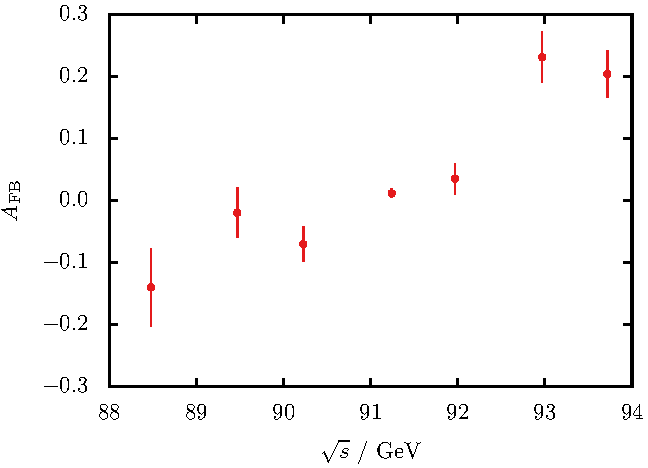
\includegraphics{./figures/afb.pdf}
	\caption{Measured forward-backward asymmetry~$A_\mathrm{FB}$ in the muon-channel for seven different center of mass energies~$\sqrt{s}$ (cf. table~\ref{tab:afb}).}
\end{figure}


The forward-backward asymmetry at the peak of the resonance can be approximated by \cite{instructions}
\begin{align*}
	A_\mathrm{FB}^\mathrm{peak} \approx 3 \left( 1 - 4 \sin^2\theta_\mathrm{W} \right)
\end{align*}
with the Weinberg mixing angle $\theta_\mathrm{W}$.
This can be approximated by the value measured at a center of mass energy of $\sqrt{s} = \SI{91.24}{GeV}$
\begin{align*}
	A_\mathrm{FB}^\mathrm{peak} \approx \num{0.0119 +- 0.0075}
\end{align*}
thus allowing the calculation of $\sin^2\theta_\mathrm{W}$ using
\begin{align*}
	\sin^2\theta_\mathrm{W} = \frac{1 - \sqrt{A_\mathrm{FB}^\mathrm{peak} / 3}}{4} \,\text{.}
\end{align*}
From this approximation the Weinberg angle can be estimated to be
\begin{align*}
	\sin^2\theta_\mathrm{W} = \num{0.234 +- 0.005}
\end{align*}
using first order error propagation.
The value calculated by using the forward-backward asymmetry is in good agreement with the literature value of \cite{pdg}
\begin{align*}
	(\sin^2\theta_\mathrm{W})^\mathrm{PDG} = \num{0.23126(5)} \,\text{.}
\end{align*}


\subsubsection{Fitting of a Breit-Wigner Distribution}
\label{sec:fit_resonance}
From the cross sections that were determined in section~\ref{sec:determination_cross_section} various quantities can be extracted by fitting a resonance curve.
For center of mass energies~$E_\mathrm{cm}$ close to the Z-boson mass the resonance can be described by a Breit-Wigner distribution given by
\begin{align}
	\sigma(E_\mathrm{cm}; A, M_\mathrm{Z}, \Gamma_\mathrm{Z}) = \frac{A}{2\pi} \frac{\Gamma_\mathrm{Z}}{(E_\mathrm{cm} - M_\mathrm{Z})^2 + \Gamma_\mathrm{Z}^2 / 4}
	\label{eq:breit_wigner}
\end{align}
with parameters $A$ proportional to the amplitude of the resonance, the mass of the Z-boson $M_\mathrm{Z}$ and the full decay width~$\Gamma_\mathrm{Z}$.
By fitting this distribution to the measured cross sections in table~\ref{tab:cross_sections} a number of parameters can be extracted, namely the mass~$M_\mathrm{Z}$, the full decay width~$\Gamma_\mathrm{Z}$ and the cross section at peak
\begin{align}
	\sigma^\mathrm{peak} = \frac{2A}{\pi \Gamma_\mathrm{Z}} \,\text{.}
	\label{eq:peak_cross_section}
\end{align}
The fitting of the Breit-Wigner distribution was done using a non-linear least squares algorithm \cite{lmfit} and the plots of the calculated cross sections as well as the fitted distributions for the different decay channels are depicted in figure~\ref{fig:cross_section_fit}.
\begin{table}[h]
	\centering
	\begin{tabular}{lS[table-format=2.2,table-figures-uncertainty=3]S[table-format=1.2,table-figures-uncertainty=3]S[table-format=2.3,table-figures-uncertainty=4]S[table-format=1.3]}
	\toprule
	{}& {$M_\mathrm{Z}$ / GeV} & {$\Gamma_\mathrm{Z}$ / GeV} & {$\sigma^\mathrm{peak}$ / nb} & {$\chi_\mathrm{red}^2$} \\
	\midrule
	electrons & 90.99 +- 0.24 & 2.47 +- 0.11 & 1.934 +- 0.077 & 2.796 \\
	muons & 91.18 +- 0.12 & 2.47 +- 0.05 & 1.966 +- 0.033 & 0.847 \\
	tauons & 91.22 +- 0.26 & 2.72 +- 0.10 & 2.015 +- 0.069 & 2.451 \\
	hadrons & 91.19 +- 0.70 & 2.53 +- 0.02 & 41.138 +- 0.270 & 1.776 \\	
	\midrule
	mean & 91.15 +- 0.10 & 2.52 +- 0.02 & {--} & {--} \\
	\bottomrule	
\end{tabular}
	\caption{Quantities extracted from the fit at the cross section data of the different decay channels.}
	\label{tab:fit_params}
\end{table}
Furthermore the quantities resulting from the best-fit (i.e.\ the mass~$M_\mathrm{Z}$, full decay width~$\Gamma_\mathrm{Z}$ and peak cross section~$\sigma^\mathrm{peak}$) and the reduced $\chi^2$ are summarized in table~\ref{tab:fit_params}.
In calculating the peak cross section from the fit parameters according to equation~\eqref{eq:peak_cross_section} the correlations of the fit-errors are considered in first order error propagation.
\begin{figure}[tb]
	\centering
	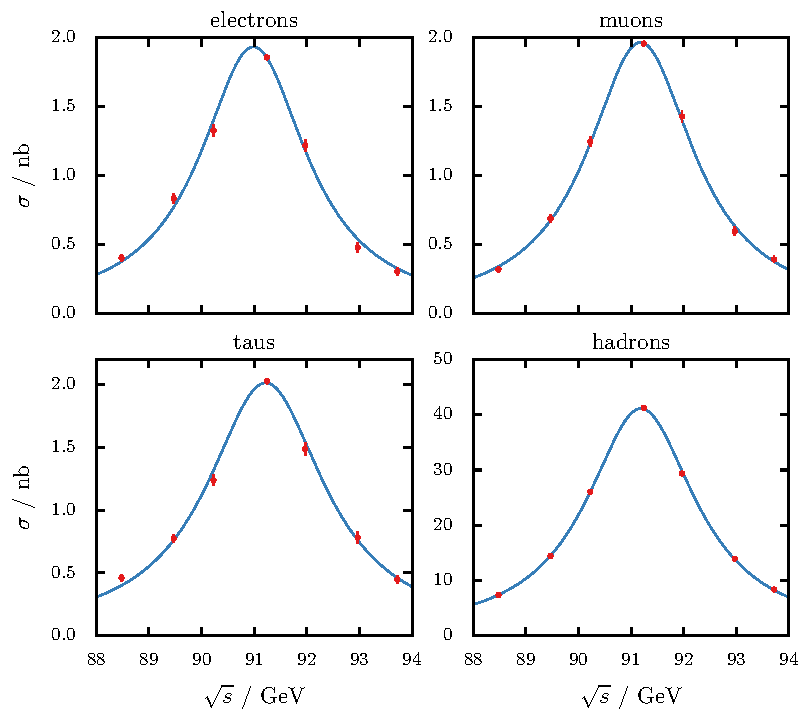
\includegraphics{./figures/cross_sections.pdf}
	\caption{Measured cross sections for the different decay channels (cf.\ table~\ref{tab:cross_sections}) and fitted Breit-Wigner distributions as given in equation \eqref{eq:breit_wigner}. The resulting fit parameters of the best-fit are summarized in table~\ref{tab:fit_params}.}
	\label{fig:cross_section_fit}
\end{figure}

In the following the results of the least-squares fits are discussed.
The electron channel shows a rather large deviation from the expected mass of the Z-boson and a large reduced $\chi^2$.
This is due to the the fact that still a significant part of $t$-channel events is contained in the dataset as was discussed in section~\ref{sec:s_t_channel_separation}, thus leading to a distortion of the resulting distribution and therefore to a lower observed mass.
Nevertheless the full decay width seems to be unaffected by the additional $t$-channel events.
Moreover a large $\chi_\mathrm{red}^2$ and a large deviation from the expected decay width is observed for the tau channel.
The reason for this observation is probably that the differentiation of the tau channel from the other channels by using selection cuts is difficult and misidentifications cannot be fully resolved by the efficiency correction.
This could probably be improved by using more sophisticated cuts for the tau channel.
The muon and the hadron channel fit well with the calculated cross sections with reduced $\chi^2$ close to one.
An additional discussion with respect to the confidence levels of the fits will take place in section~\ref{sec:confidence_levels}.

The resulting quantities from the fit can be combined using the error weighted mean
\begin{align*}
	&\bar{x} = \frac{\sum_i w_i x_i}{\sum_i w_i} \qquad \Delta \bar{x} = \frac{1}{\sum_i w_i}\\	
\end{align*}
with weights $w_i$ given by the standard deviation of the $i$-th value
\begin{align*}
	&w_i = \frac{1}{\Delta x_i^2} \, \text{.}
\end{align*}
Therefore the mean values of the Z-mass and decay widths can be determined to be
\begin{align*}
	M_\mathrm{Z} &= \SI{91.15 +- 0.10}{GeV}\\
	\Gamma_\mathrm{Z} &= \SI{2.52 +- 0.02}{GeV} \,\text{.}
\end{align*}
Comparing the calculated value for the Z-mass with the literature value \cite{pdg}
\begin{align*}
	M_\mathrm{Z}^\mathrm{PDG} = \SI{91.1876 +- 0.0021}{GeV}
\end{align*}
shows agreement within the errors of the measured value.
Nevertheless the full decay width shows a deviation larger that $1\sigma$ from the literature value \cite{pdg}
\begin{align*}
	\Gamma_\mathrm{Z}^\mathrm{PDG} = \SI{2.4952 +- 0.0023}{GeV}
\end{align*}
albeit a small one.
This is due to the large deviation of the full decay width in the tau-channel, which is probably caused by additional misidentified events that could not be corrected using the efficiency matrix formalism.

\subsubsection{Confidence Levels}
\label{sec:confidence_levels}
The fits in the previous section were done using the minimization of
\begin{align*}
	\chi^2\left(\Theta\right) = \sum_{i = 1}^{N} \frac{\left[ y_i - f\left(x_i; \Theta\right) \right]^2}{\Delta y_i^2}
\end{align*}
with respect to the fit parameters~$\Theta = (\Theta_1, \dots, \Theta_k)$, where the measured values are given by the tuple $(x_i, y_i)$ with standard deviation~$\Delta y_i$ and the fit hypothesis $f$ that depends on the parameters~$\Theta$.

The $\chi^2$ of the fit is distributed according to the $\chi^2$-distribution, which is given by \cite{barlow}
\begin{align*}
	P(\chi^2, n) = \frac{2^{- n / 2}}{\Gamma(n / 2)} \, \chi^{n - 2} \, e^{-\chi^2 / 2} \,\text{,}
\end{align*}
where $\Gamma(x)$ is the gamma function and $n$ the number of degrees of freedom (i.e.\ $n = N - k$ with the number of fit parameters $k$).
Assuming that the fit accurately describes the data, the probability~$p$ of finding a realization of the data with a larger $\chi^2$ is given by
\begin{align*}
	p(\chi^2, n) = \int_{\chi^2}^\infty P({\chi^\prime}^2, n) \dinf{{\chi^\prime}^2}
\end{align*}
with the probability density $P(\chi^2, n)$ of the $\chi^2$-distribution with $n$ degrees of freedom.

Generally a small $p$-value either means that the errors have been underestimated or that the underlying model does not describe the data resulting in a bad fit.
In contrast to this very large $p$-values close to one indicate overestimation of the errors.
The results for the fits of the previous section are summarized in table~\ref{tab:chisquared}
\begin{table}[h]
	\centering
	\begin{tabular}{lS[table-format=2.3]S[table-format=1.3]S[table-format=1.3]}
	\toprule
	& {$\chi^2$} & {$\chi_\mathrm{red}^2$} & {$p(\chi^2, \mathrm{ndf})$} \\
	\midrule
	electrons & 11.185 & 2.796 & 0.025 \\
	muons & 3.386 & 0.847 & 0.495 \\
	tauons & 9.805 & 2.451 & 0.044\\
	hadrons & 7.102 & 1.776 & 0.131 \\
	\bottomrule
\end{tabular}
	\caption{Calculation of the $p$-value for the fitted Breit-Wigner distributions using the $\chi^2$-distribution with 4 degrees of freedom.}
	\label{tab:chisquared}
\end{table}
The threshold for the 95\% confidence level is given by a $p$-value of 5\%, thus observing that the data for the electron- and tau-channel is better described by a different fit hypothesis.
This is because there is considerable background in these channels, since the electron data still contains $t$-channel events and the tau data is polluted by misidentified events due to the difficulty in the separation process.
The larger probabilities for the muon- and hadron-channels indicate a good fit.

\subsubsection{Calculation of the Partial Decay Widths}
\label{sec:partial_widths}
After fitting resonance curves to the measured cross sections a determination of the partial decay widths can take place.
The partial decay widths of the different channels can be calculated using the expression for the cross section at the resonance peak \cite{instructions}
\begin{align*}
	\sigma_f^\mathrm{peak} = \frac{12 \pi}{M_\mathrm{Z}^2} \cdot \frac{\Gamma_\mathrm{e}}{\Gamma_\mathrm{Z}} \cdot \frac{\Gamma_f}{\Gamma_\mathrm{Z}}
\end{align*}
with the partial decay width $\Gamma_f$ of the $f$-channel.
For the calculations of the partial widths the averaged values for the Z-mass and full decay widths of the Z-boson, which were determined in section~\ref{sec:fit_resonance} are used.
First the partial decay width of the electron-channel has to be calculated using
\begin{align*}
	\Gamma_\mathrm{e} = \sqrt{\frac{M_\mathrm{Z}^2}{12 \pi} \, \Gamma_\mathrm{Z}^2 \sigma_\mathrm{e}^\mathrm{peak}}
\end{align*}
after which the partial width of the remaining channels $f \in \{ \mathrm{\mu}, \mathrm{\tau}, \mathrm{hadrons} \}$ can be determined according to
\begin{align*}
	\Gamma_f = \frac{M_\mathrm{Z}^2}{12 \pi } \, \frac{\Gamma_\mathrm{Z}^2 }{\Gamma_\mathrm{e}} \sigma_f^\mathrm{peak} \,\text{.}
\end{align*}
The partial decay widths of the different channels are therefore calculated to be
\begin{alignat*}{2}
	&\Gamma_\mathrm{e} = \SI{83.6 +- 1.8}{MeV} \qquad
	&&\Gamma_\mathrm{\mu} = \SI{85.0 +- 2.3}{MeV}\\
	&\Gamma_\mathrm{\tau} = \SI{87.1 +- 3.5}{MeV}\qquad
	&&\Gamma_\mathrm{hadrons} = \SI{1778.5 +- 39}{MeV}
\end{alignat*}
with the fitted peak cross sections in table~\ref{tab:fit_params} and errors estimated by first order error propagation.
These values can be compared with the literature \cite{pdg}
\begin{align*}
	&\Gamma_\ell^\mathrm{PDG} = \SI{83.984 +- 0.086}{MeV} \\
	&\Gamma_\mathrm{hadrons}^\mathrm{PDG} = \SI{1744.4 +- 2.0}{MeV}
\end{align*}
with the partial decay width of leptons~$\Gamma_\ell$ assuming lepton universality.
Within the errors all of the measured partial decay widths are consistent with the literature values.
\korr{compare with exercise}

\subsubsection{Lepton Universality}
According to lepton universality one would expect the same peak cross sections and partial widths for all lepton final states.
Therefore a test of lepton universality is given by
\begin{align*}
	&\frac{\Gamma_\mathrm{\mu}}{\Gamma_\mathrm{e}} = \frac{\sigma_\mathrm{\mu}^\mathrm{peak}}{\sigma_\mathrm{e}^\mathrm{peak}} = \num{1.017 +- 0.044}\\
	&\frac{\Gamma_\mathrm{\tau}}{\Gamma_\mathrm{e}} = \frac{\sigma_\mathrm{\tau}^\mathrm{peak}}{\sigma_\mathrm{e}^\mathrm{peak}} = \num{1.042 +- 0.055} \,\text{,}
\end{align*}
using the previously determined partial decay widths and peak cross sections\footnote{The mean value as well as the error in the comparison of partial widths and peak cross sections are the same, if the correlation of the errors is considered in first order error propagation.}.
With regards to the errors both values are consistent with one, so that lepton universality is not falsified.
The current literature value for the ratio of partial widths is \cite{pdg}
\begin{align*}
	&\left(\frac{\Gamma_\mathrm{\mu}}{\Gamma_\mathrm{e}}\right)^\mathrm{PDG} = \num{1.0009 +- 0.0028} \\
	&\left(\frac{\Gamma_\mathrm{\tau}}{\Gamma_\mathrm{e}}\right)^\mathrm{PDG} = \num{1.0019 +- 0.0032} \\
\end{align*}
which is also consistent with lepton universality.

In addition one can calculate the ratio of the hadronic and leptonic decay width
\begin{align*}
	\frac{\Gamma_\mathrm{hadrons}}{3\Gamma_\ell} &= \frac{\Gamma_\mathrm{hadrons}}{\Gamma_\mathrm{e} + \Gamma_\mathrm{\mu} + \Gamma_\mathrm{\tau}} = \frac{\sigma_\mathrm{hadrons}^\mathrm{peak}}{\sigma_\mathrm{e}^\mathrm{peak} + \sigma_\mathrm{\mu}^\mathrm{peak} + \sigma_\mathrm{\tau}^\mathrm{peak}} \\
	&= \num{6.955 +- 0.083}
\end{align*}
using the previously calculated decay widths or peak cross sections.
Comparing these values with the ratio as calculated using partial widths given in \cite{pdg} neglecting any correlations of the errors
\begin{align*}
	\left(\frac{\Gamma_\mathrm{hadrons}}{3\Gamma_\ell}\right)^\mathrm{PDG} = \num{6.924 +- 0.011}
\end{align*}
also shows good agreement within the errors.



\subsubsection{Number of Light Neutrino Generations}
The full decay width of the Z-boson~$\Gamma_\mathrm{Z}$ can be expressed as the sum of partial widths of all possible decay channels
\begin{align*}
	\Gamma_\mathrm{Z} = \Gamma_\mathrm{e} + \Gamma_\mathrm{\mu} + \Gamma_\mathrm{\tau} + N_\nu \Gamma_\mathrm{\nu} + \Gamma_\mathrm{hadrons}
\end{align*}
with the number of light neutrino generations~$N_\nu$ (i.e.\ neutrinos with masses smaller than $M_\mathrm{Z}/2$) and the partial decay width of the neutrino channel~$\Gamma_\nu$, which is assumed to be the same for all generations.
Moreover if it is assumed that the decay width of the neutrino channel is known from theory to be \cite{instructions}
\begin{align*}
	\Gamma_\mathrm{\nu} = \SI{167.6}{MeV} \,\text{,}
\end{align*}
then the number of light neutrino generations can be calculated by
\begin{align*}
N_\nu = \frac{\Gamma_\mathrm{Z} - \Gamma_\mathrm{e} - \Gamma_\mathrm{\mu} - \Gamma_\mathrm{\tau} - \Gamma_\mathrm{hadrons}}{\Gamma_\nu}
\end{align*}
using the measured values for the remaining decay widths.
With the full decay width from section~\ref{sec:fit_resonance}, the partial decay widths from section~\ref{sec:partial_widths} and the theoretical value for the partial width of the neutrino channel, the number of light neutrino generations
\begin{align*}
	N_\mathrm{\nu} = \num{2.94 +- 0.24}
\end{align*}
is obtained.
The calculated value is consistent with the observed number of three light neutrino generations.

\subsection{Discussion of Systematic Uncertainties}
In the following additional sources of systematic uncertainties shall be discussed:
\begin{itemize}
	\item The details of the precut that was applied to the data are unknown.
	For the treatment in this report it was assumed that the precut affects $s$- and $t$-channel equally.
	But generally this does not have to be the case, since the smaller scattering angles in $t$-channel processes lead to more events close to the beam pipe, which cannot be reconstructed by the detector and thus are (in part) discarded in the precut.
	Therefore the assumption that both channels are equally affected leads to a systematic uncertainty.	
	
	\item For the separation of $s$- and $t$-channel events for electron final states (discussed in section~\ref{sec:s_t_channel_separation}) the upper bound on the scattering angle was chosen too large.
	This leads to a pollution of the electron data by $t$-channel events introducing systematic errors, which can be observed in the systematic deviation of the Z-mass as determined in the electron channel.
	
	\item Furthermore it was assumed that the Monte-Carlo simulation of the events accurately describes the underlying physics.
	If this assumption does not hold systematic uncertainties are introduced.
	Additionally the detector response has to be simulated using the exact detector geometry, material properties and external parameters affecting the detector operation (e.g.\ stray magnetic fields etc.).
	This can only be done in approximation and therefore could be a cause of additional systematic uncertainties.
\end{itemize}

\section{Conclusion}
Finally this report is concluded by summarizing the results of both parts.

\subsection{Part I: Analysis of Event Displays}

\subsection{Part II: Statistical Analysis of $\mathrm{Z}^0$ Decays}
After refining the preliminary cuts from the first part using Monte-Carlo data a number of important quantities could be determined from data gathered by the OPAL-detector at LEP.
These are the mass of the Z-boson
\begin{align*}
	M_\mathrm{Z} = \SI{91.15 +- 0.10}{GeV} \,\text{,}
\end{align*}
the full decay width
\begin{align*}
	\Gamma_\mathrm{Z} = \SI{2.52 +- 0.02}{GeV}
\end{align*}
and the partial widths of the lepton- and hadron-channels.
Using the forward-backward asymmetry in the muon-channel the mixing angle in electroweak unification could be determined to be
\begin{align*}
	\sin\theta_\mathrm{W} = \num{0.234 +- 0.005} \,\text{.}
\end{align*}
These quantities are in good agreement with the currently best-known values as given in \cite{pdg}.
Furthermore lepton universality could be verified using the different partial decay widths and peak cross section.
Finally a determination of the number of light neutrino generations could be performed resulting in three light neutrino generations.

\FloatBarrier
% BIBLIOGRAPHIE
\vspace{\fill}
% Maximale Anzahl der Einträge in Klammer
% Zitieren mit \cite{lamport94}
\begin{thebibliography}{19}
\bibitem{anleitung}
	\emph{Advanced Laboratory Course (physics601): Description of Experiments}, BONN-AT-2016-01MP, Universität Bonn, January 2016

\bibitem{instructions}
	\emph{Instructions for E213: Analysis of $Z^0$ decays},
	Universität Bonn.
	
\bibitem{pdg}
	K.\ A.\ Olive \textit{et al.} (Particle Data Group),
	Chin.\ Phys.\ C, \textbf{38}, 090001 (2014).

\bibitem{lmfit}
	M.\ Newville \textit{et al.},
	\emph{LMFIT: Non-Linear Least-Square Minimization and Curve-Fitting for Python}, Zenodo (2014). \url{http://dx.doi.org/10.5281/zenodo.11813}

\bibitem{barlow}
	R.J.\ Barlow,
	\emph{Statistics: A Guide to the Use of Statistical Methods in the Physical Sciences},
	Wiley (1989).
	
\end{thebibliography}

% APPENDIX
\begin{appendix}
\newpage
\section{Appendix}

\subsection{Uncut MC-Data}
\label{app:uncut_mc}

\begin{figure}[h]
	\centering
	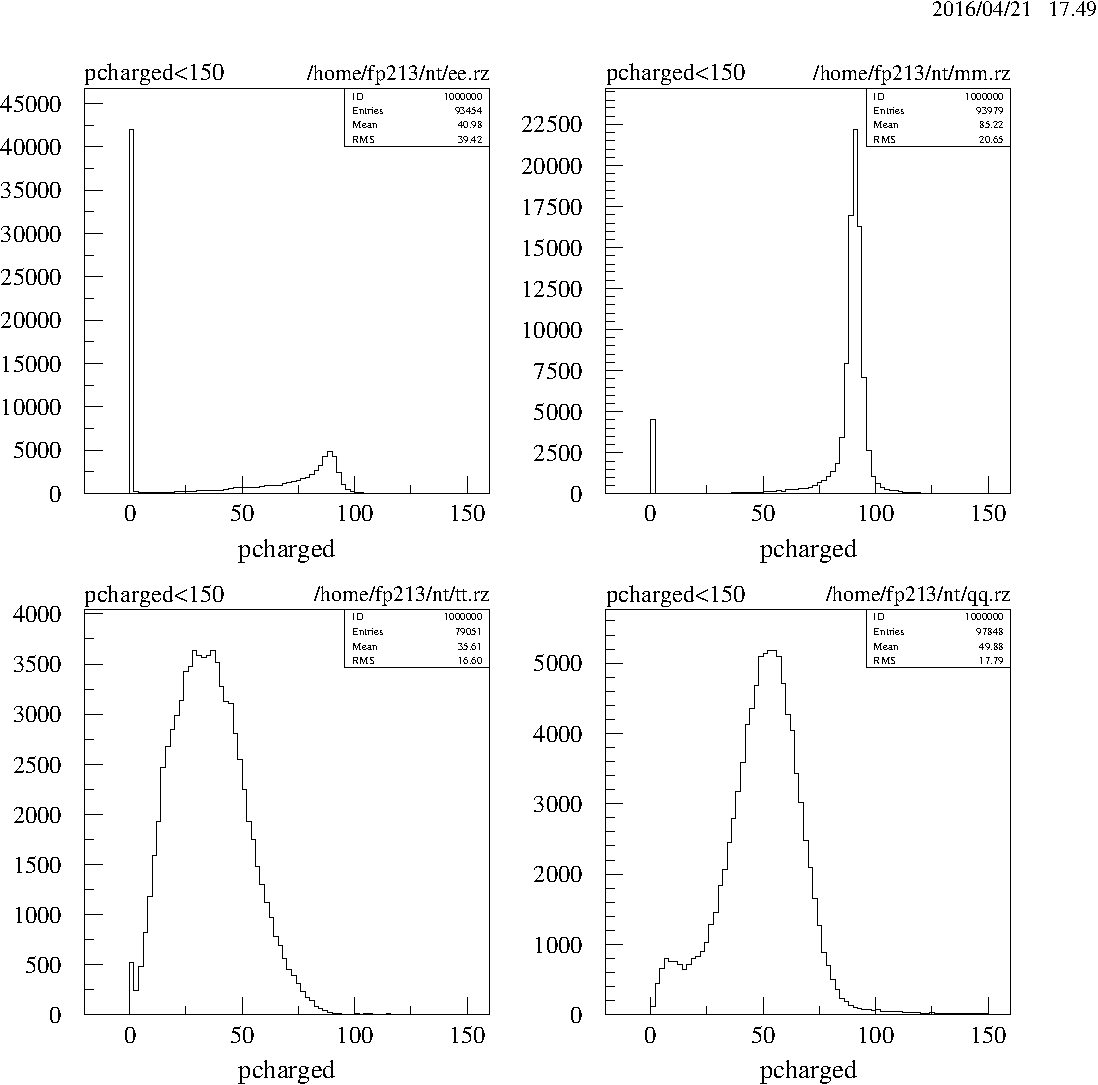
\includegraphics[width=1\textwidth]{./data/tag2/uncut/cropped/pcharged_uncut.pdf}
	\caption{text}
\end{figure}

\begin{figure}[h]
	\centering
	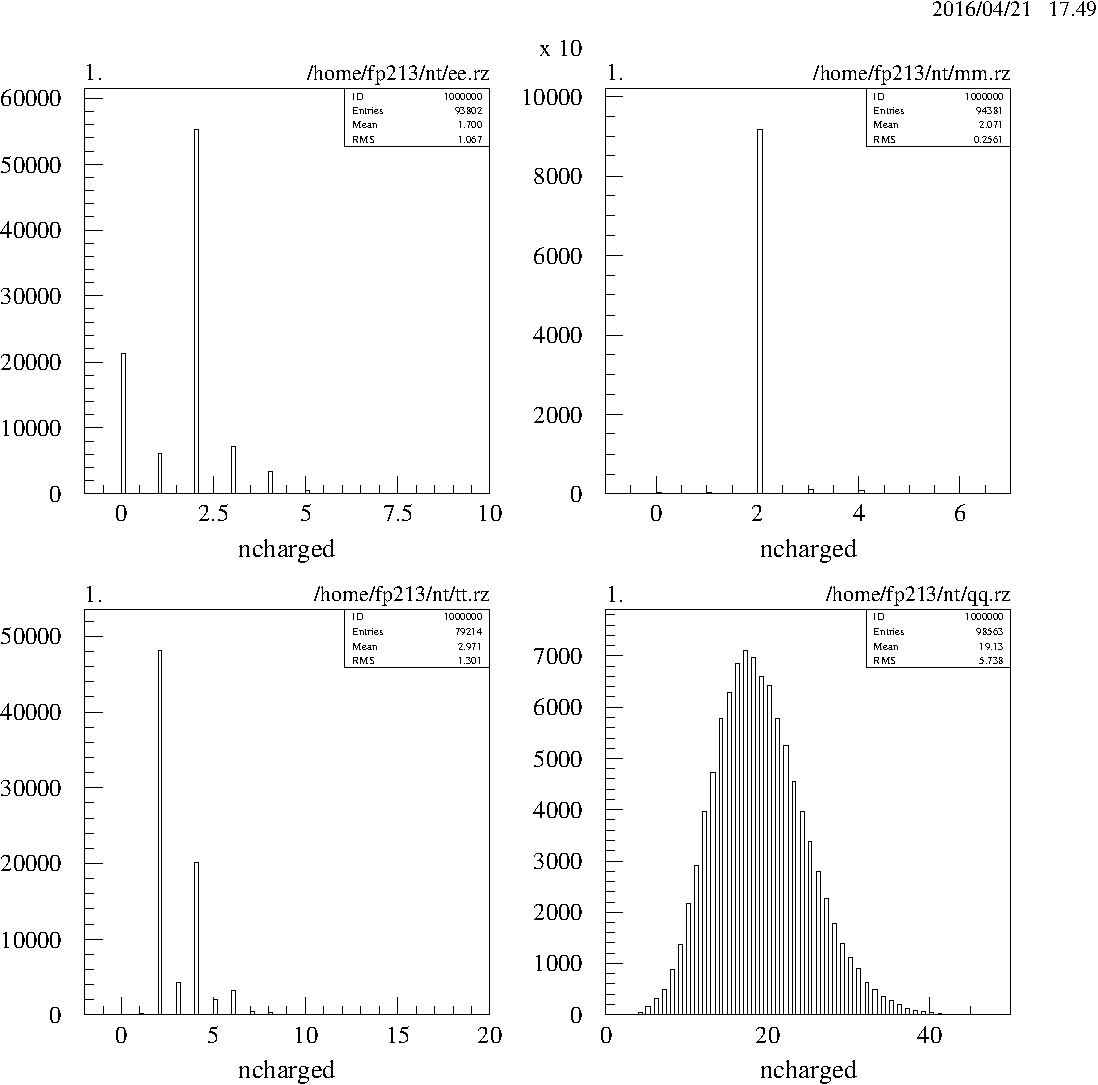
\includegraphics[width=1\textwidth]{./data/tag2/uncut/cropped/ncharged_uncut.pdf}
	\caption{text}
\end{figure}

\begin{figure}[h]
	\centering
	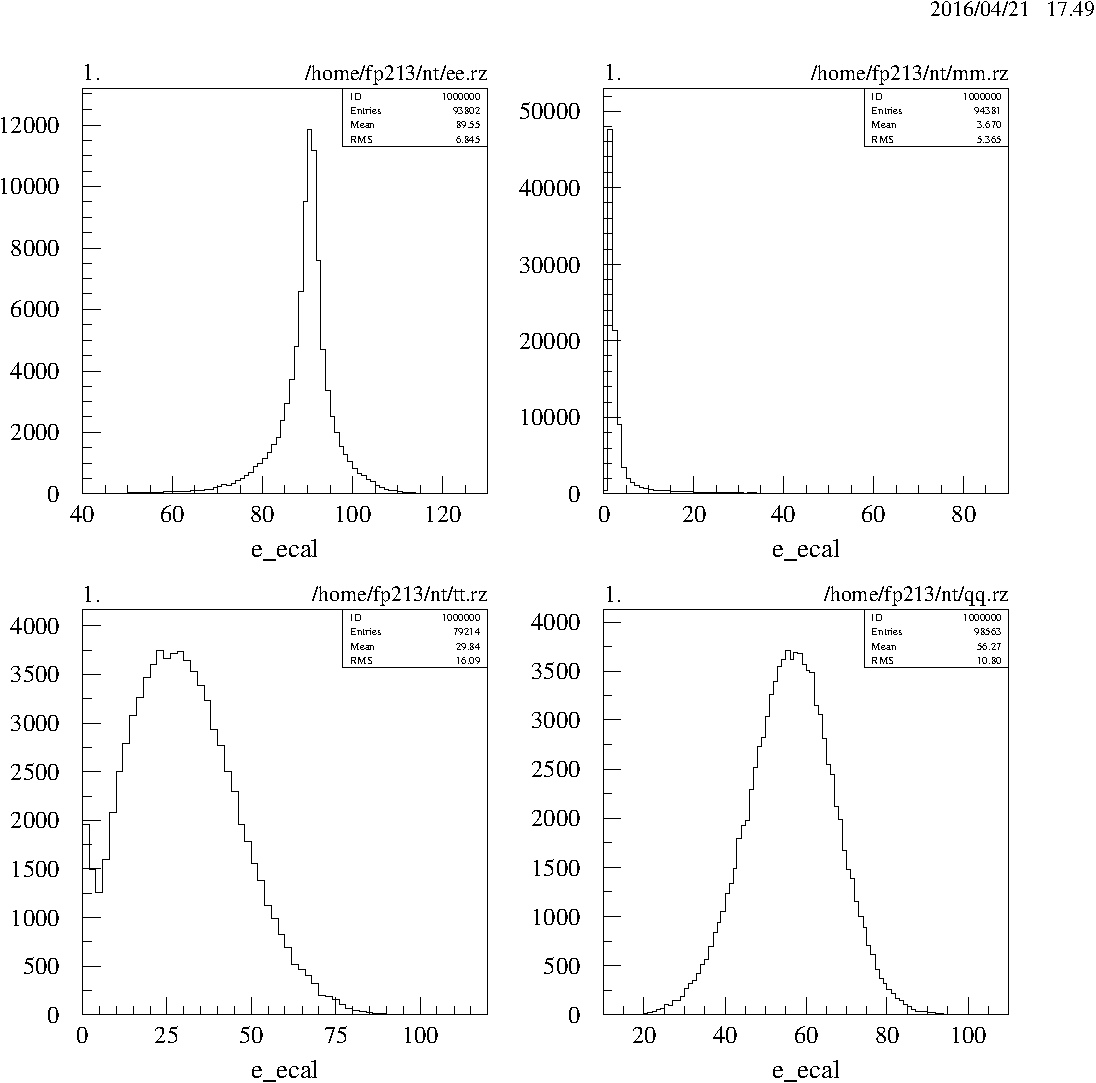
\includegraphics[width=1\textwidth]{./data/tag2/uncut/cropped/e_ecal_uncut.pdf}
	\caption{text}
\end{figure}

\begin{figure}[h]
	\centering
	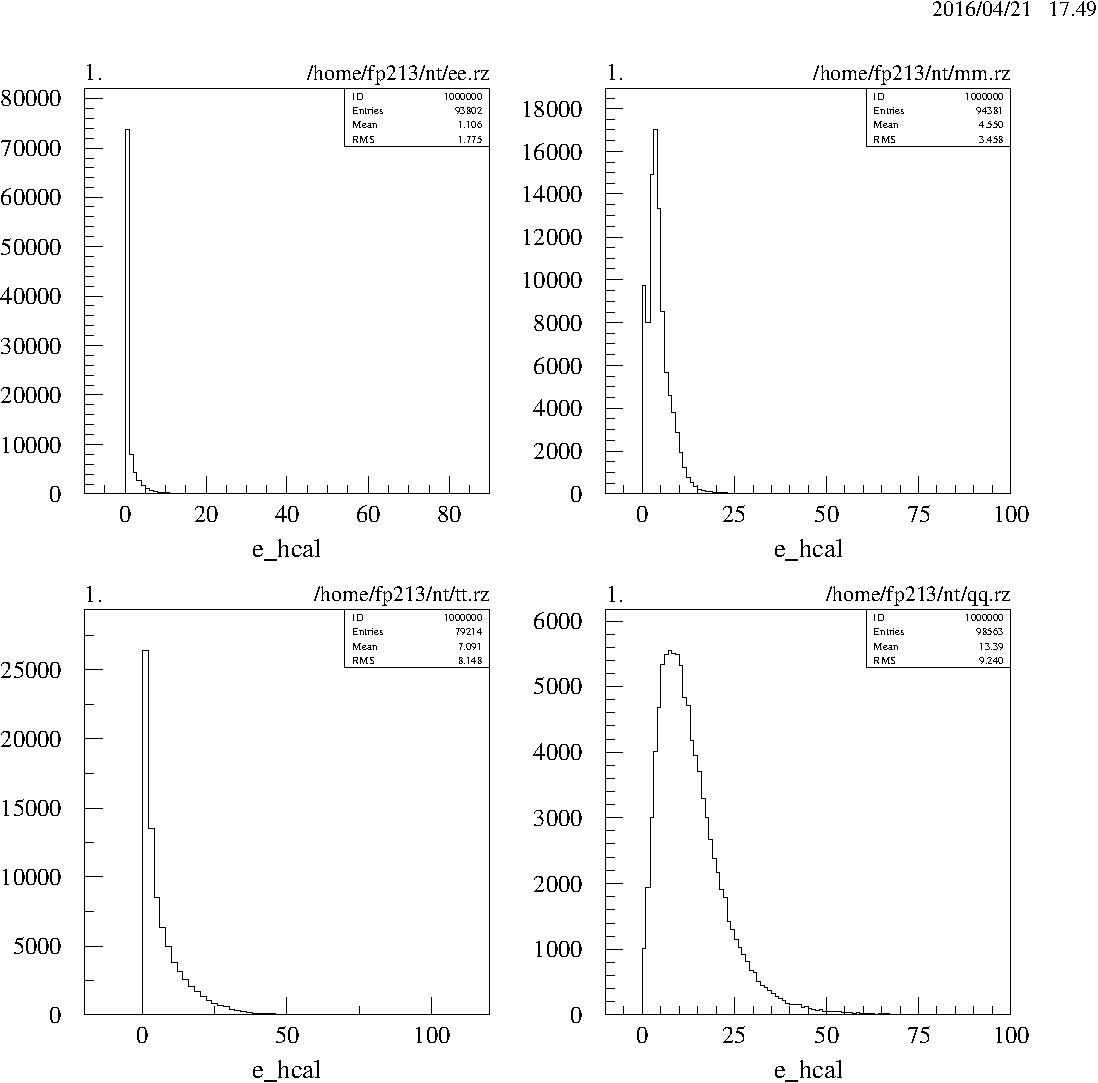
\includegraphics[width=1\textwidth]{./data/tag2/uncut/cropped/e_hcal_uncut.pdf}
	\caption{text}
\end{figure}

\begin{figure}[h]
	\centering
	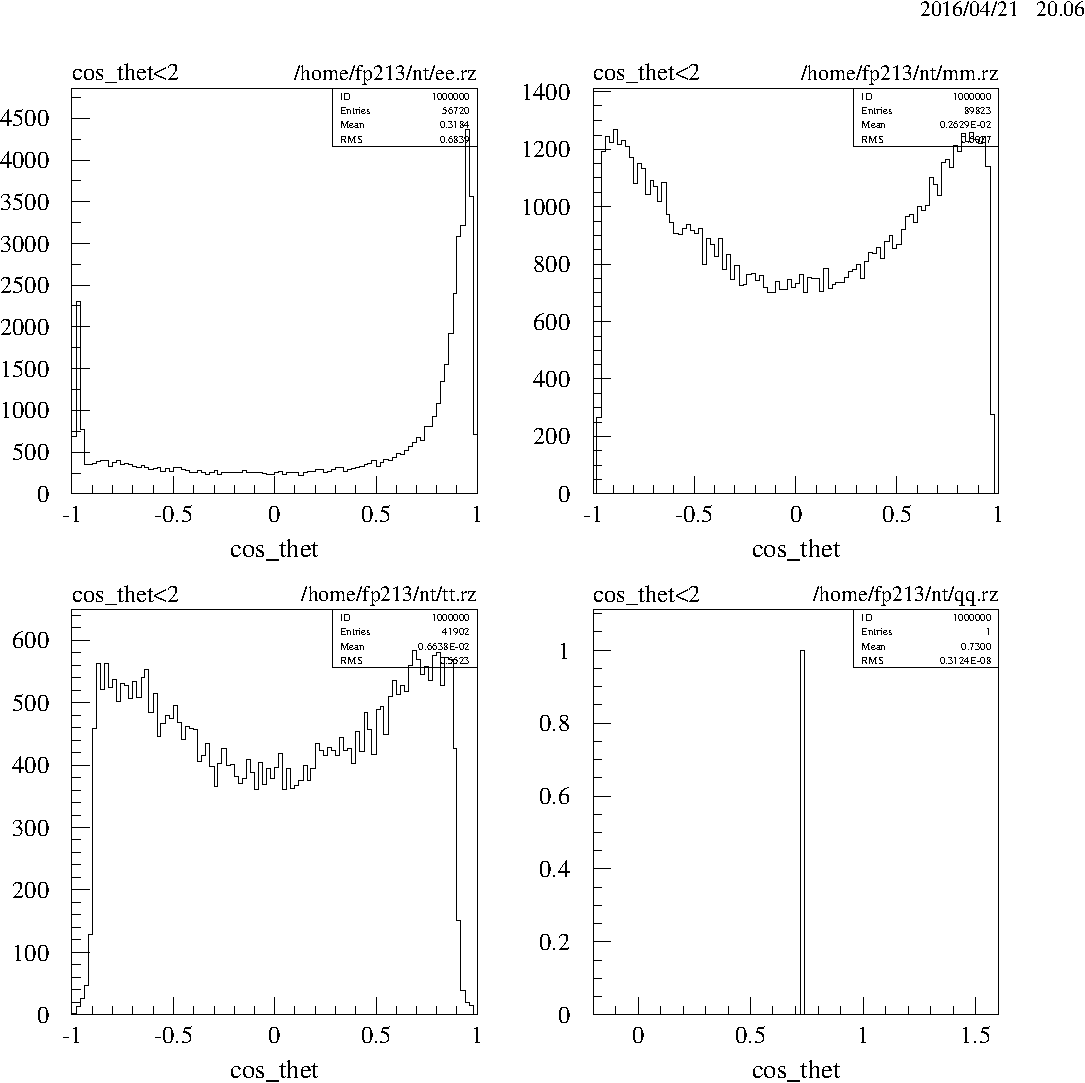
\includegraphics[width=1\textwidth]{./data/tag2/angular_mc/cropped/cos_theta.pdf}
	\caption{text}
	\label{fig:cos_theta_uncut}
\end{figure}


\clearpage
\subsection{MC-Data using the Final Cuts}
\label{app:mc_final_cut}

\begin{figure}
	\centering
	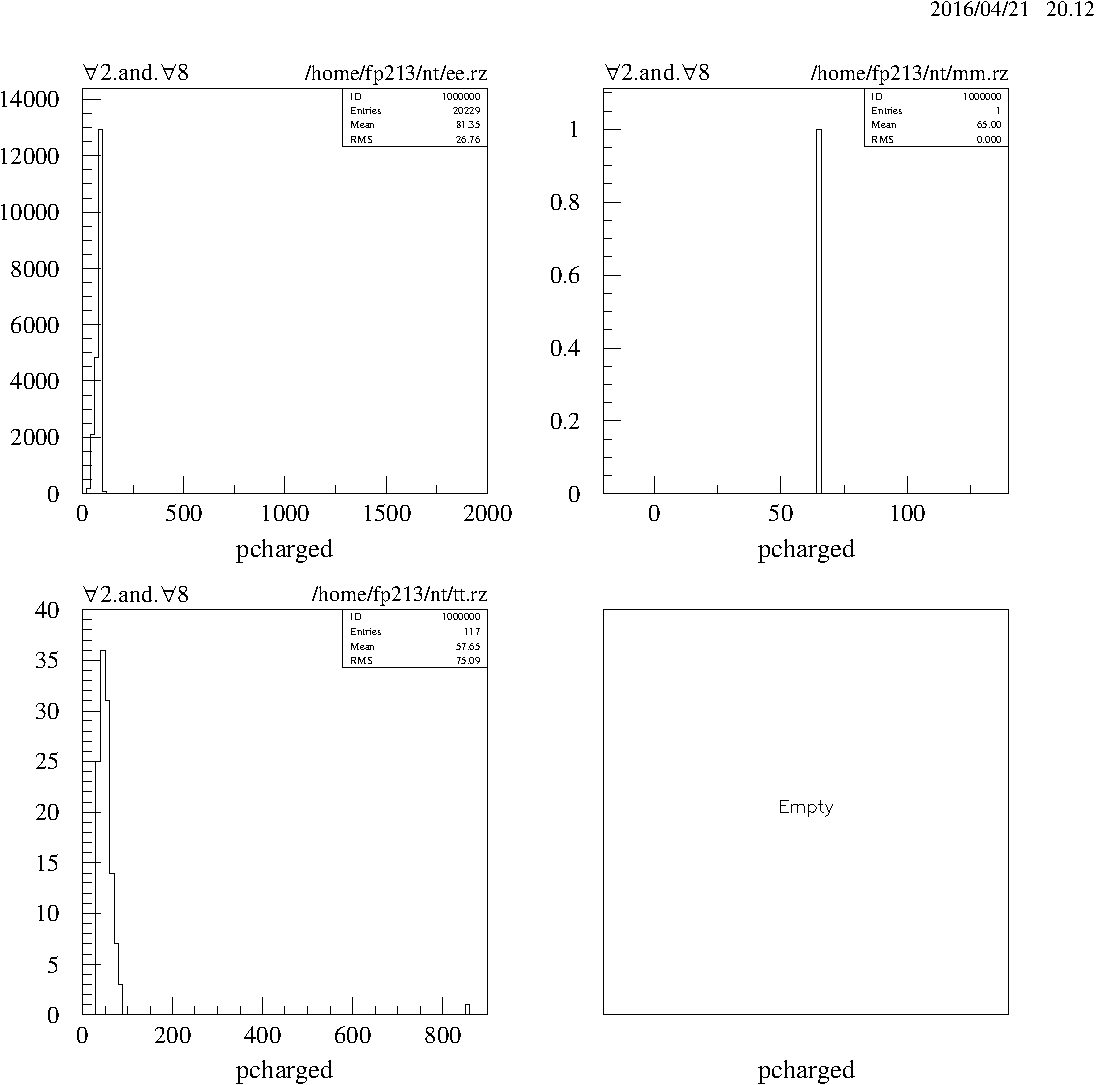
\includegraphics[width=1\textwidth]{./data/tag2/final_cuts/cropped/electron_cut.pdf}
	\caption{Electron cut}
\end{figure}

\begin{figure}
	\centering
	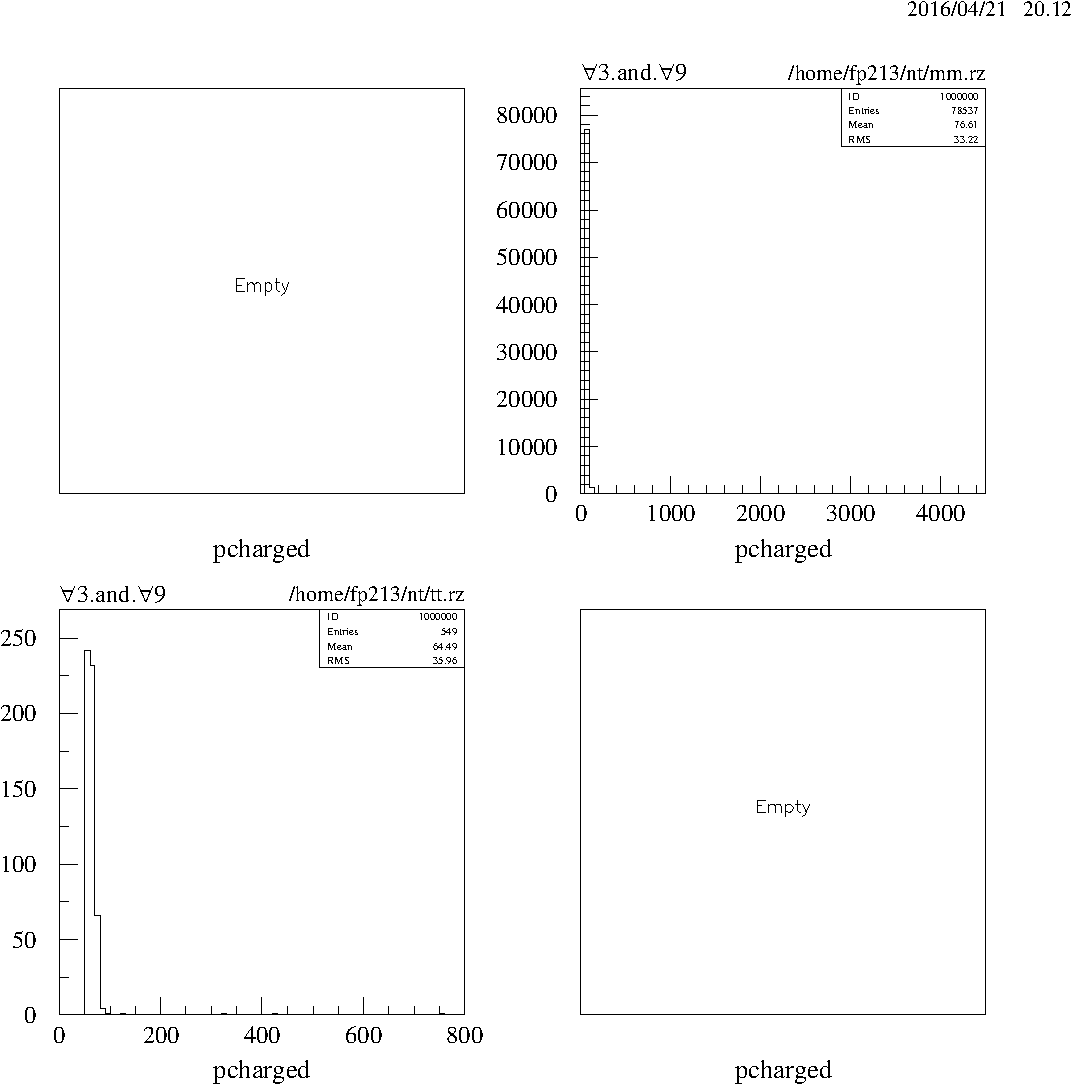
\includegraphics[width=1\textwidth]{./data/tag2/final_cuts/cropped/muon_cut.pdf}
	\caption{Muon cut}
\end{figure}

\begin{figure}
	\centering
	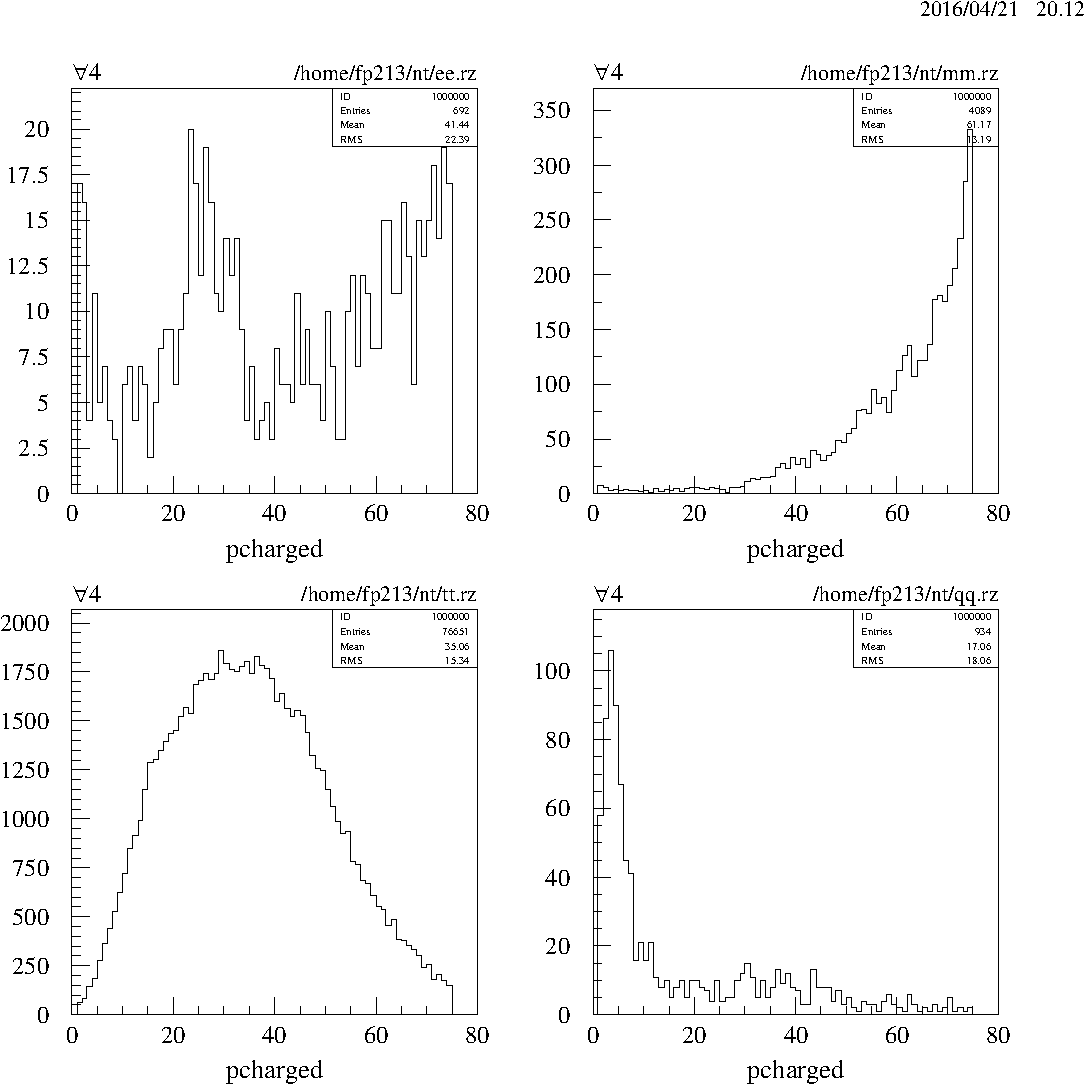
\includegraphics[width=1\textwidth]{./data/tag2/final_cuts/cropped/tau_cut.pdf}
	\caption{Tau cut}
\end{figure}

\begin{figure}
	\centering
	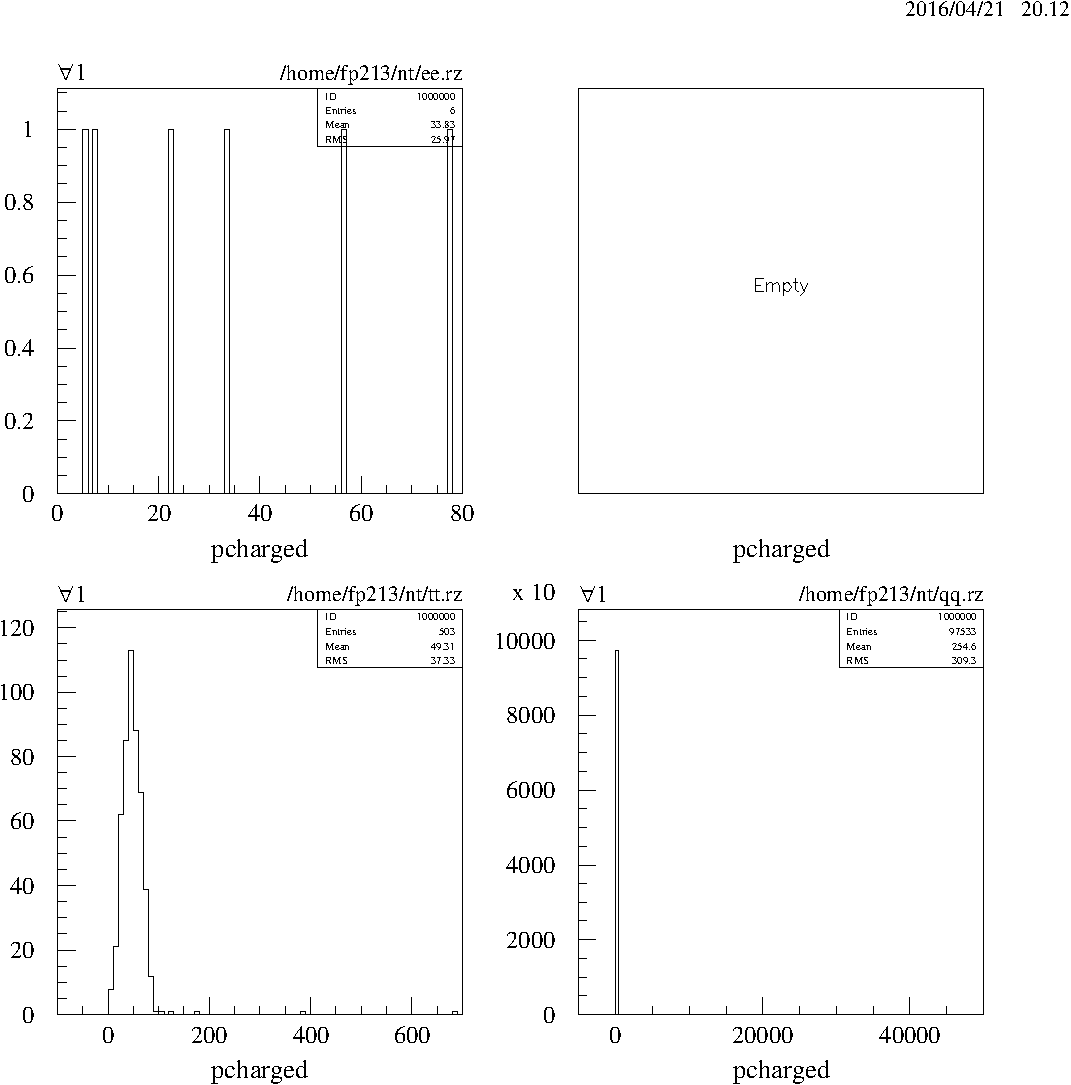
\includegraphics[width=1\textwidth]{./data/tag2/final_cuts/cropped/hadron_cut.pdf}
	\caption{Hadron cut}
\end{figure}






\end{appendix}

\end{document}
